%styles
%Da Latex für englischsprachige Texte ausgerichtet ist,
%wird als Dokumentenklasse das "`scrbook"' von Markus Kohm verwendet.
%Dieses ist für deutschsprachige Texte ausgelegt.
%BCOR12mm: 12mm Bindekorrektur (Verbreiterung des linken Randes)
%DIV11: entspricht in etwas der geforderten Textgröße und Seitenränder
%titlepage: eine Titelseite wird verwendet
%a4paper: DIN A4
%oneside: für eine spätere einseitige Bedruckung
\documentclass[BCOR12mm,DIV11,titlepage,a4paper,oneside,10pt]{scrbook}


% Farben definieren
\usepackage{color}
\usepackage[html]{xcolor}
\definecolor{m_green}{HTML}{00AD2F}
%\definecolor{m_pink}{HTML}{D40B6F}
\definecolor{m_pink}{HTML}{dd1166}
\definecolor{m_grey}{HTML}{555555}
\definecolor{m_lila}{HTML}{9313ce}
\definecolor{m_blau}{HTML}{4952e1}

% Paket Positionierung von Grafiken
\usepackage[export]{adjustbox}

%Paket für deutsche Silbentrennung etc.
\usepackage{ngerman}

%Paket für Zeichenkodierung, entspricht UTF-8
\usepackage[utf8x]{inputenc}

\usepackage{tocloft}
\newcommand{\listfootnotesname}{Fußnoten}% 'Fußnoten' title
\newlistof{footnotes}{fnt}{\listfootnotesname}% New 'List of...' for footnotes
\let\oldfootnote\footnote % Save the old \footnote{...} command
\renewcommand\footnote[1]{% Redefine the new footnote to also add 'List of Footnote' entries.
    \refstepcounter{footnotes}% Add and step a reference to the footnote/counter.
    \oldfootnote{#1}% Make a regular footnote.
    \addcontentsline{fnt}{footnotes}{\protect\numberline{\thefootnotes}#1}% Add the 'List of...' entry.
}

\newcommand{\listattachmentsname}{Anhang}% 'Anhang' title
\newlistof{attachments}{att}{\listattachmentsname}% New 'List of...' for attachments

%Paket das die Ausgabefonts definiert
\usepackage[T1]{fontenc}

%Paket für das Einbinden von Grafiken über die figure-Umgebung
\usepackage{graphicx}
\usepackage{grffile}

\usepackage{float}

\usepackage{mdframed}
\newmdenv[
  topline=false,
  bottomline=false,
  rightline=false,
  linewidth=2pt,
  linecolor=m_pink,
  innertopmargin=14pt,
  innerbottommargin=14pt,
  backgroundcolor=black!5,
  skipabove=\topsep,
  skipbelow=\topsep
]{siderules}

%Paket für mehrseitige Tabellen
\usepackage{longtable}
\setlength\LTleft{0pt}
\setlength\LTright{0pt}

\usepackage{booktabs}

%Paket zum \UTF{0192}ndern der Kopf- und Fußzeile
\usepackage{fancyhdr}

%Benutzt das Paket für eigenen Seitenstil
\pagestyle{fancy}

%Erzeugt eine Linie in der Kopfzeile (lässt sich mit 0.0pt ausblenden)
\renewcommand*{\headrulewidth}{0.1pt}
\renewcommand{\headrule}{\hbox to\headwidth{%
  \color{m_pink}\leaders\hrule height \headrulewidth\hfill}}
\lhead{} %Kopfzeile links

%\chead{\thepage} %Kopfzeile mitte
\chead{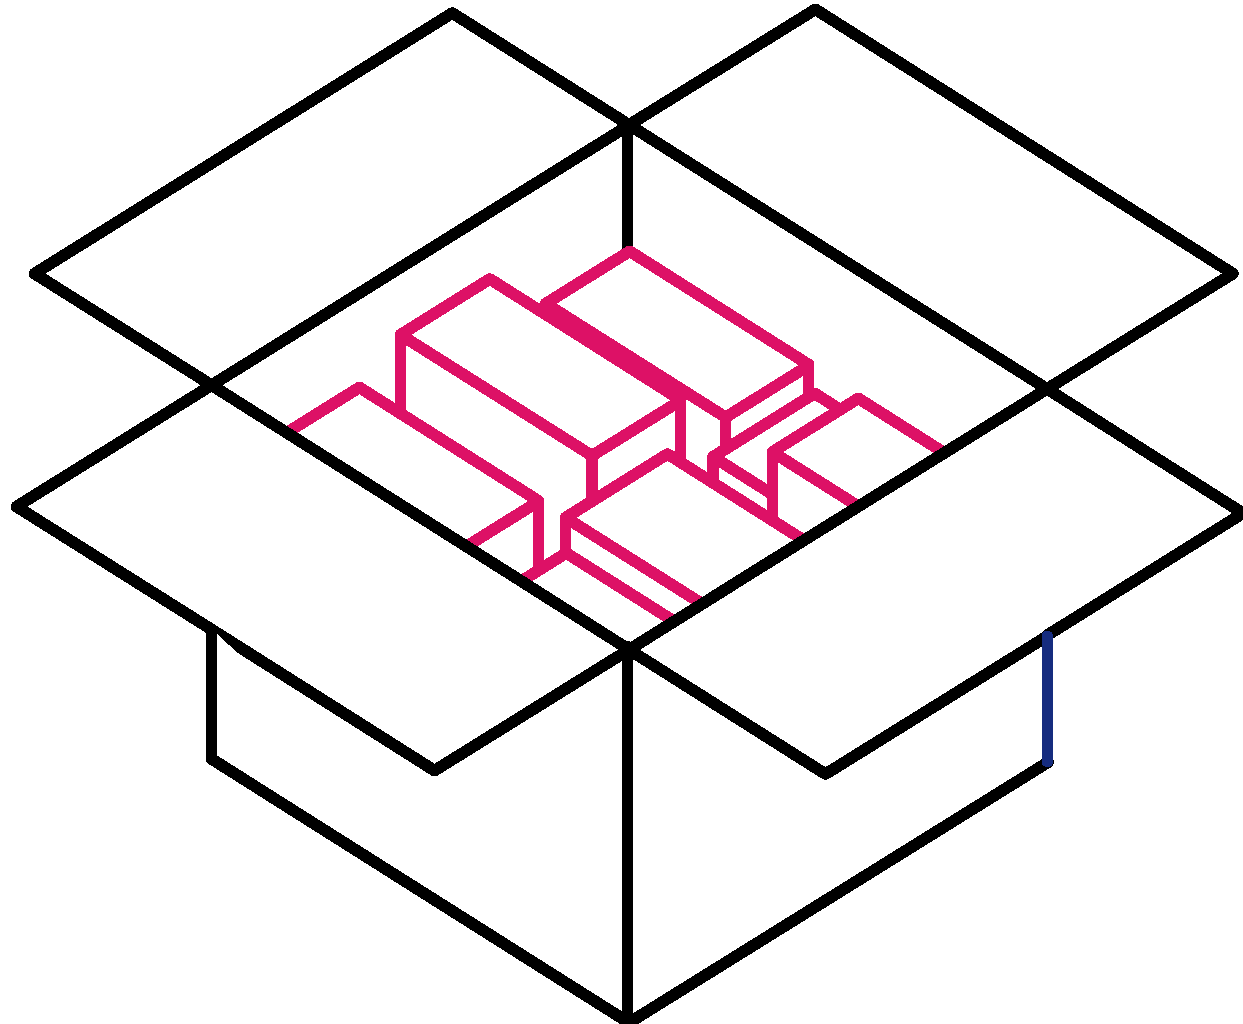
\includegraphics[height=20pt]{../assets/box.pdf}}
\rhead{} %Kopfzeile rechts
\lfoot{} %Fußzeile links
\cfoot{} %Fußzeile mitte
\rfoot{} %Fußzeile rechts
\makeatother


\newcommand{\changefont}{%
    \fontsize{9}{11}\selectfont
}


\setlength\headheight{60pt}
\setlength\footheight{40pt}
%\lfoot{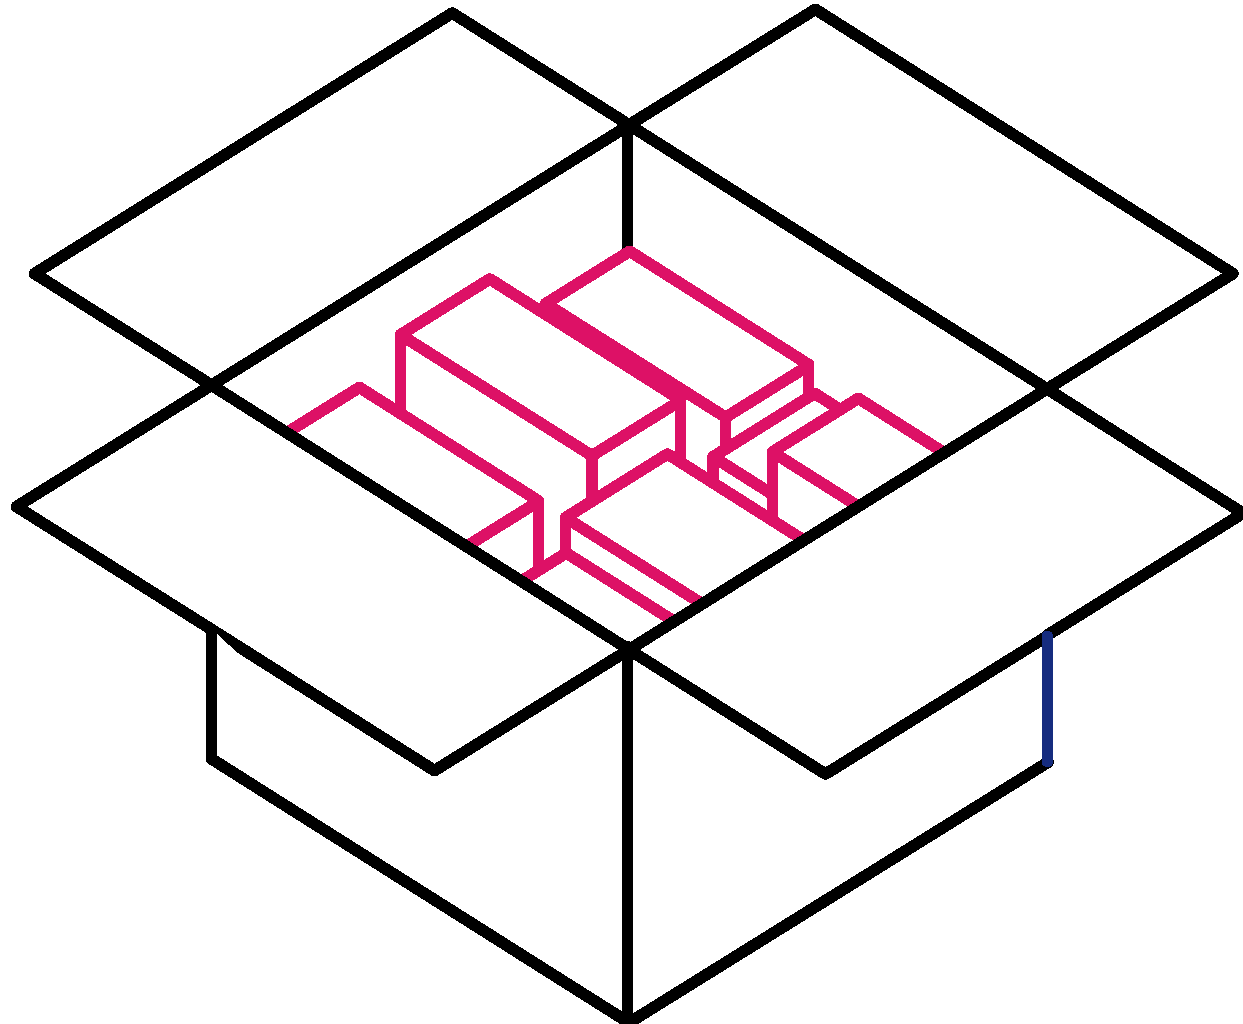
\includegraphics[height=40pt]{../assets/box.pdf}}
\rfoot{\thepage}
\lfoot{\changefont <| title |> Medieninformatik\\TH Köln // Institut für Informatik\\ \today}


%\UTF{0192}ndert die Seitennummerierung beim Inhaltsverzeichnis mit eigenem Stil
\renewcommand*{\indexpagestyle}{fancy}
%Verhindert die Seitennummerierung auf den Part-Seiten
\renewcommand*{\partpagestyle}{empty}
%\UTF{0192}ndert die Seitennummerierung bei Chapter mit eigenem Stil
\renewcommand*{\chapterpagestyle}{fancy}

%Abbildungsnummerierung ändern (abhängig von chapter, z.B. Abbildung 1.1)
\renewcommand*{\thefigure}{\thechapter.\arabic{figure}}
%Tabellennummerierung ändern (abhängig von chapter, z.B. Tabelle 1.1)
\renewcommand*{\thetable}{\thechapter.\arabic{table}}

%Paket, um ein Glossar/Abkürzungsverzeichnis anzulegen
\usepackage{nomencl}
\let\abbrev\nomenclature
%Der Name wird in Glossar geändert
\renewcommand{\nomname}{Glossar}
%Definiert die Aufteilung im Glossar zwischen Begriffen und Erläuterung
\setlength{\nomlabelwidth}{.25\hsize}
%Definiert die Punktelinien im Glossar
\renewcommand{\nomlabel}[1]{#1 \dotfill}
\setlength{\nomitemsep}{-\parsep}
%Veranlasst die Erstellung des Glossars
\makenomenclature

%Einrückungen nach Absätzen und Grafiken verhindern
\setlength{\parindent}{0pt}

%Verhindern, dass eine neue Seite für ein einzelnes Wort/Zeile verwendet wird
\clubpenalty = 10000 % schliesst Schusterjungen aus
\widowpenalty = 10000 % schliesst Hurenkinder aus (keine Beleidigung, sondern wirklich ein Fachbegriff)

%Paket für ein deutsches Literaturverzeichnis
\usepackage{bibgerm}

%Paket für die Verwendung von URLs durch den Befehl \url{}
%\usepackage{url}
\usepackage[hyphens]{url}

%Paket für Zeilenabstand (onehalfspace, singlespace)
\usepackage{setspace}

%Paket zur Erzeugung von Anführungszeichen durch \enquote{Text}
% \usepackage[ngerman]{babel}
% \usepackage[babel, german=quotes]{csquotes}

%Paket für farbigen Text
%black,white,green,red,blue,yellow,cyan,magenta
\usepackage{color}

%Paket für farbigen Hintergrund für Verbatim-Umgebung (Quelltext-Umgebung)
\usepackage{fancyvrb}
\usepackage{verbatim,moreverb}
%Grauton für Quelltext-Umgebung definieren 80% Grau
\definecolor{sourcegray}{gray}{.80}
%Paket für Quelltext-Umgebung
\usepackage{listings}

%Paket für Positionierung der Objekte ohne Float (Verwendungsbsp.: \begin{figure}[H])
\usepackage{float}

%Paket zur Erzeugung von Hyperrefs und PDF Informationen
\usepackage[pdftex,plainpages=false,pdfpagelabels,
            pdftitle={ <| title |> Medieninformatik // TH Köln // Institut für Informatik},
            pdfauthor={}
            ]{hyperref}
\hypersetup{
    colorlinks = true
}
\usepackage{pdfpages}

\providecommand{\tightlist}{%
  \setlength{\itemsep}{0pt}\setlength{\parskip}{0pt}}

\usepackage{tabularx}
\newcolumntype{L}[1]{>{\raggedright\arraybackslash}p{#1}}
\newcolumntype{C}[1]{>{\centering\arraybackslash}p{#1}}
\newcolumntype{R}[1]{>{\raggedleft\arraybackslash}p{#1}}

% URL
\PassOptionsToPackage{hyphens}{url}
\usepackage[pdftex]{hyperref}

% Sonderzeichen
\usepackage{textcomp}
\usepackage{eurosym}

\usepackage{setspace}
\renewcommand{\baselinestretch}{1.2}
\setlength{\parskip}{1em}

\usepackage[sfdefault,light]{roboto}  %% Option 'sfdefault' only if the base font of the document is to be sans serif


\usepackage[raggedright]{titlesec}
\titleformat{\chapter}[display]
  {\normalfont\sffamily\mdseries}
  {}{14pt}{\huge\raggedright}
% {\chaptertitlename\ \thechapter}{14pt}{\huge\raggedright}
\titleformat{\section}
  {\singlespacing\normalfont\sffamily\mdseries\Large\color{m_pink}\raggedright}
  {\thesection}{1em}{\Large}
\titleformat{\subsection}
  {\singlespacing\normalfont\sffamily\mdseries\large\raggedright}
  {\thesubsection}{1em}{\large}
% Zeilenumbruch und Spacing für Absätze
\titleformat{\paragraph}[hang]
  {\singlespacing\normalfont\normalsize\bfseries}
  {\theparagraph}{1em}{}
\titlespacing*{\paragraph}{0pt}{3.25ex plus 1ex minus .2ex}{0.5em}


\usepackage[font=footnotesize]{caption}


% Footer definieren
\makeatletter
\def\footrule{{
  \vskip-\footruleskip\vskip-\footrulewidth
  \color{\footrulecolor}
  \hrule\@width\headwidth\@height
  \footrulewidth\vskip\footruleskip
}}
\makeatother
\renewcommand{\footrulewidth}{0.1pt}
\newcommand{\footrulecolor}{m_green}



\begin{document}

%=== Deckblatt =======================================================
% Coversheet

\begin{titlepage}

	
\includegraphics[width=0.25\textwidth]{../../../assets/logo_th_koeln.pdf}

	\vspace{2cm}
	{\Large\raggedright Stellungnahme zum Akkreditierungsbericht der Gutachter\par}
	\vspace{1cm}
	{\Large TH Köln – Campus Gummersbach \\ Fakultät für Informatik und Ingenieurwissenschaften \\ Institut für Informatik\par}

	\vfill

% Bottom of the page
	{\large \today\par}
\end{titlepage}


%=== Inhaltsverzeichnis ==============================================
\tableofcontents

%=== Hauptteil =======================================================
%Seitennummerierung des Hauptteils
\mainmatter


\chapter{Einführung\label{/mi-2017/modulbeschreibungen-master/schwerpunkte-einfuehrung}}\label{einfuxfchrungpathlabelmi-2017modulbeschreibungen-masterschwerpunkte-einfuehrung}

Im Masterstudium Medieninformatik können AbsolventInnen von
Studiengängen der Informatik ihre Kompetenzen vertiefen und erweitern.
Dabei geht es um die Gestaltung, Produktion, Bearbeitung, Distribution
und Nutzung medienbasierter Informationen. Im Masterstudium lernt man,
wie sich web-basierte Prozesse und Systeme analysieren, entwerfen,
realisieren, adaptieren, betreiben und evaluieren lassen.

Der Masterstudiengang Medieninformatik ist durch seine
Studienschwerpunkte Human Computer Interaction, Multi-Perspective
Product Development, Social Computing, Visual Computing und Weaving the
Web charakterisiert.

Im Zentrum des Studiums steht in den ersten drei Fachsemestern jeweils
eine Projektarbeit, in der die Anwendung von Fachwissen,
wissenschaftliche Methoden, der fachliche Diskurs, die selbstständige
Urteilsfindung und das fachpraktische Handeln in komplexen
Projektkontexten und interdisziplinären Teams eingeübt werden. Die drei
Projekte sind den Projektphasen Konzeption, Entwicklung und Verwertung
zugeordnet, sodass sowohl die Studierenden als auch die Projekte alle
Phasen durchlaufen. Ein wesentlicher Leitgedanke dieser Projektphasen
ist, dass Projektergebnisse - basierend auf der Phase Verwertung - den
Weg in die Öffentlichkeit finden sollten: als Veröffentlichung, als
social-coding-Projekt oder sogar als Start Up.

Das erforderliche Grundlagenwissen sowie schwerpunktbezogene Kenntnisse
werden in den ersten drei Semestern parallel zur Projektarbeit in drei
Grundlagen-, drei Schwerpunkt- und drei Wahlpflicht-Modulen sowie in
projektbegleitenden Lehrveranstaltungen vermittelt. Das vierte Semester
ist dann darauf aufbauend ganz der selbstständigen Arbeit an der
Masterthesis gewidmet.

\begin{figure}[htbp]
\centering
\includegraphics[width=\columnwidth]{../anhaenge/bilder/ws-small.png}
\caption{Studienverlaufsplan Medieninformatik Master, Studienbeginn zum
Wintersemester}
\end{figure}

\begin{figure}[htbp]
\centering
\includegraphics[width=\columnwidth]{../anhaenge/bilder/ss-small.png}
\caption{Studienverlaufsplan Medieninformatik Master, Studienbeginn zum
Sommersemester}
\end{figure}

\chapter{Schwerpunkt: Human-Computer
Interaction\label{/mi-2017/modulbeschreibungen-master/schwerpunkt-human-computer-interaction}}\label{schwerpunkt-human-computer-interactionpathlabelmi-2017modulbeschreibungen-masterschwerpunkt-human-computer-interaction}

\section*{Allgemeines\label{/mi-2017/modulbeschreibungen-master/schwerpunkt-human-computer-interaction}}\label{allgemeinespathlabelmi-2017modulbeschreibungen-masterschwerpunkt-human-computer-interaction}

Medieninformatik und Mensch-Computer Interaktion stehen in vielerlei
Hinsicht in einem engen Zusammenhang. So beinhaltet etwa der Fachbereich
„Mensch-Computer Interaktion`` der GI e.V. die
\href{http://fb-mci.gi.de/mensch-computer-interaktion-mci/fachgruppen/medieninformatik.html}{Fachgruppe
„Medieninformatik``}.

Im Zusammenhang mit der „third wave of HCI`` (Susan Bødker, 2006 und
2016) wird die aktuelle Bedeutung der Disziplin der Mensch-Computer
Interaktion für die Gestaltung interaktiver Systeme und insbesondere
ihre Rolle für die Medieninformatik deutlich. Nach Bødker besteht eine
aktuelle Herausforderung der 3rd wave of HCI insbesondere darin, dass
sich die Trennlinie von Technologienutzung zwischen
beruflichem/gewerblichem und privatem Bereich mehr und mehr auflöst.
Medieninformatik befasst sich insbesondere mit interaktiven und
multimedialen Systemen in gewerblichen und privaten Nutzungskontexten
und adressiert demnach die Herausforderungen der 3rd wave of HCI.

\section*{Zielsetzungen\label{/mi-2017/modulbeschreibungen-master/schwerpunkt-human-computer-interaction}}\label{zielsetzungenpathlabelmi-2017modulbeschreibungen-masterschwerpunkt-human-computer-interaction}

Dieser Schwerpunkt adressiert Kompetenzen, Fähigkeiten und Fertigkeiten
die im Zusammenhang mit der Leitung und dem Management von
Entwicklungsprojekten innovativer, interaktiver Systeme stehen. Dies
umfasst die Nutzungskontexte in verschiedensten Anwendungsbereichen
kritisch zu analysieren, Problemfelder zu identifizieren, Anforderungen
zu spezifizieren, angemessene Vorgehen zur Lösungsentwicklung zu
konzipieren und Gestaltungslösungen zu entwickeln und zu evaluieren.
Absolventen dieses Schwerpunktes arbeiten als UX-Architects, Interaction
Designer oder in Positionen mit ähnlichen Rollenbezeichnungen in
Unternehmen/Institutionen und sind zentrale Entscheidungsträger, wenn es
um die Entwicklung interaktiver Systeme aus Nutzungs -oder
Nutzerperspektive geht.

Neben den vielfältigen weiterentwickelten Kompetenzen (formale,
analytische, methodologische, gestalterische, technologische, etc.)
haben sie die Befähigung zum fachlichen Diskurs vertieft und
implementieren mit ihrer Kommunikationskompetenz eine wichtige
Schnittstelle für die verschiedenen Stakeholder und Gewerke.

\section*{Berufsbilder\label{/mi-2017/modulbeschreibungen-master/schwerpunkt-human-computer-interaction}}\label{berufsbilderpathlabelmi-2017modulbeschreibungen-masterschwerpunkt-human-computer-interaction}

Hier werden exemplarisch lediglich zwei Berufsbilder genannt. Weitere
Berufsbilder sind User Experience Designer, User Experience Architect
u.v.m.; allerdings variieren die Bezeichnungen, je nach dem, welches
Unternehmen, welche Institution etc. man betrachtet. In sofern erhebt
die hier vorliegende Nennung und Darstellung nicht den Anspruch auf
Vollständigkeit sondern versucht lediglich, einige wenige etablierte
Berufsbilder zu umreissen.

\textbf{Usability Engineer}

Usability Engineers arbeiten entweder direkt im Unternehmen oder in der
Beratung von Unternehmen. Ihre maßgebliche Aufgabe ist es, über den
gesamten Lebenszyklus für eine hohe Gebrauchstauglichkeit interaktiver
sozio-technischer System zu sorgen. Dazu wenden Sie Prinzipien,
Vorgehensweisen, Methoden und Arbeitstechniken der Disziplin
„Mensch-Computer Interaktion`` an. Sie planen Entwicklungsprozesse,
analysieren Lebens- und Nutzungskontexte von Nutzergruppen, analysieren
und spezifizieren Nutzungsanforderungen, entwerfen Gestaltungslösungen
und analysieren/evaluieren diese. Darüber hinaus kommunizieren Sie mit
allen Berufsgruppen, die bei der Konzeption, Gestaltung, Entwicklung,
Evaluation und dem Betrieb dieser interaktiven Systeme beteiligt sind
und übernehmen damit quasi die Rolle eines Anwalts der Benutzer.

\textbf{Interaction Designer}

Interaction Designer konzipieren und gestalten die vielfältigen
Beziehungen zwischen Menschen und Technologien. Diese Beziehungen sind
unter anderem ökonomischer, sozialer, ökologischer, kulturell/ethischer
aber auch ästhetischer Art. Anders als bei der eher
ingenieurswissenschaftlichen Herangehensweise der Usability Engineers
denken und handeln Interaction Designer wie Designer. Dies bedeutet,
dass Interaction Designer in ähnlichen Projekten tätig sind, aber mit
einer ausgeprägten kreativen Problemlösungskompetenz auf methodischer
Ebene sowie einer reflektierten und eigenverantwortlichen
Entscheidungskompetenz ausgestattet sind. Sie können sicherstellen, dass
sich Technologie nach gewünschten Wertmaßstäben nahtlos und positiv in
den Lebensalltag von Menschen eingliedert. Damit geht Interaction Design
weit über die reine Konzeption und Gestaltung von Eingaben und Ausgabe
an der Benutzungsschnittstelle (User Interface Designer).

\section*{Schwerpunktspezifische
Pflichtmodule\label{/mi-2017/modulbeschreibungen-master/schwerpunkt-human-computer-interaction}}\label{schwerpunktspezifische-pflichtmodulepathlabelmi-2017modulbeschreibungen-masterschwerpunkt-human-computer-interaction}

\begin{itemize}
\tightlist
\item
  \hyperref[/mi-2017/modulbeschreibungen-master/MA_HCI_InteractionDesign]{Interaction
  Design}
\item
  \hyperref[/mi-2017/modulbeschreibungen-master/MA_HCI_Design_Methodologies]{Design
  Methodologies}
\item
  \hyperref[/mi-2017/modulbeschreibungen-master/MA_HCI_Modul_Statistical_Methods_for_HCI]{Angewandte
  Statistik für die Mensch-Computer Interaktion}
\end{itemize}

\chapter{Schwerpunkt: Multiperspective Product
Development\label{/mi-2017/modulbeschreibungen-master/schwerpunkt-multiperspective-product-development}}\label{schwerpunkt-multiperspective-product-developmentpathlabelmi-2017modulbeschreibungen-masterschwerpunkt-multiperspective-product-development}

\section*{Allgemeines\label{/mi-2017/modulbeschreibungen-master/schwerpunkt-multiperspective-product-development}}\label{allgemeinespathlabelmi-2017modulbeschreibungen-masterschwerpunkt-multiperspective-product-development}

Im Schwerpunkt ``Multi-Perspective Product Development'' entwickeln und
vertiefen die Studierenden ihre Kompetenz, die typische Heterogenität
vieler Medieninformatik-Projekte von der Methodik über die
technologische bis hin zur sozio-technischen Komponente zu verstehen und
zu bewältigen. In solchen Projekten haben die unterschiedlichen
Stakeholder oft eigene Perspektiven, die durch ihre Fachsprachen,
Methoden und Techniken sowie Verantwortlichkeiten definiert werden. Die
Schnittstellen zwischen diesen Perspektiven sind in aller Regel nicht
offensichtlich, da das Wissen oft implizit ist oder in vielfältiger
Weise dargestellt wird. Die Studieninhalte sind daher entsprechend
dieser heterogenen Bedingungen eher breit angelegt. Das Studienziel ist
die Qualifikation, in Projekten der Medieninformatik auf breiter
wissenschaftlicher Basis federführend mitzuwirken und sie organisieren
und leiten zu können.

\section*{Zielsetzungen\label{/mi-2017/modulbeschreibungen-master/schwerpunkt-multiperspective-product-development}}\label{zielsetzungenpathlabelmi-2017modulbeschreibungen-masterschwerpunkt-multiperspective-product-development}

Der Schwerpunkt „Multi-Perspective Product Development'' bereitet die
Studierenden auf die, für viele Projekte der Medieninformatik, typische
Heterogenität vor, welche von der methodologischen über die
technologische bis hin zur soziotechnischen Komponente reicht.
Chakterisierende Merkmale solcher Projekte sind:

\begin{itemize}
\tightlist
\item
  Berücksichtigung von und Kommunikation mit Stakeholdern mit jeweils
  eigenen Perspektiven, die durch ihre Fachsprache, Methoden und
  Techniken sowie entsprechende Fähigkeiten, Verantwortlichkeiten und
  Kompetenzen definiert werden.
\item
  Heterogene soziale, technologische und ökonomische Rahmenbedingungen
  wie z.B.
\item
  die Anwendung von unterschiedlichen, agilen bis hin zu
  „schwergewichtigen'' Vorgehensmodellen,
\item
  lokale Zusammenarbeit in kleinen Teams bis hin zu dezentraler
  Zusammenarbeit in großen, international und interdisziplinär
  aufgestellten Teams,
\item
  ein breites Spektrum der Projektgegenstände von kleinen, nativen Apps
  für mobile Geräte bis hin zu großen, geschäftskritischen,
  internationalisierbaren und responsiven Web-Anwendungen,
\item
  ein breites Spektrum der Projektkontexte von kleinen Inhouse-Projekten
  bis hin zu großen, organisationsübergreifenden internationalen
  Projekten.
\end{itemize}

\section*{Berufsbilder\label{/mi-2017/modulbeschreibungen-master/schwerpunkt-multiperspective-product-development}}\label{berufsbilderpathlabelmi-2017modulbeschreibungen-masterschwerpunkt-multiperspective-product-development}

Die multiperspektivische Anlage des Studienschwerpunkts berücksichtigt
das große berufliche Spektrum im Umfeld der Gestaltung, Entwicklung und
Evaluierung von Produkten, Diensten und Prozessen für Medien- und
Web-Anwendungen bis hin zu mobilen Apps. Daher wird hier kein
spezifisches Berufsbild angegeben, sondern eher eine grobe
Charakterisierung. Typische Branchen sind z.B.

\begin{itemize}
\tightlist
\item
  IT-Berater, Software- und Service-Dienstleister und -Betreiber
\item
  Print- und Online-Verlage
\item
  Game-Entwicklung
\item
  Marketing-, Werbe- und PR-Agenturen,
\item
  Filmproduktionsfirmen, Radio- und Fernsehanstalten sowie
\item
  Forschung und Entwicklung
\end{itemize}

Aufgrund der inhaltlich eher breiten Anlage können die
Absolvent\emph{inn}en des Studienschwerpunkts ``Multi-Perspective
Product Development'' in solchen Branchen sowohl als
Softwareentwickler\emph{In} für IT-Lösungen in den oben genannten
Branchen tätig sein, aber auch als Anforderungsermittler\emph{In},
Gestalter\emph{In} von Benutzeroberflächen von IT-Anwendungen sowie in
Projektmanagement, Qualitätssicherung und Qualitätsmanagement wirken.

\section*{Schwerpunktspezifische
Pflichtmodule\label{/mi-2017/modulbeschreibungen-master/schwerpunkt-multiperspective-product-development}}\label{schwerpunktspezifische-pflichtmodulepathlabelmi-2017modulbeschreibungen-masterschwerpunkt-multiperspective-product-development}

\begin{itemize}
\tightlist
\item
  \hyperref[/mi-2017/modulbeschreibungen-master/MA_WTW_Modul_IT-Sicherheit]{Sicherheit,
  Privatsphäre und Vertrauen}
\item
  \hyperref[/mi-2017/modulbeschreibungen-master/MA_HCI_InteractionDesign]{Interaction
  Design}
\item
  \hyperref[/mi-2017/modulbeschreibungen-master/MA_WTW_Modul_QUS_Winter]{Qualitätssicherung
  und -management}
\end{itemize}

\chapter{Schwerpunkt: Social
Computing\label{/mi-2017/modulbeschreibungen-master/schwerpunkt-soziotechnische-systeme}}\label{schwerpunkt-social-computingpathlabelmi-2017modulbeschreibungen-masterschwerpunkt-soziotechnische-systeme}

\section*{Zielsetzungen\label{/mi-2017/modulbeschreibungen-master/schwerpunkt-soziotechnische-systeme}}\label{zielsetzungenpathlabelmi-2017modulbeschreibungen-masterschwerpunkt-soziotechnische-systeme}

Im Schwerpunkt „Social Computing`` werden die Wechselwirkungen zwischen
Gesellschaft und Informatik in den Mittelpunkt gestellt. Rechnersysteme
und Netzwerke werden von Menschen intentional gestaltet, ausgerichtet an
gesellschaftlichen Normen, Prozessen und Bedürfnissen. Gleichzeitig
beeinflussen IT-Systeme diese gesellschaftlichen Normen und verändern
Prozesse in allen Lebensbereichen. Die verantwortungsbewusste Konzeption
und Realisierung von soziotechnischen Systemen (z.B. Social Software,
Online Communities, e-Health, e-Government und e-Learning Angebote)
sowie die empirische Evaluation existierender Systeme sind zentrale
Ziele. Lösungen sollen unter ganzheitlichen Gesichtspunkten entwickelt
werden. Verschiedene Wertvorstellungen und Interessen unterschiedlicher
Stakeholder müssen identifiziert und berücksichtig werden.

Der Schwerpunkt verbindet daher Theorien, Modelle und Methodik der
Human- und Sozialwissenschaften mit anwendungsorientierter Informatik.
Studierende sollen in der Lage sein, computergestützte Systeme nach
ethischen, politischen, sozialen und psychologischen Kriterien bewerten,
planen und umsetzen zu können.

Ziel ist es, soziale Innovation durch digitale Anwendungen entstehen zu
lassen. Neben den empirischen Methoden werden Designmethoden vermittelt,
sowohl auf der konzeptionellen als auch auf der softwaretechnischen
Implementierungsebene, um robuste, sichere und flexible Systeme zu
gestalten.

\section*{Berufsbilder\label{/mi-2017/modulbeschreibungen-master/schwerpunkt-soziotechnische-systeme}}\label{berufsbilderpathlabelmi-2017modulbeschreibungen-masterschwerpunkt-soziotechnische-systeme}

Der Schwerpunkt Social Computing spricht sowohl etablierte als auch neu
entstehende Berufsfelder an. Beispielhaft seien folgende Berufsfelder
und dazugehörige Aufgaben genannt:

\subsection*{Service
Designer\label{/mi-2017/modulbeschreibungen-master/schwerpunkt-soziotechnische-systeme}}\label{service-designerpathlabelmi-2017modulbeschreibungen-masterschwerpunkt-soziotechnische-systeme}

\begin{itemize}
\tightlist
\item
  Entwicklung von digitalen Diensten im sozialen Bereich (z.B. E-Health,
  therapeutische Apps)
\item
  Optimierung von Unternehmens- und Kundenbeziehungen
\item
  Verknüpfung vorhandener Dienstleistungen oder Ressourcen zu neuen
  Dienstleistungen (z.B. Sharing Economy)
\end{itemize}

\subsection*{Community
Designer\label{/mi-2017/modulbeschreibungen-master/schwerpunkt-soziotechnische-systeme}}\label{community-designerpathlabelmi-2017modulbeschreibungen-masterschwerpunkt-soziotechnische-systeme}

\begin{itemize}
\tightlist
\item
  Effiziente Gestaltung von (Special Interest) Online Communities
\item
  Nutzung sozialer Plattformen für neue Dienste, virale Kommunikation,
  Kundenbindung und Vernetzung
\end{itemize}

\subsection*{Social Media
Expert\label{/mi-2017/modulbeschreibungen-master/schwerpunkt-soziotechnische-systeme}}\label{social-media-expertpathlabelmi-2017modulbeschreibungen-masterschwerpunkt-soziotechnische-systeme}

\begin{itemize}
\tightlist
\item
  Optimierung von Unternehmenspräsenzen und -kommunikation in Social
  Media (auf technischer und partizipativer Basis)
\item
  Identifikation von Stimmungsbildern und Trends
\item
  Umsetzung von Social Media Angeboten
\end{itemize}

\subsection*{Collaboration
Architekt\label{/mi-2017/modulbeschreibungen-master/schwerpunkt-soziotechnische-systeme}}\label{collaboration-architektpathlabelmi-2017modulbeschreibungen-masterschwerpunkt-soziotechnische-systeme}

\begin{itemize}
\tightlist
\item
  Neueste Technologien kennen, testen und bewerten
\item
  Change Management
\item
  Wissensmanagement
\item
  Konzeption und Gestaltung von Firmen-Intranets
\end{itemize}

\subsection*{Innovationsmanager\label{/mi-2017/modulbeschreibungen-master/schwerpunkt-soziotechnische-systeme}}\label{innovationsmanagerpathlabelmi-2017modulbeschreibungen-masterschwerpunkt-soziotechnische-systeme}

\begin{itemize}
\tightlist
\item
  Kultivierung von Design Thinking, Open Innovation und
  Eventorganisation
\item
  Umsetzung von Prototypen
\end{itemize}

\subsection*{Product
Owner\label{/mi-2017/modulbeschreibungen-master/schwerpunkt-soziotechnische-systeme}}\label{product-ownerpathlabelmi-2017modulbeschreibungen-masterschwerpunkt-soziotechnische-systeme}

\begin{itemize}
\tightlist
\item
  Identifikation von neuen Produkten z.B. im Bereich E-Health, Smart
  Home, E-Sports
\item
  Integration existierender Dienste und Komponenten
\item
  Ecosystem Management
\end{itemize}

\subsection*{IT
Aktivist\label{/mi-2017/modulbeschreibungen-master/schwerpunkt-soziotechnische-systeme}}\label{it-aktivistpathlabelmi-2017modulbeschreibungen-masterschwerpunkt-soziotechnische-systeme}

\begin{itemize}
\tightlist
\item
  Ethikrat in großen Unternehmen
\item
  Beratung für E-Strategien
\item
  Politische Beratung
\item
  Vertretung von NGOs
\item
  Consulting
\item
  Lobbyarbeit
\end{itemize}

\section*{Schwerpunktspezifische
Pflichtmodule\label{/mi-2017/modulbeschreibungen-master/schwerpunkt-soziotechnische-systeme}}\label{schwerpunktspezifische-pflichtmodulepathlabelmi-2017modulbeschreibungen-masterschwerpunkt-soziotechnische-systeme}

\begin{itemize}
\tightlist
\item
  \hyperref[/mi-2017/modulbeschreibungen-master/MA_WTW_Modul_IT-Sicherheit]{Sicherheit,
  Privatsphäre und Vertrauen}
\item
  \hyperref[/mi-2017/modulbeschreibungen-master/MA_SC_Soziotechnische_Entwurfsmuster]{Soziotechnische
  Entwurfsmuster}
\item
  \hyperref[/mi-2017/modulbeschreibungen-master/MA_SC_Modul_Netzwerk--und-Graphentheorie]{Netzwerk-und
  Graphentheorie}
\end{itemize}

\chapter{Schwerpunkt: Visual
Computing\label{/mi-2017/modulbeschreibungen-master/schwerpunkt-visual-computing}}\label{schwerpunkt-visual-computingpathlabelmi-2017modulbeschreibungen-masterschwerpunkt-visual-computing}

\section*{Allgemeines\label{/mi-2017/modulbeschreibungen-master/schwerpunkt-visual-computing}}\label{allgemeinespathlabelmi-2017modulbeschreibungen-masterschwerpunkt-visual-computing}

Der Studienschwerpunkt „Visual Computing'' steht an der Schnittstelle
von Computergrafik, Computer Vision, Mensch-Maschine-Kommunikation,
Bild- und Videoverarbeitung, sowie Visualisierung. Er beschäftigt sich
dabei mit der Verarbeitung jeglicher Art von visueller Information.
Diese bilden besondere Herausforderungen in Bezug auf Form, Masse,
Inhalt und bedürfen spezieller Handhabung in Form von spezialisierten
Datenstrukturen, mathematischer und physikalischer Grundlagen und
geeigneter Rechnermodelle zur Beschreibung der realen Sacheverhalte, so
etwa Form, Aussehen und Interaktion. Dabei konzentriert sich der
Schwerpunkt Visual Computing sowohl auf die Synthese (Bilderzeugung,
Darstellung visueller Information) wie die Analyse (Extraktion von
Bildinformation).

\section*{Zielsetzungen\label{/mi-2017/modulbeschreibungen-master/schwerpunkt-visual-computing}}\label{zielsetzungenpathlabelmi-2017modulbeschreibungen-masterschwerpunkt-visual-computing}

Ziel des Studienschwerpunktes Visual Computing ist es, den Studierenden
ein solides Fundament bildbasierter und bildgebender Verfahren zu
vermitteln, indem die Entwicklung praktischer Algorithmen und Programme
aufbauend auf ihren theoretischen Grundlagen erlernt wird. Dabei wird,
bedingt durch ein extrem dynamisches Umfeld, wie es im Bereich Visual
Computing gegeben ist, der Schwerpunkt auf die langfristige Sicherung
der Qualifikation und weniger auf das Erlernen spezifischer Werkzeuge
oder Verarbeitungsprozesse gelegt.

Die Studierenden werden in die Lage versetzt, ihre entwickelten
Applikationen zu bewerten, zu präsentieren und auf ihre ethischen
Konsequenzen hin zu prüfen.

Im Bereich der Bildsynthese können die Studierenden interaktive
Anwendungen zur Erzeugung von 2D- und 3D-Darstellungen auf Basis
rechnerinterner Daten erstellen. Diese Daten können aus Messungen,
Simulationen, oder Syntheseprozessen stammen.

Im Bereich der Bildanalyse und -verarbeitung werden die Studierenden in
die Lage versetzt semantische Informationen, welche für die jeweilige
Anwendung relevant sind, aus den Bilddaten zu extrahieren. In der
Industrie wird dies bspw. zur Automatisierung und Produktionssteuerung,
Qualitätskontrolle, medizinischer Bildverarbeitung, Mustererkennung,
Entwicklung autonomer Systeme oder 3D Rekonstruktion eingesetzt.

\section*{Berufsbilder\label{/mi-2017/modulbeschreibungen-master/schwerpunkt-visual-computing}}\label{berufsbilderpathlabelmi-2017modulbeschreibungen-masterschwerpunkt-visual-computing}

Die hohe Interdisziplinarität ist ein Innovationsfaktor und bietet
Schlüsseltechnologien zur Lösung aktueller Problemstellungen in der
Informatik.

Typische Bereiche in denen Absolventen des Schwerpunktes arbeiten sind
bspw.:

\begin{itemize}
\tightlist
\item
  Simulatorenentwicklung für Virtual Engineering, Medizintechnik oder
  den Automotive Bereich
\item
  Visuelle Datenanalyse / Visual Analytics
\item
  Anwendungsentwicklung für Virtual- und Augmented Reality,
  Medizintechnik, Robotik, Animation und Bildsynthese
\item
  Game Development (Rendering Engineer)
\item
  Anwendungsentwicklung für Design- und Grafikprogramme
\end{itemize}

Anwendungen des Visual Computing finden sich in den verschiedensten
Bereichen, bspw. in der

\begin{itemize}
\tightlist
\item
  Unterhaltungsindustrie (Visuelle Effekte, Computerspiele,
  Filmindustrie, 360° und 3D Videos)
\item
  Medizin (medizinische Bildverarbeitung, digitale Operationsplanung)
\item
  Automobilindustrie (Fahrerassistenzsysteme)
\item
  industriellen Fertigung (visuelle Qualitätskontrolle)
\item
  Internettechnologien und Mobilgeräte (Remote Rendering, Multimediale
  Datenbanken, Augmented Reality Anwendungen) und
\item
  digitalen Fotografie.
\end{itemize}

Der Schwerpunkt Visual Computing bietet hervorragende Jobaussichten in
wachsenden Industriezweigen wie maschinelles Sehen, der optischen
Industrie, medizinische Bildverarbeitung, Automobilindustrie,
Computerspiele und Mediendesign.

Absolvent\emph{inn}en können sowohl als SoftwareentwicklerIn in den oben
genannten Branchen tätig sein, aber auch als GestalterIn von
Benutzeroberflächen sowie in Projektmanagement, und Qualitätssicherung
wirken. Sehr gute Chancen gibt es auch im Bereich der Start-Up
Gründungen.

\section*{Schwerpunktspezifische
Pflichtmodule\label{/mi-2017/modulbeschreibungen-master/schwerpunkt-visual-computing}}\label{schwerpunktspezifische-pflichtmodulepathlabelmi-2017modulbeschreibungen-masterschwerpunkt-visual-computing}

\begin{itemize}
\tightlist
\item
  \hyperref[/mi-2017/modulbeschreibungen-master/MA_VC_Modul_Storytelling]{Storytelling
  und Narrative Strukturen}
\item
  \hyperref[/mi-2017/modulbeschreibungen-master/MA_VC_Modul_BildbasierteComputergrafik]{Bildbasierte
  Computergrafik}
\item
  \hyperref[/mi-2017/modulbeschreibungen-master/MA_VC_Modul_Visualisierung]{Visualisierung}
\end{itemize}

\chapter{Schwerpunkt: Weaving the
Web\label{/mi-2017/modulbeschreibungen-master/schwerpunkt-weaving-the-web}}\label{schwerpunkt-weaving-the-webpathlabelmi-2017modulbeschreibungen-masterschwerpunkt-weaving-the-web}

Der Titel des Studienschwerpunkts «Weaving the Web» wurde gewählt, da
neben dem klassischen Software Engineering vor allem auch die
Integration eigener Produkte und Dienste in das Web thematisiert wird.

\section*{Zielsetzungen\label{/mi-2017/modulbeschreibungen-master/schwerpunkt-weaving-the-web}}\label{zielsetzungenpathlabelmi-2017modulbeschreibungen-masterschwerpunkt-weaving-the-web}

Im Studienschwerpunkt wird die Entwicklung von Produkten und Diensten im
Web in den Mittelpunkt gestellt. Dabei wird der gesamte Lebenszyklus von
der Erarbeitung einer Vision, der eigentlichen Software Entwicklung bis
hin zu der Verwertung als Produkt und/oder Publikation adressiert.

Als charakterisierende Merkmale für die Entwicklung von Produkten und
Diensten im Web stehen:

\begin{itemize}
\tightlist
\item
  die Einbettung in ein Netz von Prozessen und Informationsflüssen, die
  Dienste, Informationen, Personen und Geräte im Web zusammenfassen,
\item
  der Fokus auf Offenheit, sowohl bei den verwendeten Technologien,
  Frameworks und Plattformen, als auch die Haltung in der Kommunikation
  im Team und gegenüber der Community und
\item
  die konsequente Anwendung agiler Vorgehensmodelle, sowie die Nutzung
  des Wissens und des kreativen Potentials von Nutzern durch Community
  Managenent.
\end{itemize}

\section*{Berufsbilder\label{/mi-2017/modulbeschreibungen-master/schwerpunkt-weaving-the-web}}\label{berufsbilderpathlabelmi-2017modulbeschreibungen-masterschwerpunkt-weaving-the-web}

Die Vernetzung von Informationen, Diensten, Daten und «Dingen» über das
World Wide Web bietet Chancen, die das Geschäft in vielen Branchen tief
greifend verändern. Aber auch die Risiken, die mit dieser Vernetzung
einhergehen, treten in den Vordergrund. Für die Konzeption, Realisierung
und Etablierung von Systemen im Ökosystems des Web werden die
Absolventinnen und Absolventen des Schwerpunkts «Weaving the Web»
qualifiziert. Diese Qualifikation ist in verschiedenen Berufsbildern der
Informatik gefordert.

\subsection*{Entwickler und Entwicklerin von Web Anwendungen z.B. in
Web Agenturen oder
Softwarehäusern\label{/mi-2017/modulbeschreibungen-master/schwerpunkt-weaving-the-web}}\label{entwickler-und-entwicklerin-von-web-anwendungen-z.b.-in-web-agenturen-oder-softwarehuxe4usernpathlabelmi-2017modulbeschreibungen-masterschwerpunkt-weaving-the-web}

Hier tritt neben der Fähigkeit der Konzipierung und Entwicklung von Apps
und Browser-basierten Anwendungen die Herausforderung, ein adäquates
Netz von Diensten und Daten aus dem Web als Grundlage zu konzipieren und
umzusetzen. Auch die gezielte Interaktion mit Communities um Web
Technologien und Fragen des Web ist spezifisch für dieses Berufsbild.

\subsection*{Architekt oder Architektin für Web Projekte in größeren
Unternehmen oder
Organisationen\label{/mi-2017/modulbeschreibungen-master/schwerpunkt-weaving-the-web}}\label{architekt-oder-architektin-fuxfcr-web-projekte-in-gruxf6uxdferen-unternehmen-oder-organisationenpathlabelmi-2017modulbeschreibungen-masterschwerpunkt-weaving-the-web}

Auch für die Konzeption und Entwicklung von IT Prozessen innerhalb
größerer Unternehmen beanspruchen Technologien des Web und Services aus
dem Web eine immer wichtigere Rolle. In diesem Kontext ist die Bewertung
von Chancen und Risiken der Nutzung von Services des Web eine wichtige
Qualifikation ebenso wie die Fähigkeit zur Teilhabe an Web communities.

\subsection*{Gründer oder Gründerin von Start Ups im innovativen Web
Umfeld\label{/mi-2017/modulbeschreibungen-master/schwerpunkt-weaving-the-web}}\label{gruxfcnder-oder-gruxfcnderin-von-start-ups-im-innovativen-web-umfeldpathlabelmi-2017modulbeschreibungen-masterschwerpunkt-weaving-the-web}

Das Web ist ein hervorragendes Umfeld für Start Ups, da mit geringem
Kapitaleinsatz und hoher Innovationskraft Produkte und Dienste
erfolgreich positioniert werden können.

\subsection*{Berater oder Beraterin für die Integration von Prozessen
via
Web\label{/mi-2017/modulbeschreibungen-master/schwerpunkt-weaving-the-web}}\label{berater-oder-beraterin-fuxfcr-die-integration-von-prozessen-via-webpathlabelmi-2017modulbeschreibungen-masterschwerpunkt-weaving-the-web}

Die Informatik, generell, aber besonders innovative und schnelllebige
Felder wie das Web bietet sehr gute Möglichkeiten, aktuelles Wissen als
Berater oder Beraterin in Unternehmen einzubringen.

\subsection*{Web Enthusiast oder Web
Enthusiastin\label{/mi-2017/modulbeschreibungen-master/schwerpunkt-weaving-the-web}}\label{web-enthusiast-oder-web-enthusiastinpathlabelmi-2017modulbeschreibungen-masterschwerpunkt-weaving-the-web}

Neben den Auswirkungen des Web auf die Geschäftsfelder von Unternehmen
hat das Web auch weit reichende gesellschaftliche Wirkungen. Hier hat
sich eine Szene gebildet, in der Menschen auf Basis ihrer Web Kompetenz
öffentliche Präsenz erlangen, die für publizistische Tätigkeit und
Beratung von öffentlichen Verwaltungen und Unternehmen genutzt wird.

\section*{Schwerpunktspezifische
Pflichtmodule\label{/mi-2017/modulbeschreibungen-master/schwerpunkt-weaving-the-web}}\label{schwerpunktspezifische-pflichtmodulepathlabelmi-2017modulbeschreibungen-masterschwerpunkt-weaving-the-web}

\begin{itemize}
\tightlist
\item
  \hyperref[/mi-2017/modulbeschreibungen-master/MA_WTW_Modul_IT-Sicherheit]{Sicherheit,
  Privatsphäre und Vertrauen}
\item
  \hyperref[/mi-2017/modulbeschreibungen-master/MA_WTW_Modul_Web-Architekturen]{Web
  Architekturen}
\item
  \hyperref[/mi-2017/modulbeschreibungen-master/MA_WTW_Modul_Web-Technologien]{Web
  Technologien}
\end{itemize}

\chapter{Computerethik\label{/mi-2017/modulbeschreibungen-master/MA_All_Computerethik}}\label{computerethikpathlabelmi-2017modulbeschreibungen-mastermaux5fallux5fcomputerethik}

\begin{modulHead}
\textbf{Modulverantwortlich}: Prof.~Dr.~Christian
Kohls
\end{modulHead}
\begin{modulHead}
\textbf{Studiensemester für
Start im Wintersemester}:
2
\end{modulHead}
\begin{modulHead}
\textbf{Studiensemester für Start
im Sommersemester}:
1
\end{modulHead}
\begin{modulHead}
\textbf{Sprache}:
deutsch
\end{modulHead}
\begin{modulHead}
\textbf{Kreditpunkte}:
6
\end{modulHead}
\begin{modulHead}
\textbf{Voraussetzungen nach
Prüfungsordnung}: keine über die Zulassungsvorrausetzungen zum Studium
hinausgehenden
\end{modulHead}
\begin{modulHead}
\textbf{Empfohlene
Voraussetzungen}: keine
\end{modulHead}
\begin{modulHead}
\textbf{Typ}:
Pflichtmodul
\end{modulHead}


\section*{Lehrform/SWS\label{/mi-2017/modulbeschreibungen-master/MA_All_Computerethik}}\label{lehrformswspathlabelmi-2017modulbeschreibungen-mastermaux5fallux5fcomputerethik}

4 SWS: Vorlesung 2 SWS; Seminar 2 SWS

\section*{Arbeitsaufwand\label{/mi-2017/modulbeschreibungen-master/MA_All_Computerethik}}\label{arbeitsaufwandpathlabelmi-2017modulbeschreibungen-mastermaux5fallux5fcomputerethik}

Gesamtaufwand 180 Stunden, davon

\begin{itemize}
\tightlist
\item
  36h Vorlesung
\item
  36h Seminar
\item
  108h Selbststudium
\end{itemize}

\section*{Angestrebte
Lernergebnisse\label{/mi-2017/modulbeschreibungen-master/MA_All_Computerethik}}\label{angestrebte-lernergebnissepathlabelmi-2017modulbeschreibungen-mastermaux5fallux5fcomputerethik}

Die Studierenden sollen wesentliche Begriffe und Grundpositionen
bezüglich ethischer und sozialer Fragen, die durch die Digitalisierung
in Medien und Gesellschaft (z.B. mediale Kommunikation und der Einsatz
von Informationssystemen) aufgeworfen werden, kennen. Sie sollen
weiterhin Positionen aus wissenschaftlichen Veröffentlichungen in diesem
Bereich erarbeiten, vortragen und dazu Stellung beziehen können.

\section*{Inhalt\label{/mi-2017/modulbeschreibungen-master/MA_All_Computerethik}}\label{inhaltpathlabelmi-2017modulbeschreibungen-mastermaux5fallux5fcomputerethik}

\begin{itemize}
\tightlist
\item
  Ethische Grundbegriffe
\item
  Relativismus, Utilitarismus, Deontologische Theorien
\item
  Ethik für Informatiker*innen
\item
  Professionelle Verantwortung
\item
  Privatsphäre und Datensicherheit
\item
  Ethische Konsequenzen autonomer Systeme
\item
  Potentiale und Gefahren für demokratisches Handeln
\item
  Machtverhältnisse in digitalen Umwelten
\item
  Handlungsfreiheiten in digitalen Systemen
\item
  Quantifizierung von persönlichen Informationen
\item
  Positive Computing
\end{itemize}

\section*{Studien-/Prüfungsleistungen\label{/mi-2017/modulbeschreibungen-master/MA_All_Computerethik}}\label{studien-pruxfcfungsleistungenpathlabelmi-2017modulbeschreibungen-mastermaux5fallux5fcomputerethik}

Gewichtung der Prüfungsleistung für die Gesamtnote ist jeweils in
Klammern angegeben.

\begin{itemize}
\tightlist
\item
  Fachvortrag (50\%)
\item
  schriftliche Ausarbeitung (50\%)
\end{itemize}

\section*{Medienformen\label{/mi-2017/modulbeschreibungen-master/MA_All_Computerethik}}\label{medienformenpathlabelmi-2017modulbeschreibungen-mastermaux5fallux5fcomputerethik}

\begin{itemize}
\tightlist
\item
  Beamer-gestützte Vorlesungen (Folien in elektronischer Form)
\item
  Fallstudien
\item
  Diskussionsrunden
\item
  Anonyme Abstimmungen und Kommentare (PINGO)
\end{itemize}

\section*{Literatur\label{/mi-2017/modulbeschreibungen-master/MA_All_Computerethik}}\label{literaturpathlabelmi-2017modulbeschreibungen-mastermaux5fallux5fcomputerethik}

\begin{itemize}
\tightlist
\item
  Calvo, R. A., \& Peters, D. (2014). Positive computing: Technology for
  wellbeing and human potential.
\item
  Johnson: Computer Ethics, 4rd Edition, Prentice Hall 2007
\item
  Lawrence Lessing: Code Version 2.0 Basic Books, New York 2006
\item
  Himma, Kenneth et al. (eds.): The Handbook of Information and Computer
  Ethics, Wiley
\item
  Spinello, Richard: Case Studies in Information Technology Ethics,
  Prentice Hall
\item
  Capurro, Rafael: Ethik im Netz, Franz Steiner Verlag
\item
  Tavani, Herman: Ethics \& Technology - Ethical Issues in an Age of
  Information and Communication Technology, Wiley
\item
  Wendel, Stephen. (2013). Designing for behavior change: Applying
  psychology and behavioral economics.
\end{itemize}

\chapter{Masterarbeit inkl.
Kolloquium\label{/mi-2017/modulbeschreibungen-master/MA_All_Modul_Masterarbeit}}\label{masterarbeit-inkl.-kolloquiumpathlabelmi-2017modulbeschreibungen-mastermaux5fallux5fmodulux5fmasterarbeit}

\begin{modulHead}
\textbf{Modulverantwortlich}: alle Informatik
Professoren
\end{modulHead}
\begin{modulHead}
\textbf{Studiensemester
für Start im Wintersemester}:
4
\end{modulHead}
\begin{modulHead}
\textbf{Studiensemester für Start
im Sommersemester}:
4
\end{modulHead}
\begin{modulHead}
\textbf{Sprache}:
deutsch
\end{modulHead}
\begin{modulHead}
\textbf{Kreditpunkte}:
30
\end{modulHead}
\begin{modulHead}
\textbf{Voraussetzungen nach
Prüfungsordnung}: Zur Masterarbeit kann zugelassen werden, wer die
Zulassungsvoraussetzungen gemäß § 17 Abs. 2 und 5 erfüllt und aus den
nach § 24 vorgeschriebenen Prüfungen insgesamt mindestens 75
Leistungspunkte gem. § 12 erreicht
hat.
\end{modulHead}
\begin{modulHead}
\textbf{Empfohlene
Voraussetzungen}: ~
\end{modulHead}
\begin{modulHead}
\textbf{Typ}:
Pflichtmodul
\end{modulHead}


\section*{Kurzbeschreibung\label{/mi-2017/modulbeschreibungen-master/MA_All_Modul_Masterarbeit}}\label{kurzbeschreibungpathlabelmi-2017modulbeschreibungen-mastermaux5fallux5fmodulux5fmasterarbeit}

Die Masterarbeit (Master Thesis) und das Kolloquium bilden den Abschluss
des Studiums. Die Masterarbeit ist in der Regel eine eigenständige
Untersuchung mit einer Aufgabenstellung aus der Medieninformatik und
einer ausführlichen Beschreibung und Erläuterung ihrer Lösung. In
fachlich geeigneten Fällen kann sie auch eine schriftliche Hausarbeit
mit fachliterarischem Inhalt sein.

\section*{Lehrform/SWS\label{/mi-2017/modulbeschreibungen-master/MA_All_Modul_Masterarbeit}}\label{lehrformswspathlabelmi-2017modulbeschreibungen-mastermaux5fallux5fmodulux5fmasterarbeit}

Eigenständige betreute wissenschaftlich-fachpraktische Arbeit

\section*{Arbeitsaufwand\label{/mi-2017/modulbeschreibungen-master/MA_All_Modul_Masterarbeit}}\label{arbeitsaufwandpathlabelmi-2017modulbeschreibungen-mastermaux5fallux5fmodulux5fmasterarbeit}

900 Stunden

\section*{Angestrebte
Lernergebnisse\label{/mi-2017/modulbeschreibungen-master/MA_All_Modul_Masterarbeit}}\label{angestrebte-lernergebnissepathlabelmi-2017modulbeschreibungen-mastermaux5fallux5fmodulux5fmasterarbeit}

Ziel der Masterarbeit (Master Thesis) und des Kolloquiums ist die
Befähigung, innerhalb einer vorgegebenen Frist eine wissenschaftlich
orientierte Aufgabe aus der Medieninformatik, sowohl in ihren fachlichen
Einzelheiten als auch in den fachübergreifenden Zusammenhängen, nach
wissenschaftlichen, fachpraktischen und gestalterischen Methoden
selbständig zu bearbeiten, zu dokumentieren und zu verteidigen.

\section*{Inhalt\label{/mi-2017/modulbeschreibungen-master/MA_All_Modul_Masterarbeit}}\label{inhaltpathlabelmi-2017modulbeschreibungen-mastermaux5fallux5fmodulux5fmasterarbeit}

\begin{itemize}
\tightlist
\item
  Die Masterarbeit ist in der Regel eine eigenständige Untersuchung mit
  einer Aufgabenstellung aus der Medieninformatik und einer
  ausführlichen Beschreibung und Erläuterung ihrer Lösung.
\item
  In fachlich geeigneten Fällen kann sie auch eine schriftliche
  Hausarbeit mit fachliterarischem Inhalt sein.
\item
  Konkrete Inhalte je nach Thema.
\end{itemize}

\section*{Studien-/Prüfungsleistungen\label{/mi-2017/modulbeschreibungen-master/MA_All_Modul_Masterarbeit}}\label{studien-pruxfcfungsleistungenpathlabelmi-2017modulbeschreibungen-mastermaux5fallux5fmodulux5fmasterarbeit}

Gewichtung der Prüfungsleistung für die Gesamtnote ist jeweils in
Klammern angegeben.

\begin{itemize}
\tightlist
\item
  Masterarbeit (80\%)
\item
  Kolloquium (20\%)
\end{itemize}

\section*{Medienformen\label{/mi-2017/modulbeschreibungen-master/MA_All_Modul_Masterarbeit}}\label{medienformenpathlabelmi-2017modulbeschreibungen-mastermaux5fallux5fmodulux5fmasterarbeit}

Je nach Thema

\section*{Literatur\label{/mi-2017/modulbeschreibungen-master/MA_All_Modul_Masterarbeit}}\label{literaturpathlabelmi-2017modulbeschreibungen-mastermaux5fallux5fmodulux5fmasterarbeit}

Je nach Thema

\chapter{Spezielle Gebiete der
Mathematik\label{/mi-2017/modulbeschreibungen-master/MA_All_Modul_Mathematik}}\label{spezielle-gebiete-der-mathematikpathlabelmi-2017modulbeschreibungen-mastermaux5fallux5fmodulux5fmathematik}

\begin{modulHead}
\textbf{Modulverantwortlich}: Prof.~Dr.~Wolfgang
Konen, Prof.~Dr.~Boris
Naujoks
\end{modulHead}
\begin{modulHead}
\textbf{Studiensemester für
Start im Wintersemester}:
1
\end{modulHead}
\begin{modulHead}
\textbf{Studiensemester für Start
im Sommersemester}:
2
\end{modulHead}
\begin{modulHead}
\textbf{Sprache}:
deutsch
\end{modulHead}
\begin{modulHead}
\textbf{Kreditpunkte}:
6
\end{modulHead}
\begin{modulHead}
\textbf{Voraussetzungen nach
Prüfungsordnung}: keine über die Zulassungsvorrausetzungen zum Studium
hinausgehenden
\end{modulHead}
\begin{modulHead}
\textbf{Empfohlene
Voraussetzungen}: keine
\end{modulHead}
\begin{modulHead}
\textbf{Typ}:
Pflichtmodul
\end{modulHead}


\section*{Kurzbeschreibung\label{/mi-2017/modulbeschreibungen-master/MA_All_Modul_Mathematik}}\label{kurzbeschreibungpathlabelmi-2017modulbeschreibungen-mastermaux5fallux5fmodulux5fmathematik}

Es werden Grundlagen für die Analyse und algorithmische Verarbeitung von
Graph basierten Daten eingeführt.

\section*{Lehrform/SWS\label{/mi-2017/modulbeschreibungen-master/MA_All_Modul_Mathematik}}\label{lehrformswspathlabelmi-2017modulbeschreibungen-mastermaux5fallux5fmodulux5fmathematik}

4 SWS: Vorlesung 2 SWS; Seminar 2 SWS

\section*{Arbeitsaufwand\label{/mi-2017/modulbeschreibungen-master/MA_All_Modul_Mathematik}}\label{arbeitsaufwandpathlabelmi-2017modulbeschreibungen-mastermaux5fallux5fmodulux5fmathematik}

Gesamtaufwand 150 Stunden, davon

\begin{itemize}
\tightlist
\item
  36h Vorlesung
\item
  36h Seminar
\item
  102h Selbststudium
\end{itemize}

\section*{Angestrebte
Lernergebnisse\label{/mi-2017/modulbeschreibungen-master/MA_All_Modul_Mathematik}}\label{angestrebte-lernergebnissepathlabelmi-2017modulbeschreibungen-mastermaux5fallux5fmodulux5fmathematik}

Mathematische Abstraktion und Fertigkeiten sind unverzichtbare
Grundlagen wissenschaftlichen Arbeitens im Bereich der Informatik. Durch
den Besuch dieser Veranstaltung sollen Studierende ihre
mathematisch-abstrakte Analysefähigkeit weiter ausbauen, ihre Sicherheit
im Umgang mit mathematischen Methoden mit Relevanz für die Informatik
stärken, die Fähigkeit zur selbständigen Einarbeitung in neue
mathematische Sachverhalte erhalten und ihre Beurteilungsfähigkeit im
Umgang mit mathematisch-abstrakten Themen erhöhen.

\section*{Inhalt\label{/mi-2017/modulbeschreibungen-master/MA_All_Modul_Mathematik}}\label{inhaltpathlabelmi-2017modulbeschreibungen-mastermaux5fallux5fmodulux5fmathematik}

Exemplarische Fragestellungen der Mathematik in der Informatik mit
beispielhaften Themen wie:

\begin{itemize}
\tightlist
\item
  Deskriptive Statistik, Datenanalyse, Visualisierung
\item
  Schließende Statistik, Trendanalyse
\item
  Prädikatenlogik
\item
  gemischt-ganzzahlige Optimierung
\item
  Simulationsverfahren
\item
  Differentialgleichung und ihre numerische Lösung
\end{itemize}

\section*{Studien-/Prüfungsleistungen\label{/mi-2017/modulbeschreibungen-master/MA_All_Modul_Mathematik}}\label{studien-pruxfcfungsleistungenpathlabelmi-2017modulbeschreibungen-mastermaux5fallux5fmodulux5fmathematik}

Gewichtung der Prüfungsleistung für die Gesamtnote ist jeweils in
Klammern angegeben.

\begin{itemize}
\tightlist
\item
  Präsentation (50\%)
\item
  Klausur (50\%)
\end{itemize}

\section*{Medienformen\label{/mi-2017/modulbeschreibungen-master/MA_All_Modul_Mathematik}}\label{medienformenpathlabelmi-2017modulbeschreibungen-mastermaux5fallux5fmodulux5fmathematik}

Präsentationsmaterialien, Arbeitsblätter

\section*{Literatur\label{/mi-2017/modulbeschreibungen-master/MA_All_Modul_Mathematik}}\label{literaturpathlabelmi-2017modulbeschreibungen-mastermaux5fallux5fmodulux5fmathematik}

\begin{itemize}
\tightlist
\item
  Liu, Eric Zhi-Feng, e.a., Web-based Peer Review: The learner as both
  Adapter and Reviewer, IEEE Transactions on Education, Vol 44, No 3,
  August 2001
\item
  Tufte, E.R., The Visual Display of Quantitative Information,
  Cheshire,CT, Graphics Press 1983
\item
  Hanke-Bourgeois, M., Grundlagen der Numerischen Mathematik und des
  Wissenschaftlichen Rechnens, 2. Aufl., Teubner 2006.
\item
  Siehe ILIAS Modul MAS \& SGM, Dokument Allgemeine Hinweise
\end{itemize}

\chapter{Wahlpflichtmodule\label{/mi-2017/modulbeschreibungen-master/MA_All_Modul_Wahlpflichtmodule}}\label{wahlpflichtmodulepathlabelmi-2017modulbeschreibungen-mastermaux5fallux5fmodulux5fwahlpflichtmodule}

\begin{modulHead}
\textbf{Modulverantwortlich}: alle Informatik
Professoren
\end{modulHead}
\begin{modulHead}
\textbf{Studiensemester
für Start im Wintersemester}:
3
\end{modulHead}
\begin{modulHead}
\textbf{Studiensemester für Start
im Sommersemester}:
3
\end{modulHead}
\begin{modulHead}
\textbf{Sprache}:
deutsch
\end{modulHead}
\begin{modulHead}
\textbf{Kreditpunkte}:
6
\end{modulHead}
\begin{modulHead}
\textbf{Voraussetzungen nach
Prüfungsordnung}: keine über die Zulassungsvorrausetzungen zum Studium
hinausgehenden
\end{modulHead}
\begin{modulHead}
\textbf{Empfohlene
Voraussetzungen}: keine
\end{modulHead}
\begin{modulHead}
\textbf{Typ}:
Pflichtmodul
\end{modulHead}


\section*{Kurzbeschreibung\label{/mi-2017/modulbeschreibungen-master/MA_All_Modul_Wahlpflichtmodule}}\label{kurzbeschreibungpathlabelmi-2017modulbeschreibungen-mastermaux5fallux5fmodulux5fwahlpflichtmodule}

Frei aus dem Katalog der Pflicht- und Wahlpflichtmodule der
Masterstudiengänge der Informatik wählbar, ausgenommen der drei
Grundlagenmodule und der drei Schwerpunktmodule des gewählten
Studienschwerpunktes lt. Studienverlaufsplan. Ein Katalog mit weiteren
Angeboten wird nach Maßgabe des Beschlusses des Fakultätsrats der
Fakultät für Informatik und Ingenieurwissenschaften zusammengestellt und
durch Aushang und auf den Webseiten der Fakultät bekannt gemacht.

\section*{Arbeitsaufwand\label{/mi-2017/modulbeschreibungen-master/MA_All_Modul_Wahlpflichtmodule}}\label{arbeitsaufwandpathlabelmi-2017modulbeschreibungen-mastermaux5fallux5fmodulux5fwahlpflichtmodule}

180 Stunden

\chapter{Research
Methods\label{/mi-2017/modulbeschreibungen-master/MA_All_Research_Methods}}\label{research-methodspathlabelmi-2017modulbeschreibungen-mastermaux5fallux5fresearchux5fmethods}

\begin{modulHead}
\textbf{Modulverantwortlich}: Prof.~Dr.~Gerhard
Hartmann
\end{modulHead}
\begin{modulHead}
\textbf{Studiensemester für
Start im Wintersemester}:
2
\end{modulHead}
\begin{modulHead}
\textbf{Studiensemester für Start
im Sommersemester}:
1
\end{modulHead}
\begin{modulHead}
\textbf{Sprache}:
deutsch
\end{modulHead}
\begin{modulHead}
\textbf{Kreditpunkte}:
6
\end{modulHead}
\begin{modulHead}
\textbf{Voraussetzungen nach
Prüfungsordnung}: keine über die Zulassungsvorrausetzungen zum Studium
hinausgehenden
\end{modulHead}
\begin{modulHead}
\textbf{Empfohlene
Voraussetzungen}: keine
\end{modulHead}
\begin{modulHead}
\textbf{Typ}:
Pflichtmodul
\end{modulHead}


\section*{Lehrform/SWS\label{/mi-2017/modulbeschreibungen-master/MA_All_Research_Methods}}\label{lehrformswspathlabelmi-2017modulbeschreibungen-mastermaux5fallux5fresearchux5fmethods}

4 SWS: Vorlesung 2 SWS; Übung / Projekt 2 SWS

\section*{Arbeitsaufwand\label{/mi-2017/modulbeschreibungen-master/MA_All_Research_Methods}}\label{arbeitsaufwandpathlabelmi-2017modulbeschreibungen-mastermaux5fallux5fresearchux5fmethods}

Gesamtaufwand 180 Stunden, davon

\begin{itemize}
\tightlist
\item
  36h Vorlesung
\item
  36h Übung
\item
  54h Projektarbeit
\item
  54h Selbststudium
\end{itemize}

\section*{Angestrebte
Lernergebnisse\label{/mi-2017/modulbeschreibungen-master/MA_All_Research_Methods}}\label{angestrebte-lernergebnissepathlabelmi-2017modulbeschreibungen-mastermaux5fallux5fresearchux5fmethods}

Die Teilnehmer sind in der Lage verschiedene methodische Rahmen für die
Beantwortung empirischer Problem- oder Fragestellungen zu benennen,
kritisch einzuordnen und für ihre konkreten Projekte (Zielsetzungen,
Rahmenbedingungen, etc.) eine rational begründete Wahl eines (oder einer
Kombination aus verschiedenen) methodischen Rahmen zu treffen und zu
kommunizieren.

Sie sind in der Lage, die Methoden projektgerecht und methodenkompetent
anzuwenden und Resultate angemessen zu interpretieren und

kritisch zu diskutieren.

\section*{Inhalt\label{/mi-2017/modulbeschreibungen-master/MA_All_Research_Methods}}\label{inhaltpathlabelmi-2017modulbeschreibungen-mastermaux5fallux5fresearchux5fmethods}

\begin{itemize}
\tightlist
\item
  Forschungsdesign und -planung
\item
  quantitative und qualitative Methoden
\item
  empirische und analytische Ansätze
\item
  in-vivo vs.~in-vitro Rahmenbedinungen bei empirischen Methoden
\item
  Datenweiterverarbeitung und Ergebnisinterpretation und -präsentation
\end{itemize}

\section*{Studien-/Prüfungsleistungen\label{/mi-2017/modulbeschreibungen-master/MA_All_Research_Methods}}\label{studien-pruxfcfungsleistungenpathlabelmi-2017modulbeschreibungen-mastermaux5fallux5fresearchux5fmethods}

Gewichtung der Prüfungsleistung für die Gesamtnote ist jeweils in
Klammern angegeben.

\begin{itemize}
\tightlist
\item
  schriftliche Modulprüfung (100\%)
\end{itemize}

\section*{Medienformen\label{/mi-2017/modulbeschreibungen-master/MA_All_Research_Methods}}\label{medienformenpathlabelmi-2017modulbeschreibungen-mastermaux5fallux5fresearchux5fmethods}

\begin{itemize}
\tightlist
\item
  beamergestützte Vorlesung
\item
  E-Books
\end{itemize}

\section*{Literatur\label{/mi-2017/modulbeschreibungen-master/MA_All_Research_Methods}}\label{literaturpathlabelmi-2017modulbeschreibungen-mastermaux5fallux5fresearchux5fmethods}

\begin{itemize}
\tightlist
\item
  Bortz, J.; Döring, N.: „Forschungsmethoden und Evaluation für Human-
  und Sozialwissenschaftler``, Springer Heidelberg, Berlin, 2006
\item
  Lazar, J. Feng, J., Hochheiser, H.: ``Research Methods in
  Human-Computer Interaction'', Wiley, 2009
\item
  May, G., Mruck, K.: ``Handbuch Qualitative Forschung in der
  Psychologie'', Springer, 2010
\end{itemize}

\chapter{Design
Methodologies\label{/mi-2017/modulbeschreibungen-master/MA_HCI_Design_Methodologies}}\label{design-methodologiespathlabelmi-2017modulbeschreibungen-mastermaux5fhciux5fdesignux5fmethodologies}

\begin{modulHead}
\textbf{Modulverantwortlich}: Prof.~Dr.~Gerhard
Hartmann, Prof.~Dr.~Christian
Kohls
\end{modulHead}
\begin{modulHead}
\textbf{Studiensemester für
Start im Wintersemester}:
1
\end{modulHead}
\begin{modulHead}
\textbf{Studiensemester für Start
im Sommersemester}:
2
\end{modulHead}
\begin{modulHead}
\textbf{Sprache}:
deutsch
\end{modulHead}
\begin{modulHead}
\textbf{Kreditpunkte}:
6
\end{modulHead}
\begin{modulHead}
\textbf{Voraussetzungen nach
Prüfungsordnung}: keine über die Zulassungsvorrausetzungen zum Studium
hinausgehenden
\end{modulHead}
\begin{modulHead}
\textbf{Empfohlene
Voraussetzungen}: keine
\end{modulHead}
\begin{modulHead}
\textbf{Typ}:
Schwerpunktmodul
\end{modulHead}
\begin{modulHead}
\textbf{Pflichtmodul
im Schwerpunkt}: Human-Computer Interaction
\end{modulHead}


\section*{Lehrform/SWS\label{/mi-2017/modulbeschreibungen-master/MA_HCI_Design_Methodologies}}\label{lehrformswspathlabelmi-2017modulbeschreibungen-mastermaux5fhciux5fdesignux5fmethodologies}

4 SWS: Vorlesung 2 SWS; Übung / Projekt 2 SWS;

\section*{Arbeitsaufwand\label{/mi-2017/modulbeschreibungen-master/MA_HCI_Design_Methodologies}}\label{arbeitsaufwandpathlabelmi-2017modulbeschreibungen-mastermaux5fhciux5fdesignux5fmethodologies}

Gesamtaufwand 180 Stunden, davon

\begin{itemize}
\tightlist
\item
  36h Vorlesung
\item
  36h Übung / Projekt
\item
  108h Selbststudium
\end{itemize}

\section*{Angestrebte
Lernergebnisse\label{/mi-2017/modulbeschreibungen-master/MA_HCI_Design_Methodologies}}\label{angestrebte-lernergebnissepathlabelmi-2017modulbeschreibungen-mastermaux5fhciux5fdesignux5fmethodologies}

Die Teilnehmer sind in der Lage verschiedene methodische Rahmen für die
Gestaltung interaktiver Systeme zu benennen, kritisch einzuordnen und
für ihre konkreten Projekte eine rational begründete Wahl eines (oder
einer Kombination aus verschiedenen) methodischen Rahmen zu treffen und
zu kommunizieren. Sie sind in der Lage, die Methoden projektgerecht und
kompetent anzuwenden und Design-Entscheidungen und „trade-offs`` zu
begründen sowie Designresultate unter Einbeziehung der Designmethoden
kritisch zu diskutieren.

\section*{Inhalt\label{/mi-2017/modulbeschreibungen-master/MA_HCI_Design_Methodologies}}\label{inhaltpathlabelmi-2017modulbeschreibungen-mastermaux5fhciux5fdesignux5fmethodologies}

\begin{itemize}
\tightlist
\item
  Gestaltungstheorien
\item
  Menschzentrierte Gestaltung (human-centered design)
\item
  Nutzungszentrierte Gestaltung (usage-centered design)
\item
  Wertebezogene Gestaltungsansätze
\item
  Gestaltungsprinzipien
\item
  Gestaltungsmuster
\item
  Partizipatives Design
\item
  Design Thinking
\end{itemize}

\section*{Studien-/Prüfungsleistungen\label{/mi-2017/modulbeschreibungen-master/MA_HCI_Design_Methodologies}}\label{studien-pruxfcfungsleistungenpathlabelmi-2017modulbeschreibungen-mastermaux5fhciux5fdesignux5fmethodologies}

Gewichtung der Prüfungsleistung für die Gesamtnote ist jeweils in
Klammern angegeben.

Mündliche Prüfung (100\%)

\section*{Medienformen\label{/mi-2017/modulbeschreibungen-master/MA_HCI_Design_Methodologies}}\label{medienformenpathlabelmi-2017modulbeschreibungen-mastermaux5fhciux5fdesignux5fmethodologies}

\begin{itemize}
\tightlist
\item
  Beamer-gestützte Vorlesungen
\item
  Lehrfilme
\item
  E-Books
\item
  Präsentationsmaterialien
\end{itemize}

\section*{Literatur\label{/mi-2017/modulbeschreibungen-master/MA_HCI_Design_Methodologies}}\label{literaturpathlabelmi-2017modulbeschreibungen-mastermaux5fhciux5fdesignux5fmethodologies}

\begin{itemize}
\tightlist
\item
  Borchers: ``A Pattern Approach to Interaction Design'', Wiley \& Sons,
  2001
\item
  Brown: ``Change by Design: How Design Thinking Transforms
  Organizations and Inspires Innovation``, Harper Business, 2009
\item
  ISO 9241, Teil 110, Grundsätze der Dialoggestaltung
\item
  ISO 9241, Teil 210, Human-centered Design for interactive Systems
\item
  Constantine \& Lockwood: ``Software for Use, A Practical Guide to the
  Models and Methods of Usage-Centered Design``, Addison Wesley, 1999
\item
  Schweppenhäuser: ``Designtheorie'', Springer, 2016
\item
  Martin, Hanington: ``Designmethoden .100 Recherchemethoden und
  Analysetechniken für erfolgreiche Gestaltung``, Stiebner, 2013
\end{itemize}

\chapter{Interaction
Design\label{/mi-2017/modulbeschreibungen-master/MA_HCI_InteractionDesign}}\label{interaction-designpathlabelmi-2017modulbeschreibungen-mastermaux5fhciux5finteractiondesign}

\begin{modulHead}
\textbf{Modulverantwortlich}: Prof.~Dr.~Gerhard
Hartmann
\end{modulHead}
\begin{modulHead}
\textbf{Studiensemester für
Start im Wintersemester}:
1
\end{modulHead}
\begin{modulHead}
\textbf{Studiensemester für Start
im Sommersemester}:
2
\end{modulHead}
\begin{modulHead}
\textbf{Sprache}:
deutsch
\end{modulHead}
\begin{modulHead}
\textbf{Kreditpunkte}:
6
\end{modulHead}
\begin{modulHead}
\textbf{Voraussetzungen nach
Prüfungsordnung}: keine über die Zulassungsvorrausetzungen zum Studium
hinausgehenden
\end{modulHead}
\begin{modulHead}
\textbf{Empfohlene
Voraussetzungen}: Basismodul Mensch-Computer Interaktion, so wie durch
die GI e.V. publiziert
\end{modulHead}
\begin{modulHead}
\textbf{Typ}:
Schwerpunktmodul
\end{modulHead}
\begin{modulHead}
\textbf{Pflichtmodul
in den Schwerpunkten}: Human-Computer Interaction, Multiperspective
Product Development
\end{modulHead}


\section*{Lehrform/SWS\label{/mi-2017/modulbeschreibungen-master/MA_HCI_InteractionDesign}}\label{lehrformswspathlabelmi-2017modulbeschreibungen-mastermaux5fhciux5finteractiondesign}

4 SWS: Vorlesung 2 SWS; Übung / Projekt 2 SWS

\section*{Arbeitsaufwand\label{/mi-2017/modulbeschreibungen-master/MA_HCI_InteractionDesign}}\label{arbeitsaufwandpathlabelmi-2017modulbeschreibungen-mastermaux5fhciux5finteractiondesign}

Gesamtaufwand 180 Stunden, davon

\begin{itemize}
\tightlist
\item
  36h Vorlesung
\item
  36h Übung / Projekt
\item
  108h Selbststudium
\end{itemize}

\section*{Angestrebte
Lernergebnisse\label{/mi-2017/modulbeschreibungen-master/MA_HCI_InteractionDesign}}\label{angestrebte-lernergebnissepathlabelmi-2017modulbeschreibungen-mastermaux5fhciux5finteractiondesign}

Ziel ist vor allem, die Benutzerperspektive im Entwicklungsprozess
interaktiver Systeme zu berücksichtigen, nicht von der Technologie
sondern von menschlichen Erfordernissen auszugehen und eine
entsprechende Interaktionsmodellierung und --gestaltung erreichen zu
können. Dabei wird besonderer Wert auf den Auf- bzw. Ausbau von
Entwurfskompetenz („reflection in action``, „conversation with the
material``) gelegt, die das systematische Entwickeln von
Gestaltungsalternativen, deren Bewertung, der Synthese gefundener
Qualitäten in kohärenten und konsistenten Systementwürfen und den
systematischen, konstruktiven Umgang mit trade-offs und ein insgesamt
iteratives Vorgehen beinhaltet.

Die Studierenden haben konzeptionelles Design (Conceptual Design)
verstanden, können es souverän anwenden und als Vorgehen kritisch
einordnen, um aufgabenangemessene und aus Benutzersicht angenehme
Technologienutzung zu gestalten. Die Studierenden haben den Ansatz
„Designing for Life'' verstanden und wissen, wie sie dies methodisch
umsetzen können.

\section*{Inhalt\label{/mi-2017/modulbeschreibungen-master/MA_HCI_InteractionDesign}}\label{inhaltpathlabelmi-2017modulbeschreibungen-mastermaux5fhciux5finteractiondesign}

\begin{itemize}
\tightlist
\item
  Analyse und Dokumentation menschlichen, situierten Handelns
\item
  Entwicklung präskriptiver Handlungsmodelle
\item
  Analyse und kritische Einordnung präskriptiver Handlungsmodelle
\item
  Konzeptuelles Design
\item
  Interaktionskonzeption und -gestaltung
\item
  Sketching und Prototyping Techniken
\item
  Case Studies
\item
  Evaluationsmethoden und --techniken
\end{itemize}

\section*{Studien-/Prüfungsleistungen\label{/mi-2017/modulbeschreibungen-master/MA_HCI_InteractionDesign}}\label{studien-pruxfcfungsleistungenpathlabelmi-2017modulbeschreibungen-mastermaux5fhciux5finteractiondesign}

Gewichtung der Prüfungsleistung für die Gesamtnote ist jeweils in
Klammern angegeben.

Projektdokumentation und Designartefakte (100\%)

\section*{Medienformen\label{/mi-2017/modulbeschreibungen-master/MA_HCI_InteractionDesign}}\label{medienformenpathlabelmi-2017modulbeschreibungen-mastermaux5fhciux5finteractiondesign}

\begin{itemize}
\tightlist
\item
  Beamer-gestützte Vorlesungen
\item
  Lehrfilme
\item
  Präsentationsmaterialien
\end{itemize}

\section*{Literatur\label{/mi-2017/modulbeschreibungen-master/MA_HCI_InteractionDesign}}\label{literaturpathlabelmi-2017modulbeschreibungen-mastermaux5fhciux5finteractiondesign}

\begin{itemize}
\tightlist
\item
  Winograd, Terry (ed.), Bringing Design to Software, Addison Wesley,
  1996, ISBN: 0-201-85491-0
\item
  Courage, Cathrine; Baxter, Kathy, „Understanding Your Users``. A
  practical guide to user requirements. Methods, Tools, \& Techniques,
  Kaufman Morgan Publishers, Elsevier, 2005, ISBN: 1-55860-935-0
\item
  Dix, Allan; Filay, Janet; Abowd Gregory D.; Beale, Russel,
  Human-Computer Interaction, 3rd. edition, Pearson Prentice Hall, 2004,
  ISBN: 0130-461091
\item
  Preece, Jenny; Rogers, Yvonne; Sharp, Helen, Interaction Design,
  beyond human-computer interaction, John Wiley \& Sons, Inc., New York,
  ISBN: 0-471-49278-7
\item
  Pruitt, John; Adlin Tamara, „The Persona Lifecycle``. Keeping People
  in Mind Troughout Product Design, Morgan Kaufman Publishers, Elsevier,
  2006. ISBN: 13- 978-0-12-566251-2
\item
  Raskin, J., The Human Interface, Addison Wesley, 2000, ISBN:
  0-201-37937-6
\item
  Solso, Robert, L.; MacLin, M. Kimberley; MacLin, Otto, H., Cognitive
  Psychology, Pearson International Edition, Seventh Ed., 2005, ISBN:
  0-205-41030-8
\item
  Cooper, Alan und Reimann Robert, Cronin, David: „About Face 3.0``, The
  Essentials of Interaction Design, Wiley, 2007. ISBN: 0470084111
\item
  Snyder, Carolyn, „Paper Prototyping``, Morgan Kaufman Publishers,
  2003, ISBN: 1-55860-870-2
\item
  Bortz, J.; Döring, N., ``Forschungsmethoden und Evaluation für Human-
  und Sozialwissenschaftler'', Springer Heidelberg, Berlin, 2006
\end{itemize}

\chapter{Angewandte Statistik für die Human-Computer
Interaction\label{/mi-2017/modulbeschreibungen-master/MA_HCI_Modul_Statistical_Methods_for_HCI}}\label{angewandte-statistik-fuxfcr-die-human-computer-interactionpathlabelmi-2017modulbeschreibungen-mastermaux5fhciux5fmodulux5fstatisticalux5fmethodsux5fforux5fhci}

\begin{modulHead}
\textbf{Modulverantwortlich}: Prof.~Dr.~Gerhard
Hartmann
\end{modulHead}
\begin{modulHead}
\textbf{Studiensemester für
Start im Wintersemester}:
2
\end{modulHead}
\begin{modulHead}
\textbf{Studiensemester für Start
im Sommersemester}:
1
\end{modulHead}
\begin{modulHead}
\textbf{Sprache}:
deutsch
\end{modulHead}
\begin{modulHead}
\textbf{Kreditpunkte}:
6
\end{modulHead}
\begin{modulHead}
\textbf{Voraussetzungen nach
Prüfungsordnung}: keine über die Zulassungsvorrausetzungen zum Studium
hinausgehenden
\end{modulHead}
\begin{modulHead}
\textbf{Empfohlene
Voraussetzungen}: keine
\end{modulHead}
\begin{modulHead}
\textbf{Typ}:
Schwerpunktmodul
\end{modulHead}
\begin{modulHead}
\textbf{Pflichtmodul
im Schwerpunkt}: Human-Computer Interaction
\end{modulHead}


\section*{Lehrform/SWS\label{/mi-2017/modulbeschreibungen-master/MA_HCI_Modul_Statistical_Methods_for_HCI}}\label{lehrformswspathlabelmi-2017modulbeschreibungen-mastermaux5fhciux5fmodulux5fstatisticalux5fmethodsux5fforux5fhci}

4 SWS: Vorlesung 2 SWS; Übung / Projekt 2 SWS

\section*{Arbeitsaufwand\label{/mi-2017/modulbeschreibungen-master/MA_HCI_Modul_Statistical_Methods_for_HCI}}\label{arbeitsaufwandpathlabelmi-2017modulbeschreibungen-mastermaux5fhciux5fmodulux5fstatisticalux5fmethodsux5fforux5fhci}

Gesamtaufwand 180 Stunden, davon

\begin{itemize}
\tightlist
\item
  36h Vorlesung
\item
  36h Übung / Projekt
\item
  108h Selbststudium
\end{itemize}

\section*{Angestrebte
Lernergebnisse\label{/mi-2017/modulbeschreibungen-master/MA_HCI_Modul_Statistical_Methods_for_HCI}}\label{angestrebte-lernergebnissepathlabelmi-2017modulbeschreibungen-mastermaux5fhciux5fmodulux5fstatisticalux5fmethodsux5fforux5fhci}

Die Studierenden sind in der Lage empirische Daten so darzustellen, dass
wesentlichen Strukturen erkennbar sind. Die Studierenden können
angemessene Kennzahlen und Verfahren zur Charakterisierung von
empirischen Daten spezifizieren und ermitteln. Sie beherrschen
wesentliche Konzepte zur Visualisierung von empirischen Daten und können
erste (explorative) Analysen durchführen.

Die Studierenden kennen grundlegende Konzepte und Verfahren der
Inferenzstatistik. Sie sind in der Lage, empirische Daten zu
analysieren, Hypothesen zu testen und die Ergebnisse hinsichtlich
empirischer Fragestellungen zu interpretieren. Sie können Gütekriterien
zur Auswahl unterschiedlicher Verfahren benennen und anwenden.

\section*{Inhalt\label{/mi-2017/modulbeschreibungen-master/MA_HCI_Modul_Statistical_Methods_for_HCI}}\label{inhaltpathlabelmi-2017modulbeschreibungen-mastermaux5fhciux5fmodulux5fstatisticalux5fmethodsux5fforux5fhci}

Merkmale und Skalen, univariante Häufigkeitsverteilungen, Lagemaße,
Streuung und Schiefe, Konzentration, bivariate Häufigkeitsverteilungen
und Kontingenz, Korrelations- und Regressionsanalyse, Verhältnis -- und
Indexzahlen.

Diskrete und Stetige Zufallsvariablen, Population und
Parameterschätzung, Hypothesentests und Signifikanz, t-Tests,

Konfidenzintervalle, Fehlertypen, Effektstärken und Power, multivariate
Verfahren (ein- und mehrfaktorielle Varianzanalysen und entsprechendes
Forschungsdesign).

\section*{Studien-/Prüfungsleistungen\label{/mi-2017/modulbeschreibungen-master/MA_HCI_Modul_Statistical_Methods_for_HCI}}\label{studien-pruxfcfungsleistungenpathlabelmi-2017modulbeschreibungen-mastermaux5fhciux5fmodulux5fstatisticalux5fmethodsux5fforux5fhci}

Gewichtung der Prüfungsleistung für die Gesamtnote ist jeweils in
Klammern angegeben.

\begin{itemize}
\tightlist
\item
  Schriftliche Modulprüfung (100\%)
\end{itemize}

\section*{Medienformen\label{/mi-2017/modulbeschreibungen-master/MA_HCI_Modul_Statistical_Methods_for_HCI}}\label{medienformenpathlabelmi-2017modulbeschreibungen-mastermaux5fhciux5fmodulux5fstatisticalux5fmethodsux5fforux5fhci}

\begin{itemize}
\tightlist
\item
  Beamer-gestützte Vorlesungen (Vorlesungschrift mittels tablet) und
  Übungsaufgaben
\end{itemize}

\section*{Literatur\label{/mi-2017/modulbeschreibungen-master/MA_HCI_Modul_Statistical_Methods_for_HCI}}\label{literaturpathlabelmi-2017modulbeschreibungen-mastermaux5fhciux5fmodulux5fstatisticalux5fmethodsux5fforux5fhci}

\begin{itemize}
\tightlist
\item
  Statistik für Human- und Sozialwissenschaftler''; J. Bortz und C.
  Schuster, Springer, 2010
\item
  ``Modern Staistical Methods for HCI'', Judy Robertson, Maurits Kaptein
  (Eds), Springer, 2016
\item
  ``Deskriptive Statistik''; R. Kosfeld, H. Eckey, M. Türck; Springer,
  2016
\item
  ``Inferenzstatistik verstehen''; M. Janczyk, R. Pfister, Springer,
  2013
\end{itemize}

\chapter{Sketching and Designing for User
Experience\label{/mi-2017/modulbeschreibungen-master/MA_HCI_Sketching_and_Designing_for_User_Experience}}\label{sketching-and-designing-for-user-experiencepathlabelmi-2017modulbeschreibungen-mastermaux5fhciux5fsketchingux5fandux5fdesigningux5fforux5fuserux5fexperience}

\begin{modulHead}
\textbf{Modulverantwortlich}: Prof.~Dr.~Gerhard
Hartmann
\end{modulHead}
\begin{modulHead}
\textbf{Studiensemester für
Start im Wintersemester}:
1
\end{modulHead}
\begin{modulHead}
\textbf{Studiensemester für Start
im Sommersemester}:
2
\end{modulHead}
\begin{modulHead}
\textbf{Sprache}:
deutsch
\end{modulHead}
\begin{modulHead}
\textbf{Kreditpunkte}:
6
\end{modulHead}
\begin{modulHead}
\textbf{Voraussetzungen nach
Prüfungsordnung}: keine über die Zulassungsvorrausetzungen zum Studium
hinausgehenden
\end{modulHead}
\begin{modulHead}
\textbf{Empfohlene
Voraussetzungen}: keine
\end{modulHead}
\begin{modulHead}
\textbf{Typ}:
Wahlpflichtmodul
\end{modulHead}
\begin{modulHead}
\textbf{Pflichtmodul
im Schwerpunkt}: Human-Computer Interaction
\end{modulHead}


\section*{Lehrform/SWS\label{/mi-2017/modulbeschreibungen-master/MA_HCI_Sketching_and_Designing_for_User_Experience}}\label{lehrformswspathlabelmi-2017modulbeschreibungen-mastermaux5fhciux5fsketchingux5fandux5fdesigningux5fforux5fuserux5fexperience}

4 SWS: Vorlesung 2 SWS; Übung / Projekt 2 SWS

\section*{Arbeitsaufwand\label{/mi-2017/modulbeschreibungen-master/MA_HCI_Sketching_and_Designing_for_User_Experience}}\label{arbeitsaufwandpathlabelmi-2017modulbeschreibungen-mastermaux5fhciux5fsketchingux5fandux5fdesigningux5fforux5fuserux5fexperience}

Gesamtaufwand 180 Stunden, davon

\begin{itemize}
\tightlist
\item
  36h Vorlesung
\item
  36h Übung / Projekt
\item
  108h Selbststudium
\end{itemize}

\section*{Angestrebte
Lernergebnisse\label{/mi-2017/modulbeschreibungen-master/MA_HCI_Sketching_and_Designing_for_User_Experience}}\label{angestrebte-lernergebnissepathlabelmi-2017modulbeschreibungen-mastermaux5fhciux5fsketchingux5fandux5fdesigningux5fforux5fuserux5fexperience}

Die Studierenden sind in der Lage de- und präskriptiv Nutzer- oder deren
nutzungsbezogene Sachverhalte oder Situationen mit einem umfänglichen
Vokabular visuell-graphisch adäquat für verschiedene Stakeholder
auszudrücken. Sie können kognitive und emotionale Schemata
identifizieren, analysieren, modellieren und aus den Modellen
Designlösungen für interaktive Systeme generieren und skizzieren.

\section*{Inhalt\label{/mi-2017/modulbeschreibungen-master/MA_HCI_Sketching_and_Designing_for_User_Experience}}\label{inhaltpathlabelmi-2017modulbeschreibungen-mastermaux5fhciux5fsketchingux5fandux5fdesigningux5fforux5fuserux5fexperience}

\begin{itemize}
\tightlist
\item
  User Experience Modelle
\item
  Sketching Techniken
\item
  Storyboards
\item
  Empathy maps
\item
  Prototyping
\end{itemize}

\section*{Studien-/Prüfungsleistungen\label{/mi-2017/modulbeschreibungen-master/MA_HCI_Sketching_and_Designing_for_User_Experience}}\label{studien-pruxfcfungsleistungenpathlabelmi-2017modulbeschreibungen-mastermaux5fhciux5fsketchingux5fandux5fdesigningux5fforux5fuserux5fexperience}

Gewichtung der Prüfungsleistung für die Gesamtnote ist jeweils in
Klammern angegeben.

\begin{itemize}
\tightlist
\item
  Projektpräsentationsprüfung (100\%)
\end{itemize}

\section*{Medienformen\label{/mi-2017/modulbeschreibungen-master/MA_HCI_Sketching_and_Designing_for_User_Experience}}\label{medienformenpathlabelmi-2017modulbeschreibungen-mastermaux5fhciux5fsketchingux5fandux5fdesigningux5fforux5fuserux5fexperience}

\begin{itemize}
\tightlist
\item
  Lehrfilme,
\item
  Case Studies
\item
  ebooks
\end{itemize}

\section*{Literatur\label{/mi-2017/modulbeschreibungen-master/MA_HCI_Sketching_and_Designing_for_User_Experience}}\label{literaturpathlabelmi-2017modulbeschreibungen-mastermaux5fhciux5fsketchingux5fandux5fdesigningux5fforux5fuserux5fexperience}

\begin{itemize}
\tightlist
\item
  Bill Buxton ``Sketching User Experience'', Focal Press, 2007
\item
  Saul Greenberg, Bill Buxton et al. ``Sketching User Experiences: The
  workbook'', Elsevier, 2012
\item
  Snyder, Carolyn, „Paper Prototyping``, Morgan Kaufman Publishers, 2003
\end{itemize}

\chapter{Projektarbeit - Entwicklung im Kontext des
Studienschwerpunkts\label{/mi-2017/modulbeschreibungen-master/MA_Modul_Projekt_Entwicklung}}\label{projektarbeit---entwicklung-im-kontext-des-studienschwerpunktspathlabelmi-2017modulbeschreibungen-mastermaux5fmodulux5fprojektux5fentwicklung}

\begin{modulHead}
\textbf{Modulverantwortlich}: Prof.~Dr.~Kristian
Fischer, Prof.~Dr.~Mario Winter, Prof.~Hans Kornacher, Prof.~Dr.~Martin
Eisemann, Prof.~Dr.~Christian Kohls, Prof.~Dr.~Gerhard
Hartmann
\end{modulHead}
\begin{modulHead}
\textbf{Studiensemester für
Start im Wintersemester}:
2
\end{modulHead}
\begin{modulHead}
\textbf{Studiensemester für Start
im Sommersemester}:
3
\end{modulHead}
\begin{modulHead}
\textbf{Sprache}:
deutsch
\end{modulHead}
\begin{modulHead}
\textbf{Kreditpunkte}:
12
\end{modulHead}
\begin{modulHead}
\textbf{Voraussetzungen nach
Prüfungsordnung}: keine über die Zulassungsvorrausetzungen zum Studium
hinausgehenden
\end{modulHead}
\begin{modulHead}
\textbf{Empfohlene
Voraussetzungen}: Algorithmen und Programmierung I und II (Bachelor),
Softwaretechnik
(Bachelor)
\end{modulHead}
\begin{modulHead}
\textbf{Typ}:
Schwerpunktprojekt
\end{modulHead}
\begin{modulHead}
\textbf{Pflichtmodul
in den Schwerpunkten}: Weaving the Web, Social Computing, Visual
Computing, Multiperspective Product Development, Human-Computer
Interaction
\end{modulHead}


\section*{Kurzbeschreibung\label{/mi-2017/modulbeschreibungen-master/MA_Modul_Projekt_Entwicklung}}\label{kurzbeschreibungpathlabelmi-2017modulbeschreibungen-mastermaux5fmodulux5fprojektux5fentwicklung}

In einem Projekt wird, basierend auf einem bereits erstellten Konzept,
ein „minimal viable Prototype`` entwickelt oder weiterentwickelt.

\section*{Lehrform/SWS\label{/mi-2017/modulbeschreibungen-master/MA_Modul_Projekt_Entwicklung}}\label{lehrformswspathlabelmi-2017modulbeschreibungen-mastermaux5fmodulux5fprojektux5fentwicklung}

Projektarbeit

\section*{Arbeitsaufwand\label{/mi-2017/modulbeschreibungen-master/MA_Modul_Projekt_Entwicklung}}\label{arbeitsaufwandpathlabelmi-2017modulbeschreibungen-mastermaux5fmodulux5fprojektux5fentwicklung}

360 Stunden

\section*{Angestrebte
Lernergebnisse\label{/mi-2017/modulbeschreibungen-master/MA_Modul_Projekt_Entwicklung}}\label{angestrebte-lernergebnissepathlabelmi-2017modulbeschreibungen-mastermaux5fmodulux5fprojektux5fentwicklung}

Die Studierenden

\begin{itemize}
\tightlist
\item
  können im Gegenstandsbereich ihres Studienschwerpunktes, basierend auf
  einem dokumentierten Konzept, einen „minimal viable Prototype``
  entwerfen und realisieren und dabei Probleme analysieren und lösen,
  die oft unstrukturiert und unvollständig definiert sind und von
  konkurrierenden Stakeholdern unterschiedlich priorisiert werden;
\item
  kennen Projektmanagement Techniken und Prozesse und können
  eigenverantwortlich und professionell Projekte im Umfeld der
  Medieninformatik organisieren, durchführen, kontrollieren und leiten;
\item
  kennen Qualitätskriterien für Code, können Code auf dieser Basis
  analysieren und können die Kriterien in Ihrer Entwicklung erfüllen;
\item
  können ihr Projekt so dokumentieren, dass es von einem anderen Team
  weitergeführt und -entwickelt werden kann.
\end{itemize}

\section*{Inhalt\label{/mi-2017/modulbeschreibungen-master/MA_Modul_Projekt_Entwicklung}}\label{inhaltpathlabelmi-2017modulbeschreibungen-mastermaux5fmodulux5fprojektux5fentwicklung}

Das Projekt gliedert sich in zwei Teile:

\begin{itemize}
\tightlist
\item
  In der eigentlichen Projektarbeit wird ein Prototyp zu einer
  komplexeren Aufgabenstellung und einem gegebenen Konzepot im Rahmen
  eines betreuten Forschungs- und Entwicklungsprojekts entwickelt (ggf.
  auch in Kooperation mit externen Partnern). Die Betreuer definieren
  zusammen mit den Studierenden die Zielsetzung und führen mit den
  Studierenden einen regelmäßigen Diskurs über den Fortgang des
  Projekts. Sie vereinbaren außerdem Meilensteine, deren Ergebnisse in
  geeigneter Form in die Endnote einfließen. Kommunikations- und
  Kooperationsformen werden vorab gemeinsam zwischen Betreuern und
  Studierenden festgelegt und in periodischen Abständen gemeinsam
  reflektiert.
\item
  Zur Unterstützung werden Workshops/Seminare in den Bereichen
  Projektmanagement und Code-Management (Beautiful Code) angeboten.
\end{itemize}

\section*{Studien-/Prüfungsleistungen\label{/mi-2017/modulbeschreibungen-master/MA_Modul_Projekt_Entwicklung}}\label{studien-pruxfcfungsleistungenpathlabelmi-2017modulbeschreibungen-mastermaux5fmodulux5fprojektux5fentwicklung}

Gewichtung der Prüfungsleistung für die Gesamtnote ist jeweils in
Klammern angegeben.

\begin{itemize}
\tightlist
\item
  Projektpräsentation und -dokumentation (50\%)
\item
  Projektmanagement (25\%)
\item
  Code-Management (Beautiful Code) (25\%)
\end{itemize}

\section*{Medienformen\label{/mi-2017/modulbeschreibungen-master/MA_Modul_Projekt_Entwicklung}}\label{medienformenpathlabelmi-2017modulbeschreibungen-mastermaux5fmodulux5fprojektux5fentwicklung}

Entwicklungsumgebung mit Artefakt-Repository, Kollaborationssysteme

\section*{Literatur\label{/mi-2017/modulbeschreibungen-master/MA_Modul_Projekt_Entwicklung}}\label{literaturpathlabelmi-2017modulbeschreibungen-mastermaux5fmodulux5fprojektux5fentwicklung}

Je nach fachlicher Aufgabe

\chapter{Projektarbeit - Assessment/Evaluation, Forschung und Verwertung
im Kontext des
Studienschwerpunkts\label{/mi-2017/modulbeschreibungen-master/MA_Modul_Projekt_Verwertung}}\label{projektarbeit---assessmentevaluation-forschung-und-verwertung-im-kontext-des-studienschwerpunktspathlabelmi-2017modulbeschreibungen-mastermaux5fmodulux5fprojektux5fverwertung}

\begin{modulHead}
\textbf{Modulverantwortlich}: Prof.~Dr.~Kristian
Fischer, Prof.~Dr.~Mario Winter, Prof.~Dr.~Martin Eisemann,
Prof.~Dr.~Christian Kohls, Prof.~Dr.~Gerhard
Hartmann
\end{modulHead}
\begin{modulHead}
\textbf{Studiensemester für
Start im Wintersemester}:
3
\end{modulHead}
\begin{modulHead}
\textbf{Studiensemester für Start
im Sommersemester}:
1
\end{modulHead}
\begin{modulHead}
\textbf{Sprache}:
deutsch
\end{modulHead}
\begin{modulHead}
\textbf{Kreditpunkte}:
12
\end{modulHead}
\begin{modulHead}
\textbf{Voraussetzungen nach
Prüfungsordnung}: keine über die Zulassungsvorrausetzungen zum Studium
hinausgehenden
\end{modulHead}
\begin{modulHead}
\textbf{Empfohlene
Voraussetzungen}: Algorithmen und Programmierung I und II (Bachelor),
Softwaretechnik (Bachelor), BWL I - Grundlagen
(Bachelor)
\end{modulHead}
\begin{modulHead}
\textbf{Typ}:
Schwerpunktprojekt
\end{modulHead}
\begin{modulHead}
\textbf{Pflichtmodul
in den Schwerpunkten}: Weaving the Web, Social Computing, Visual
Computing, Multiperspective Product Development, Human-Computer
Interaction
\end{modulHead}


\section*{Kurzbeschreibung\label{/mi-2017/modulbeschreibungen-master/MA_Modul_Projekt_Verwertung}}\label{kurzbeschreibungpathlabelmi-2017modulbeschreibungen-mastermaux5fmodulux5fprojektux5fverwertung}

Auf Basis eines bereits ausgearbeiteten Prototypen werden in diesem
Modul die Schritte Deployment, Qualitätssicherung und Evaluierung,
Kontinuierliche Integration sowie Produktmanagement und -marketing
geplant, durchgeführt und kritisch reflektiert.

Bei einem Projekt mit Forschungsschwerpunkt werden die Schritte
Entwicklung, Qualitätssicherung und Evaluierung, kritischer Vergleich,
wissenschaftliches Schreiben und Präsentation geplant, durchgeführt und
kritisch reflektiert.

\section*{Lehrform/SWS\label{/mi-2017/modulbeschreibungen-master/MA_Modul_Projekt_Verwertung}}\label{lehrformswspathlabelmi-2017modulbeschreibungen-mastermaux5fmodulux5fprojektux5fverwertung}

Projektarbeit

\section*{Arbeitsaufwand\label{/mi-2017/modulbeschreibungen-master/MA_Modul_Projekt_Verwertung}}\label{arbeitsaufwandpathlabelmi-2017modulbeschreibungen-mastermaux5fmodulux5fprojektux5fverwertung}

360 Stunden

\section*{Angestrebte
Lernergebnisse\label{/mi-2017/modulbeschreibungen-master/MA_Modul_Projekt_Verwertung}}\label{angestrebte-lernergebnissepathlabelmi-2017modulbeschreibungen-mastermaux5fmodulux5fprojektux5fverwertung}

Die Studentinnen und Studenten

\begin{itemize}
\tightlist
\item
  können die Kernfunktionen eines Produktes vor dem Hintergrund neuerer
  Erkenntnisse und Entwicklungen in der Informatik und insbesondere der
  Medieninformatik identifizieren und kommunizieren und sind in der
  Lage, einen Prototypen als ``minimal viable product'' auch aus
  betriebswirtschaftlichen Perspektiven zu betrachten, bzgl. Modellen,
  Systemen und Prozessen für Medienkonzeption, -produktion,
  -bearbeitung, -distribution und -nutzung zu analysieren und zu
  evaluieren und in den Markt oder die Community zu bringen;
\item
  kennen Deployment Strategien, Konzepte und Techniken der
  Kontinuierlichen Integration und können diese in einem spezifischen
  Projektkontext anwenden;
\item
  vertiefen die Fähigkeit zum methodischen Vorgehen, der Auswahl und der
  Durchführung von Arbeits- und Dokumentationstechniken und sind fähig,
  innovative Methoden bei der Problemlösung auszuwählen, anzuwenden und
  deren Anwendung zu begründen, um eine Produkt Management Strategie für
  ein Online Produkt zu entwickeln und umzusetzen. Alternativ können die
  Studierenden die gewonnen Erkenntnisse aus dem Produkt in der
  Community z.B. in Form eines Konferenzbeitrags sichtbar machen und
  einen wissenschaftlichen Diskurs dazu führen.
\item
  können ihre Projektergebnisse so dokumentieren, dass das Projekt von
  einem anderen Team weitergeführt werden kann.
\end{itemize}

\section*{Inhalt\label{/mi-2017/modulbeschreibungen-master/MA_Modul_Projekt_Verwertung}}\label{inhaltpathlabelmi-2017modulbeschreibungen-mastermaux5fmodulux5fprojektux5fverwertung}

Das Projekt gliedert sich in zwei Teile:

\begin{itemize}
\tightlist
\item
  In der eigentlichen Projektarbeit wird ein fertiger, lauffähiger
  Prototyp im Rahmen eines betreuten Forschungs- und
  Entwicklungsprojekts evaluiert und getestet und in Form eines
  ``minimal viable product'' zugänglich gemacht. Im Rahmen des Moduls
  werden eine Produktmanagement-Strategie und ein
  Qualitätsmanagement-Konzept entwickelt und das Produkt unter
  Qualitätsgesichtspunkten beleuchtet. Die Betreuer definieren zusammen
  mit den Studierenden die Zielsetzung und führen mit den Studierenden
  einen regelmäßigen Diskurs über den Fortgang des Projekts. Sie
  vereinbaren außerdem Meilensteine, deren Ergebnisse in geeigneter Form
  in die Endnote einfließen. Kommunikations- und Kooperationsformen
  werden vorab gemeinsam zwischen Betreuern und Studierenden festgelegt
  und in periodischen Abständen gemeinsam reflektiert.
\item
  Variante: In der eigentlichen Projektarbeit wird ein fertiger,
  lauffertiger Prototyp evaluiert und in Form eines minimal viable
  product zugänglich gemacht. Im Rahmen des Projekts werden Konzepte und
  Techniken der Kontinuierlichen Integration auf das minimal viable
  product angewendet.
\item
  Zur Unterstützung werden Workshops/Seminare in den Bereichen
  Forschung, Produkt Management, Qualitätssicherung und -Management
  sowie Medien- und Vertragsrecht angeboten.
\end{itemize}

\section*{Studien-/Prüfungsleistungen\label{/mi-2017/modulbeschreibungen-master/MA_Modul_Projekt_Verwertung}}\label{studien-pruxfcfungsleistungenpathlabelmi-2017modulbeschreibungen-mastermaux5fmodulux5fprojektux5fverwertung}

Gewichtung der Prüfungsleistung für die Gesamtnote ist jeweils in
Klammern angegeben.

\begin{itemize}
\tightlist
\item
  Projektergebnis und -dokumentation (50\%)
\item
  Entrepreneurship und Businessplan (50\%)
\end{itemize}

\section*{Medienformen\label{/mi-2017/modulbeschreibungen-master/MA_Modul_Projekt_Verwertung}}\label{medienformenpathlabelmi-2017modulbeschreibungen-mastermaux5fmodulux5fprojektux5fverwertung}

Entwicklungs- und Deployment-Umgebung mit Artefakt-Repository,
Kollaborationssysteme

\section*{Literatur\label{/mi-2017/modulbeschreibungen-master/MA_Modul_Projekt_Verwertung}}\label{literaturpathlabelmi-2017modulbeschreibungen-mastermaux5fmodulux5fprojektux5fverwertung}

Je nach Studienschwerpunkt und fachlicher Aufgabe

\chapter{Projektarbeit - Vision und Konzept im Kontext des
Studienschwerpunkts\label{/mi-2017/modulbeschreibungen-master/MA_Modul_Projekt_Vision&Konzept}}\label{projektarbeit---vision-und-konzept-im-kontext-des-studienschwerpunktspathlabelmi-2017modulbeschreibungen-mastermaux5fmodulux5fprojektux5fvisionkonzept}

\begin{modulHead}
\textbf{Modulverantwortlich}: Prof.~Dr.~Kristian
Fischer, Prof.~Dr.~Mario Winter, Prof.~Dr.~Martin Eisemann,
Prof.~Dr.~Christian Kohls, Prof.~Dr.~Gerhard
Hartmann
\end{modulHead}
\begin{modulHead}
\textbf{Studiensemester für
Start im Wintersemester}:
1
\end{modulHead}
\begin{modulHead}
\textbf{Studiensemester für Start
im Sommersemester}:
2
\end{modulHead}
\begin{modulHead}
\textbf{Sprache}:
deutsch
\end{modulHead}
\begin{modulHead}
\textbf{Kreditpunkte}:
12
\end{modulHead}
\begin{modulHead}
\textbf{Voraussetzungen nach
Prüfungsordnung}: keine über die Zulassungsvorrausetzungen zum Studium
hinausgehenden
\end{modulHead}
\begin{modulHead}
\textbf{Empfohlene
Voraussetzungen}: Einführung in die Medieninformatik (Bachelor),
Mensch-Computer Interaktion
(Bachelor)
\end{modulHead}
\begin{modulHead}
\textbf{Typ}:
Schwerpunktprojekt
\end{modulHead}
\begin{modulHead}
\textbf{Pflichtmodul
in den Schwerpunkten}: Weaving the Web, Social Computing, Visual
Computing, Multiperspective Product Development, Human-Computer
Interaction
\end{modulHead}


\section*{Kurzbeschreibung\label{/mi-2017/modulbeschreibungen-master/MA_Modul_Projekt_Vision&Konzept}}\label{kurzbeschreibungpathlabelmi-2017modulbeschreibungen-mastermaux5fmodulux5fprojektux5fvisionkonzept}

In einem Projekt wird eine Idee für ein Produkt oder einen Dienst
entwickelt oder weiterentwickelt, eine Recherche des Marktes und Standes
von Wissenschaft und Technik durchgeführt, und ein Konzept soweit
definiert und dokumentiert, dass in einem nachfolgenden Projekt ein
Entwicklerteam in der Lage ist, einen ersten Prototyp zu realisieren
oder zu erweitern.

\section*{Lehrform/SWS\label{/mi-2017/modulbeschreibungen-master/MA_Modul_Projekt_Vision&Konzept}}\label{lehrformswspathlabelmi-2017modulbeschreibungen-mastermaux5fmodulux5fprojektux5fvisionkonzept}

Projektarbeit

\section*{Arbeitsaufwand\label{/mi-2017/modulbeschreibungen-master/MA_Modul_Projekt_Vision&Konzept}}\label{arbeitsaufwandpathlabelmi-2017modulbeschreibungen-mastermaux5fmodulux5fprojektux5fvisionkonzept}

360 Stunden

\section*{Angestrebte
Lernergebnisse\label{/mi-2017/modulbeschreibungen-master/MA_Modul_Projekt_Vision&Konzept}}\label{angestrebte-lernergebnissepathlabelmi-2017modulbeschreibungen-mastermaux5fmodulux5fprojektux5fvisionkonzept}

Die Studentinnen und Studenten

\begin{itemize}
\tightlist
\item
  können innovative Methoden und Kreativitätstechniken auswählen,
  anwenden und deren Anwendung begründen um zu Produktideen zu kommen,
  und dabei Probleme im Umfeld der Medienproduktion, Bearbeitung und
  Distribution grundlagen-basiert, systemanalytisch und
  multiperspektivisch analysieren, formulieren und formalisieren, die
  oft unstrukturiert und unvollständig definiert sind und von
  konkurrierenden Stakeholdern unterschiedlich priorisiert werden;
\item
  können wissenschaftliche Gebiete und neuere Erkenntnisse und
  Entwicklungen in der Informatik und insbesondere der Medieninformatik,
  die für das Produkt wesentlich sein können, identifizieren, den Stand
  des Wissens ermitteln und in einem Fachdiskurs darstellen und
  diskutieren und zu einem kritischen Fachdiskurs über Potenziale und
  Risiken der Ideen beitragen;
\item
  können auf Basis aktuellen Wissens und aktueller Dienste und
  Technologien ein Konzept für ein Produkt entwickeln, das in einem
  nachfolgenden Schritt von einem Team von Entwicklern als Prototyp
  realisiert werden kann, und diese Vision in einen Design Mockup
  umsetzen;
\item
  können eigenverantwortlich und professionell Projekte im Umfeld der
  Medieninformatik organisieren, durchführen, kontrollieren und leiten;
\item
  können ein Konzept so dokumentieren, dass es von einem anderen
  Projektteam weitergeführt und -entwickelt werden kann.
\end{itemize}

\section*{Inhalt\label{/mi-2017/modulbeschreibungen-master/MA_Modul_Projekt_Vision&Konzept}}\label{inhaltpathlabelmi-2017modulbeschreibungen-mastermaux5fmodulux5fprojektux5fvisionkonzept}

Das Projekt gliedert sich in zwei Teile:

\begin{itemize}
\tightlist
\item
  In der eigentlichen Projektarbeit wird ein Problemfeld analysiert und
  darauf mögliche Lösungsvarianten und Visionen entwickelt und
  diskutiert, Alleinstellungsmerkmale herausgearbeitet, Alternativen für
  Nutzungskonzept und Architektur evaluiert und ein Konzept inklusive
  eines Projektplans erstellt. Die Betreuer definieren zusammen mit den
  Studierenden die Zielsetzung und führen einen regelmäßigen Diskurs
  über den Fortgang des Projekts. Sie vereinbaren außerdem Meilensteine,
  deren Ergebnisse in geeigneter Form in die Endnote einfließen.
  Kommunikations- und Kooperationsformen werden vorab gemeinsam zwischen
  Betreuern und Studierenden festgelegt und in periodischen Abständen
  gemeinsam reflektiert.
\item
  In dem Teil „Advanced Seminar`` recherchieren und erschließen die
  Studierenden im Selbststudium für den Projektgegenstand relevante
  Literatur zum Stand von Wissenschaft und Technik. Sie wenden auch
  Analysetechniken für die Bewertung vorhandener kommerziellen Lösungen
  an. Hierbei kann es sich sowohl um Konkurrenzprodukte handeln als auch
  um Dienste oder Frameworks, auf die der Projektgegenstand aufbauen
  könnte. Als Schwerpunkt dieses Teils identifizieren die Studierenden
  wissenschaftliche Felder, die für den Projektgegenstand relevant sind,
  recherchieren entsprechende Literatur und vermitteln und diskutieren
  diese in einem wissenschaftlichen Seminar.
\end{itemize}

\section*{Studien-/Prüfungsleistungen\label{/mi-2017/modulbeschreibungen-master/MA_Modul_Projekt_Vision&Konzept}}\label{studien-pruxfcfungsleistungenpathlabelmi-2017modulbeschreibungen-mastermaux5fmodulux5fprojektux5fvisionkonzept}

Gewichtung der Prüfungsleistung für die Gesamtnote ist jeweils in
Klammern angegeben.

\begin{itemize}
\tightlist
\item
  Advanced Seminar (50\%)
\item
  Projektergebnis und -dokumentation (50\%)
\end{itemize}

\section*{Medienformen\label{/mi-2017/modulbeschreibungen-master/MA_Modul_Projekt_Vision&Konzept}}\label{medienformenpathlabelmi-2017modulbeschreibungen-mastermaux5fmodulux5fprojektux5fvisionkonzept}

Artefakt-Repository, Kollaborationssysteme

\section*{Literatur\label{/mi-2017/modulbeschreibungen-master/MA_Modul_Projekt_Vision&Konzept}}\label{literaturpathlabelmi-2017modulbeschreibungen-mastermaux5fmodulux5fprojektux5fvisionkonzept}

Je nach Studienschwerpunkt und fachlicher Aufgabe

\chapter{Netzwerk-und
Graphentheorie\label{/mi-2017/modulbeschreibungen-master/MA_SC_Modul_Netzwerk--und-Graphentheorie}}\label{netzwerk-und-graphentheoriepathlabelmi-2017modulbeschreibungen-mastermaux5fscux5fmodulux5fnetzwerkund-graphentheorie}

\begin{modulHead}
\textbf{Modulverantwortlich}: Prof.~Dr.~Kristian
Fischer
\end{modulHead}
\begin{modulHead}
\textbf{Studiensemester für
Start im Wintersemester}:
2
\end{modulHead}
\begin{modulHead}
\textbf{Studiensemester für Start
im Sommersemester}:
1
\end{modulHead}
\begin{modulHead}
\textbf{Sprache}:
deutsch
\end{modulHead}
\begin{modulHead}
\textbf{Kreditpunkte}:
6
\end{modulHead}
\begin{modulHead}
\textbf{Voraussetzungen nach
Prüfungsordnung}: keine über die Zulassungsvorrausetzungen zum Studium
hinausgehenden
\end{modulHead}
\begin{modulHead}
\textbf{Empfohlene
Voraussetzungen}: keine
\end{modulHead}
\begin{modulHead}
\textbf{Typ}:
Schwerpunktmodul
\end{modulHead}
\begin{modulHead}
\textbf{Pflichtmodul
im Schwerpunkt}: Social Computing
\end{modulHead}


\section*{Kurzbeschreibung\label{/mi-2017/modulbeschreibungen-master/MA_SC_Modul_Netzwerk--und-Graphentheorie}}\label{kurzbeschreibungpathlabelmi-2017modulbeschreibungen-mastermaux5fscux5fmodulux5fnetzwerkund-graphentheorie}

Es werden Grundlagen für die Analyse und algorithmische Verarbeitung von
Graph basierten Daten, insbesondere von Daten sozialer Netze eingeführt.

\section*{Lehrform/SWS\label{/mi-2017/modulbeschreibungen-master/MA_SC_Modul_Netzwerk--und-Graphentheorie}}\label{lehrformswspathlabelmi-2017modulbeschreibungen-mastermaux5fscux5fmodulux5fnetzwerkund-graphentheorie}

4 SWS: Vorlesung 2 SWS; Übung 2 SWS

\section*{Arbeitsaufwand\label{/mi-2017/modulbeschreibungen-master/MA_SC_Modul_Netzwerk--und-Graphentheorie}}\label{arbeitsaufwandpathlabelmi-2017modulbeschreibungen-mastermaux5fscux5fmodulux5fnetzwerkund-graphentheorie}

Gesamtaufwand 180 Stunden, davon

\begin{itemize}
\tightlist
\item
  36h Vorlesung
\item
  36h Übung
\item
  102h Selbststudium
\end{itemize}

\section*{Angestrebte
Lernergebnisse\label{/mi-2017/modulbeschreibungen-master/MA_SC_Modul_Netzwerk--und-Graphentheorie}}\label{angestrebte-lernergebnissepathlabelmi-2017modulbeschreibungen-mastermaux5fscux5fmodulux5fnetzwerkund-graphentheorie}

Die Studierenden

\begin{itemize}
\tightlist
\item
  kennen die Bedeutung von formalen Modellen von heutigen technischen,
  Informations- und sozialen Netzen,
\item
  kennen wesentliche Konzepte, Kenngrößen und Algorithmen für Graphen
  und Netzwerke
\item
  können in abgegrenzten Beispielen bestehende Netze anhand der
  Kenngrößen und Algorithmen analysieren
\end{itemize}

um Methoden und Techniken zur Analyse sozialer und ggfs. anderer Netze
auswählen zu können.

\section*{Inhalt\label{/mi-2017/modulbeschreibungen-master/MA_SC_Modul_Netzwerk--und-Graphentheorie}}\label{inhaltpathlabelmi-2017modulbeschreibungen-mastermaux5fscux5fmodulux5fnetzwerkund-graphentheorie}

\begin{itemize}
\tightlist
\item
  Empirische Untersuchung von Netzwerken: technische Netze,
  Informationsnetze, soziale Netze
\item
  Psychologische Grundlagen Sozialer Netze
\item
  Graphentheorie: Grundlegende Konzepte, Kenngrößen, strukturelle
  Eigenschaften
\item
  Graph und Netzwerk Algorithmen
\end{itemize}

\section*{Studien-/Prüfungsleistungen\label{/mi-2017/modulbeschreibungen-master/MA_SC_Modul_Netzwerk--und-Graphentheorie}}\label{studien-pruxfcfungsleistungenpathlabelmi-2017modulbeschreibungen-mastermaux5fscux5fmodulux5fnetzwerkund-graphentheorie}

Gewichtung der Prüfungsleistung für die Gesamtnote ist jeweils in
Klammern angegeben.

\begin{itemize}
\tightlist
\item
  Mündliche Prüfung (100\%)
\end{itemize}

\section*{Medienformen\label{/mi-2017/modulbeschreibungen-master/MA_SC_Modul_Netzwerk--und-Graphentheorie}}\label{medienformenpathlabelmi-2017modulbeschreibungen-mastermaux5fscux5fmodulux5fnetzwerkund-graphentheorie}

\begin{itemize}
\tightlist
\item
  Präsentationsmaterialien
\item
  Arbeitsblätter
\end{itemize}

\section*{Literatur\label{/mi-2017/modulbeschreibungen-master/MA_SC_Modul_Netzwerk--und-Graphentheorie}}\label{literaturpathlabelmi-2017modulbeschreibungen-mastermaux5fscux5fmodulux5fnetzwerkund-graphentheorie}

\begin{itemize}
\tightlist
\item
  M.E.J. Newman: Networks - An Introduction, Oxford University Press
  2010
\item
  S. Wassermann, K. Faust: Social Network Analysis - Methods and
  Applications, Cambridge University Press 1994
\item
  C. Kadushin: Understanding Social Networks: Theories, Concepts, and
  Findings, Oxford University Press 2011
\item
  D. Easley, J. Kleinberg: Networks, Crowds, and Markets: Reasoning
  About a Highly Connected World , Cambridge University Press 2010
\item
  J. Scott: Social Network Analysis, 3rd ed., Sage Pub 2012
\end{itemize}

\chapter{Soziotechnische
Entwurfsmuster\label{/mi-2017/modulbeschreibungen-master/MA_SC_Soziotechnische_Entwurfsmuster}}\label{soziotechnische-entwurfsmusterpathlabelmi-2017modulbeschreibungen-mastermaux5fscux5fsoziotechnischeux5fentwurfsmuster}

\begin{modulHead}
\textbf{Modulverantwortlich}: Prof.~Dr.~Christian
Kohls
\end{modulHead}
\begin{modulHead}
\textbf{Studiensemester für
Start im Wintersemester}:
1
\end{modulHead}
\begin{modulHead}
\textbf{Studiensemester für Start
im Sommersemester}:
2
\end{modulHead}
\begin{modulHead}
\textbf{Sprache}:
deutsch
\end{modulHead}
\begin{modulHead}
\textbf{Kreditpunkte}:
6
\end{modulHead}
\begin{modulHead}
\textbf{Voraussetzungen nach
Prüfungsordnung}: keine über die Zulassungsvorrausetzungen zum Studium
hinausgehenden
\end{modulHead}
\begin{modulHead}
\textbf{Empfohlene
Voraussetzungen}: keine
\end{modulHead}
\begin{modulHead}
\textbf{Typ}:
Schwerpunktmodul
\end{modulHead}
\begin{modulHead}
\textbf{Pflichtmodul
im Schwerpunkt}: Social Computing
\end{modulHead}


\section*{Lehrform/SWS\label{/mi-2017/modulbeschreibungen-master/MA_SC_Soziotechnische_Entwurfsmuster}}\label{lehrformswspathlabelmi-2017modulbeschreibungen-mastermaux5fscux5fsoziotechnischeux5fentwurfsmuster}

4 SWS: Vorlesung 2 SWS; Projekt 2 SWS

\section*{Arbeitsaufwand\label{/mi-2017/modulbeschreibungen-master/MA_SC_Soziotechnische_Entwurfsmuster}}\label{arbeitsaufwandpathlabelmi-2017modulbeschreibungen-mastermaux5fscux5fsoziotechnischeux5fentwurfsmuster}

Gesamtaufwand 180 Stunden, davon

\begin{itemize}
\tightlist
\item
  36h Vorlesung
\item
  36h Projekt
\item
  108h Selbststudium
\end{itemize}

\section*{Angestrebte
Lernergebnisse\label{/mi-2017/modulbeschreibungen-master/MA_SC_Soziotechnische_Entwurfsmuster}}\label{angestrebte-lernergebnissepathlabelmi-2017modulbeschreibungen-mastermaux5fscux5fsoziotechnischeux5fentwurfsmuster}

Die Studierenden sollen:

\begin{itemize}
\tightlist
\item
  die Designphilosophie von Entwurfsmustern verstehen und einordnen
  können
\item
  existierende Entwurfsmuster recherchieren, auswählen und umsetzen
  können
\item
  neue Entwurfsmuster identifizieren und beschreiben können
\item
  Konstruktives Feedback und Verbesserungsvorschläge für Entwurfsmuster
  geben können (Peer-Feedback)
\end{itemize}

\section*{Inhalt\label{/mi-2017/modulbeschreibungen-master/MA_SC_Soziotechnische_Entwurfsmuster}}\label{inhaltpathlabelmi-2017modulbeschreibungen-mastermaux5fscux5fsoziotechnischeux5fentwurfsmuster}

\begin{itemize}
\tightlist
\item
  Pattern Theorie nach Christopher Alexander
\item
  Wissenschaftstheoretische Verortung von Entwurfsmustern
\item
  Kollaboratives Entwickeln von Entwurfsmustern
\item
  Praktische Relevanz von Entwurfsmustern
\item
  Wissensmanagement und Erfahrungsaustausch über Good Practices
\item
  Übersicht über verschiedene soziotechnische Einsatzfelder von
  Entwurfsmustern (z.B. E-Learning, Social Interfaces, Interaction
  Design)
\item
  Formale Struktur von Entwurfsmustern
\item
  Passung zwischen Lösungsform und Kontext
\item
  Interventionen und Konsequenzen
\item
  Forschungsmethoden zum Entdecken von neuen Entwurfsmustern (Pattern
  Mining)
\item
  Schreiben von Entwurfsmustern
\end{itemize}

\section*{Studien-/Prüfungsleistungen\label{/mi-2017/modulbeschreibungen-master/MA_SC_Soziotechnische_Entwurfsmuster}}\label{studien-pruxfcfungsleistungenpathlabelmi-2017modulbeschreibungen-mastermaux5fscux5fsoziotechnischeux5fentwurfsmuster}

Gewichtung der Prüfungsleistung für die Gesamtnote ist jeweils in
Klammern angegeben.

\begin{itemize}
\tightlist
\item
  Schriftliche Ausarbeitung (100\%)
\end{itemize}

\section*{Medienformen\label{/mi-2017/modulbeschreibungen-master/MA_SC_Soziotechnische_Entwurfsmuster}}\label{medienformenpathlabelmi-2017modulbeschreibungen-mastermaux5fscux5fsoziotechnischeux5fentwurfsmuster}

\begin{itemize}
\tightlist
\item
  Beamer-gestützte Vorlesungen (Folien in elektronischer Form)
\item
  Vertiefende Materialien in elektronischer Form (Screencasts und
  Handouts)
\item
  Pattern Mining Workshop: Gemeinsames Identifizieren von
  Entwurfsmustern
\item
  Writers Workshop: Peer Feedback zu schriftlichen Ausarbeitung
\end{itemize}

\section*{Literatur\label{/mi-2017/modulbeschreibungen-master/MA_SC_Soziotechnische_Entwurfsmuster}}\label{literaturpathlabelmi-2017modulbeschreibungen-mastermaux5fscux5fsoziotechnischeux5fentwurfsmuster}

\begin{itemize}
\tightlist
\item
  Alexander, C., Ishikawa, S., Silverstein, M., Jacobson, M.,
  Fiksdahl-King, I., \& Angel, S. (1977). A pattern language. New York,
  USA: Oxford University Press.
\item
  Alexander, C. (1979). The Timeless Way of Building. New York: Oxford
  University Press
\item
  Bauer, R., \& Waxmann Verlag. (2015). Didaktische Entwurfsmuster: Der
  Muster-Ansatz von Christopher Alexander und Implikationen für die
  Unterrichtsgestaltung.
\item
  Bauer, R., \& Baumgartner, P. (2012). Schaufenster des Lernens: Eine
  Sammlung von Mustern zur Arbeit mit E-Portfolios. (Schaufenster des
  Lernens.) Münstern: Waxmann
\item
  Buschmann, F., Henney, K., \& Schmidt, D. C. (2007). Pattern-oriented
  software architecture: Vol. 5. Chichester, England: Wiley.
\item
  Crumlish, C., \& Malone, E. (2009). Designing social interfaces.
  Cambridge: O'Reilly Media
\item
  Schuler, D. (2008). Liberating voices: A pattern language for
  communication revolution. Cambridge, Mass: MIT Press.
\item
  Schümmer, T., \& Lukosch, S. (2007). Patterns for computer-mediated
  interaction. Chichester, England: John Wiley \& Sons.
\end{itemize}

\chapter{Computer Supported Collaborative Learning
(CSCL)\label{/mi-2017/modulbeschreibungen-master/MA_SC_WPF_CSCL}}\label{computer-supported-collaborative-learning-csclpathlabelmi-2017modulbeschreibungen-mastermaux5fscux5fwpfux5fcscl}

\begin{modulHead}
\textbf{Modulverantwortlich}: Prof.~Dr.~Christian
Kohls
\end{modulHead}
\begin{modulHead}
\textbf{Studiensemester für
Start im Wintersemester}:
1
\end{modulHead}
\begin{modulHead}
\textbf{Studiensemester für Start
im Sommersemester}:
2
\end{modulHead}
\begin{modulHead}
\textbf{Sprache}:
deutsch
\end{modulHead}
\begin{modulHead}
\textbf{Kreditpunkte}:
6
\end{modulHead}
\begin{modulHead}
\textbf{Voraussetzungen nach
Prüfungsordnung}: keine über die Zulassungsvorrausetzungen zum Studium
hinausgehenden
\end{modulHead}
\begin{modulHead}
\textbf{Empfohlene
Voraussetzungen}: keine
\end{modulHead}
\begin{modulHead}
\textbf{Typ}:
Wahlpflichtmodul
\end{modulHead}


\section*{Lehrform/SWS\label{/mi-2017/modulbeschreibungen-master/MA_SC_WPF_CSCL}}\label{lehrformswspathlabelmi-2017modulbeschreibungen-mastermaux5fscux5fwpfux5fcscl}

6 SWS: Vorlesung 2 SWS; Übung / Projekt 2 SWS

\section*{Arbeitsaufwand\label{/mi-2017/modulbeschreibungen-master/MA_SC_WPF_CSCL}}\label{arbeitsaufwandpathlabelmi-2017modulbeschreibungen-mastermaux5fscux5fwpfux5fcscl}

Gesamtaufwand 180 Stunden, davon

\begin{itemize}
\tightlist
\item
  36h Vorlesung
\item
  36h Übung / Projekt
\item
  108h Selbststudium
\end{itemize}

\section*{Angestrebte
Lernergebnisse\label{/mi-2017/modulbeschreibungen-master/MA_SC_WPF_CSCL}}\label{angestrebte-lernergebnissepathlabelmi-2017modulbeschreibungen-mastermaux5fscux5fwpfux5fcscl}

Die Studierenden sollen:

\begin{itemize}
\tightlist
\item
  typische Funktionen von Systemen für rechnergestützte Gruppenarbeit
  kennen und in Bezug zu Gruppenprozessen, Lernprozessen, Aufgaben und
  der Organisation setzen können
\item
  Anforderungen für neue und existierende Systeme beschreiben und
  bewerten können
\item
  Online Veranstaltungen und Besprechungen planen, durchführen und
  bewerten können
\item
  Methoden für die nahtlose Integration von Präsenz- und Onlinephasen
  beherrschen (z.B. Blended Learning, Vor- und Nachbereitung von
  Meetings)
\end{itemize}

\section*{Inhalt\label{/mi-2017/modulbeschreibungen-master/MA_SC_WPF_CSCL}}\label{inhaltpathlabelmi-2017modulbeschreibungen-mastermaux5fscux5fwpfux5fcscl}

\begin{itemize}
\tightlist
\item
  Klassifizierung von Systemen für die rechnergestützte Gruppenarbeit
\item
  Synchrone und asynchrone Kommunikationsformen
\item
  Effektive Gestaltung von Online-Besprechungen und virtuellen
  Arbeitsräumen
\item
  Einsatz von Groupware und Roomware
\item
  Soziale Regeln für Telearbeit und E-Learning
\item
  Groupworks Patterns
\item
  Lerntheorien (z.B. Konstruktivismus, soziale Lerntheorien)
\item
  Konzeption von Blended Learning Arrangements
\item
  Planung und Durchführung von Webinaren
\item
  Planung und Produktion von digitalen Lernmaterialien
\end{itemize}

\section*{Studien-/Prüfungsleistungen\label{/mi-2017/modulbeschreibungen-master/MA_SC_WPF_CSCL}}\label{studien-pruxfcfungsleistungenpathlabelmi-2017modulbeschreibungen-mastermaux5fscux5fwpfux5fcscl}

Gewichtung der Prüfungsleistung für die Gesamtnote ist jeweils in
Klammern angegeben.

Planung und Durchführung einer ca. 15 minütigen Onlineveranstaltung
(100\% der Note)

\section*{Medienformen\label{/mi-2017/modulbeschreibungen-master/MA_SC_WPF_CSCL}}\label{medienformenpathlabelmi-2017modulbeschreibungen-mastermaux5fscux5fwpfux5fcscl}

\begin{itemize}
\tightlist
\item
  Beamer-gestützte Vorlesungen (Folien in elektronischer Form)
\item
  Vertiefende Materialien in elektronischer Form (z.B. Screencasts)
\item
  Projekte in Kleingruppen, um die erlernten Methoden und Techniken
  einzuüben und zu vertiefen (Kollaborationsraum mit Videokonferenz und
  digitalen Arbeitsmitteln
\end{itemize}

\section*{Literatur\label{/mi-2017/modulbeschreibungen-master/MA_SC_WPF_CSCL}}\label{literaturpathlabelmi-2017modulbeschreibungen-mastermaux5fscux5fwpfux5fcscl}

\begin{itemize}
\tightlist
\item
  Bauer, R., \& Waxmann Verlag. (2015). Didaktische Entwurfsmuster: Der
  Muster-Ansatz von Christopher Alexander und Implikationen für die
  Unterrichtsgestaltung.
\item
  Bauer, R., \& Baumgartner, P. (2012). Schaufenster des Lernens: Eine
  Sammlung von Mustern zur Arbeit mit E-Portfolios. (Schaufenster des
  Lernens.) Münstern: Waxmann
\item
  Baumgartner, P. (2011). Taxonomie von Unterrichtsmethoden: Ein
  Plädoyer für didaktische Vielfalt. Münster: Waxmann.
\item
  S. Khoshafian et al.: Introduction to Groupware, Workflow, and
  Workgroup Computing , Wiley 1995
\item
  E. Andriessen: Working with Grouware - Understanding and Evaluating
  Collaboration Technology, Springer 2002
\item
  M. Kerres: Multimediale und telemediale Lernumgebungen, Oldenbourg
  Verlag 2000
\item
  Leimeister, J. M. (2014). Collaboration Engineering: IT-gestützte
  Zusammenarbeitsprozesse systematisch entwickeln und durchführen.
  Berlin: Springer.
\item
  R. Schulmeister: Grundlagen hypermedialer Lernsysteme: Theorie,
  Didaktik, Design 3. Auflage, Oldenbourg 2002
\item
  R. Schulmeister: Lernplattformen für das virtuelle Lernen - Evaluation
  und Didaktik, Oldenbourg 2003
\item
  Schümmer, T., \& Lukosch, S. (2007). Patterns for computer-mediated
  interaction. Chichester, England: John Wiley \& Sons.
\item
  N. Chapman et al.: Digital Multimedia, Wiley 2000
\item
  Issing, Klimsa: Information und Lernen mit Multimedia
\end{itemize}

\chapter{e-Science\label{/mi-2017/modulbeschreibungen-master/MA_SC_WPF_eScience}}\label{e-sciencepathlabelmi-2017modulbeschreibungen-mastermaux5fscux5fwpfux5fescience}

\begin{modulHead}
\textbf{Modulverantwortlich}: Prof.~Dr.~Christian
Kohls
\end{modulHead}
\begin{modulHead}
\textbf{Studiensemester für
Start im Wintersemester}:
1
\end{modulHead}
\begin{modulHead}
\textbf{Studiensemester für Start
im Sommersemester}:
2
\end{modulHead}
\begin{modulHead}
\textbf{Sprache}:
deutsch
\end{modulHead}
\begin{modulHead}
\textbf{Kreditpunkte}:
6
\end{modulHead}
\begin{modulHead}
\textbf{Voraussetzungen nach
Prüfungsordnung}: keine über die Zulassungsvorrausetzungen zum Studium
hinausgehenden
\end{modulHead}
\begin{modulHead}
\textbf{Empfohlene
Voraussetzungen}: keine
\end{modulHead}
\begin{modulHead}
\textbf{Typ}:
Wahlpflichtmodul
\end{modulHead}


\section*{Lehrform/SWS\label{/mi-2017/modulbeschreibungen-master/MA_SC_WPF_eScience}}\label{lehrformswspathlabelmi-2017modulbeschreibungen-mastermaux5fscux5fwpfux5fescience}

4 SWS: Vorlesung 2 SWS; Projekt 2 SWS

\section*{Arbeitsaufwand\label{/mi-2017/modulbeschreibungen-master/MA_SC_WPF_eScience}}\label{arbeitsaufwandpathlabelmi-2017modulbeschreibungen-mastermaux5fscux5fwpfux5fescience}

Gesamtaufwand 180 Stunden, davon

\begin{itemize}
\tightlist
\item
  36h Vorlesung
\item
  36h Projekt
\item
  108h Selbststudium
\end{itemize}

\section*{Angestrebte
Lernergebnisse\label{/mi-2017/modulbeschreibungen-master/MA_SC_WPF_eScience}}\label{angestrebte-lernergebnissepathlabelmi-2017modulbeschreibungen-mastermaux5fscux5fwpfux5fescience}

Die Studierenden sollen quantitative und qualitative Forschungsmethoden
mithilfe digitaler Medien durchführen können. Sie sollen elektronische
Werkzeuge für die Datenerhebung und -auswertung beherrschen können. Sie
sollen in der Lage sein, Forschungsergebnisse online zu diskutieren,
sich international mit Forscherkollegen zu vernetzen und
interdisziplinäre Forschungsprojekte durchzuführen. Zudem sollen
Studierende in der Lage sein digitale Arbeitsumgebungen für die
wissenschaftliche Zusammenarbeit zu gestalten.

\section*{Inhalt\label{/mi-2017/modulbeschreibungen-master/MA_SC_WPF_eScience}}\label{inhaltpathlabelmi-2017modulbeschreibungen-mastermaux5fscux5fwpfux5fescience}

\begin{itemize}
\tightlist
\item
  Online-Interviews
\item
  Experimente im virtuellen Raum
\item
  Gestaltung von Online-Fragebögen
\item
  Auswertung von Forschungsergebnissen (z.B. SPSS)
\item
  Nutzung und Bereitstellung von Open Data
\item
  Archivierung von Forschungsdaten
\item
  Kollaboratives Online-Schreiben von wissenschaftlichen Publikaitonen
\item
  Systeme für Peer-Reviews
\end{itemize}

\section*{Studien-/Prüfungsleistungen\label{/mi-2017/modulbeschreibungen-master/MA_SC_WPF_eScience}}\label{studien-pruxfcfungsleistungenpathlabelmi-2017modulbeschreibungen-mastermaux5fscux5fwpfux5fescience}

Gewichtung der Prüfungsleistung für die Gesamtnote ist jeweils in
Klammern angegeben.

\begin{itemize}
\tightlist
\item
  Mündiche Prüfung (!00\%)
\end{itemize}

\section*{Medienformen\label{/mi-2017/modulbeschreibungen-master/MA_SC_WPF_eScience}}\label{medienformenpathlabelmi-2017modulbeschreibungen-mastermaux5fscux5fwpfux5fescience}

\begin{itemize}
\tightlist
\item
  Beamer-gestützte Vorlesungen (Folien in elektronischer Form)
\item
  Skript und Handouts
\end{itemize}

\section*{Literatur\label{/mi-2017/modulbeschreibungen-master/MA_SC_WPF_eScience}}\label{literaturpathlabelmi-2017modulbeschreibungen-mastermaux5fscux5fwpfux5fescience}

\begin{itemize}
\tightlist
\item
  Döring, N. \& Bortz, J. (2015). Forschungsmethoden und Evaluation: Für
  Human- und Sozialwissenschaftler. Berlin {[}u.a.{]}: Springer.
\item
  Flick, U. (2011). Qualitative Sozialforschung: Eine Einführung.
  Reinbek bei Hamburg: Rowohlt-Taschenbuch-Verl.
\item
  Popper, K. R. (1972). The logic of scientific discovery. London:
  Hutchinson.
\item
  Schnädelbach, H. (2002). Erkenntnistheorie zur Einführung. Zur
  Einführung, 268. Hamburg: Junius.
\item
  Westermann, R. (2000). Wissenschaftstheorie und Experimentalmethodik:
  Ein Lehrbuch zur psychologischen Methodenlehre. Göttingen {[}u.a.{]}:
  Hogrefe, Verl. für Psychologie.
\end{itemize}

\chapter{Bildbasierte
Computergrafik\label{/mi-2017/modulbeschreibungen-master/MA_VC_Modul_BildbasierteComputergrafik}}\label{bildbasierte-computergrafikpathlabelmi-2017modulbeschreibungen-mastermaux5fvcux5fmodulux5fbildbasiertecomputergrafik}

\begin{modulHead}
\textbf{Modulverantwortlich}: Prof.~Dr.~Martin
Eisemann
\end{modulHead}
\begin{modulHead}
\textbf{Studiensemester für
Start im Wintersemester}:
1
\end{modulHead}
\begin{modulHead}
\textbf{Studiensemester für Start
im Sommersemester}:
2
\end{modulHead}
\begin{modulHead}
\textbf{Sprache}: wahlweise deutsch
oder englisch
\end{modulHead}
\begin{modulHead}
\textbf{Kreditpunkte}:
6
\end{modulHead}
\begin{modulHead}
\textbf{Voraussetzungen nach
Prüfungsordnung}: keine über die Zulassungsvorrausetzungen zum Studium
hinausgehenden
\end{modulHead}
\begin{modulHead}
\textbf{Empfohlene
Voraussetzungen}: Computergrafik und Animation (Bachelor), Algorithmen
und Programmierung 1 und 2 (Bachelor), Mathematik 1 und 2
(Bachelor)
\end{modulHead}
\begin{modulHead}
\textbf{Typ}:
Schwerpunktmodul
\end{modulHead}
\begin{modulHead}
\textbf{Pflichtmodul
im Schwerpunkt}: Visual Computing
\end{modulHead}


\section*{Kurzbeschreibung\label{/mi-2017/modulbeschreibungen-master/MA_VC_Modul_BildbasierteComputergrafik}}\label{kurzbeschreibungpathlabelmi-2017modulbeschreibungen-mastermaux5fvcux5fmodulux5fbildbasiertecomputergrafik}

Diese Vorlesung gibt eine Einführung in die grundlegenden Konzepte der
bildbasierten Modellierung und der bildbasierten Synthese, Techniken,
auf denen z.B. viele moderne Film-Spezialeffekte basieren.

Dabei werden verschiedenste Aspekte der Bild- und Videobe- und
-verarbeitung, wie sie in modernen Bearbeitungstools vorkommen,
erarbeitet und selbst implementiert. Die Teilnehmer erlernen die
grundlegenden Konzepte der Modellierung anhand von Fotos realer Objekte.
Es werden Methoden zur Bildaufnahme, Bildverarbeitung und Bildsynthese
erarbeitet. Die Studierenden sind bei erfolgreicher Teilnahme in der
Lage, im Bereich Bild- und Videobearbeitung, sowie bildbasierter
Modellierung, eigenständige Beiträge in Forschung und Wirtschaft leisten
zu können.

\section*{Lehrform/SWS\label{/mi-2017/modulbeschreibungen-master/MA_VC_Modul_BildbasierteComputergrafik}}\label{lehrformswspathlabelmi-2017modulbeschreibungen-mastermaux5fvcux5fmodulux5fbildbasiertecomputergrafik}

4 SWS: Vorlesung 2 SWS; Praktikum / Projekt 2 SWS

\section*{Arbeitsaufwand\label{/mi-2017/modulbeschreibungen-master/MA_VC_Modul_BildbasierteComputergrafik}}\label{arbeitsaufwandpathlabelmi-2017modulbeschreibungen-mastermaux5fvcux5fmodulux5fbildbasiertecomputergrafik}

Gesamtaufwand 180 Stunden, davon

\begin{itemize}
\tightlist
\item
  36h Vorlesung
\item
  36h Praktikum / Projekt
\item
  108h Selbststudium
\end{itemize}

\section*{Angestrebte
Lernergebnisse\label{/mi-2017/modulbeschreibungen-master/MA_VC_Modul_BildbasierteComputergrafik}}\label{angestrebte-lernergebnissepathlabelmi-2017modulbeschreibungen-mastermaux5fvcux5fmodulux5fbildbasiertecomputergrafik}

Nach erfolgreichem Abschluss

\begin{itemize}
\tightlist
\item
  haben die Teilnehmer ihr Wissen und Verständnis im Bereich der
  bildbasierten Computergrafik erweitert und vertieft, bspw. können Sie
\item
  Filter und Segmentierungsverfahren beschreiben und implementieren
\item
  verschiedene Bild- und Videooperatoren in ihrer Wirkung vergleichen,
  kombinieren und sinnvoll einsetzen
\item
  mathematische Beschreibungen von Bild- und Videooperatoren verstehen
\item
  Feature Detektoren einsetzen
\item
  Kamerakalibrierungsverfahren erfolgreich einsetzen
\item
  Photogrammetriemethoden zur 3D Rekonstruktion einsetzen
\item
  Augmented Reality Anwendungen entwerfen und entwickeln
\item
  Bildinterpolationsmethoden und ihre Herausforderungen kennen
\item
  bildbasierte Darstellungsformen auswählen und anwenden (360°
  Panoramas, Lichtfelder, Morphing, Image-based Rendering)
\item
  sind die Studierenden somit in der Lage ihr Wissen und Verständnis
  einzusetzen, um Modelle, Systeme und Prozesse eigener Bild-, Video-,
  und Computer-Vision Applikationen zu konzipieren, umzusetzen und zu
  evaluieren.
\item
  haben Sie ihre Fähigkeit vertieft, sich eigenständig in neue
  Themenbereiche einzuarbeiten und Problemstellungen, Technologien und
  wissenschaftliche Erkenntnisse im Umfeld der bildbasierten Verfahren
  zu erkennen und sich in relevante Theorien, Methoden und Techniken,
  sowohl aus theoretischer als auch aus technischer Sichtweise,
  einzuarbeiten und das erworbene Wissen effizient in die Lösung
  aktueller und auch zukünftiger Frage- und Problemstellungen
  einzubringen und anzuwenden. Dies wird durch eigene Recherche,
  Vorträge und ein Abschlussprojekt realisiert.
\end{itemize}

\section*{Inhalt\label{/mi-2017/modulbeschreibungen-master/MA_VC_Modul_BildbasierteComputergrafik}}\label{inhaltpathlabelmi-2017modulbeschreibungen-mastermaux5fvcux5fmodulux5fbildbasiertecomputergrafik}

\begin{itemize}
\tightlist
\item
  Filterverfahren: Lineare Filter (Box-, Gauss-, Sinc-), Nichtlineare
  Filter (Median, Vector-Median), kantenerhaltende Filter (Bilateral,
  Cross-Bilateral, Guided Image Filter), Kantendetektoren (Sobel,
  Laplace, Canny)
\item
  Segmentierungs- und Mattingverfahren (Mean-Shift, k-means, Spectral
  Clustering, Rotoscoping, etc.)
\item
  Feature Detektoren (Harris-Corner Detector, SIFT, SURF, etc.)
\item
  Kamerakalibrierung (Projektive Geometrie, Kameramodelle,
  Linsenverzerrung, Kalibrierungsalgorithmen, wie Bundle Adjustment) und
  Tracking Methoden
\item
  3D Rekonstruktionsmethoden (Feature Matching, Stereo Rekonstruktion,
  Multi-View Rekonstruktion, Structured Light, Shape-from-Shading,
  Shape-from-X, etc.)
\item
  Warping und Morphing zur Bildinterpolation
\item
  Lichtfelder
\item
  Panorama und 360° Panorama Stitching
\item
  Python, C++, Cuda, OpenCL Programmierung
\end{itemize}

\section*{Studien-/Prüfungsleistungen\label{/mi-2017/modulbeschreibungen-master/MA_VC_Modul_BildbasierteComputergrafik}}\label{studien-pruxfcfungsleistungenpathlabelmi-2017modulbeschreibungen-mastermaux5fvcux5fmodulux5fbildbasiertecomputergrafik}

Gewichtung der Prüfungsleistung für die Gesamtnote ist jeweils in
Klammern angegeben.

\begin{itemize}
\tightlist
\item
  Fachvortrag (40\%)
\item
  Projektumsetzung und Dokumentation (60\%)
\end{itemize}

\section*{Medienformen\label{/mi-2017/modulbeschreibungen-master/MA_VC_Modul_BildbasierteComputergrafik}}\label{medienformenpathlabelmi-2017modulbeschreibungen-mastermaux5fvcux5fmodulux5fbildbasiertecomputergrafik}

\begin{itemize}
\tightlist
\item
  Beamergestützte Vorlesung;
\item
  Praktika / Projekt in Kleingruppen, um die erlernten Methoden und
  Techniken einzuüben und zu vertiefen (Rechnerlabor)
\end{itemize}

\section*{Literatur\label{/mi-2017/modulbeschreibungen-master/MA_VC_Modul_BildbasierteComputergrafik}}\label{literaturpathlabelmi-2017modulbeschreibungen-mastermaux5fvcux5fmodulux5fbildbasiertecomputergrafik}

\begin{itemize}
\tightlist
\item
  Reinhard Klette, Concise Computer Vision: An introduction into theory
  and algorithms, Springer, 2014- Bernd Jähne, Digitale Bildverarbeitung
  und Bildgewinnung, Springer, 2012
\item
  Christian Demant, Bernd Streicher-Abel, Axel Springhoff, Industrielle
  Bildverarbeitung: Wie optische Qualitätskontrolle wirklich
  funktioniert, Springer, 2011
\item
  Reinhard Klette, Andreas Koshan, Karsten Schlüns, Computer Vision,
  Vieweg 1996
\item
  Richard Hartley and Andrew Zisserman, Multiple View Geometry in
  Computer Vision, Cambridge 2000
\item
  M. Magnor, Video-based Rendering, AK Peters, 2005
\end{itemize}

\chapter{Photorealistische
Bildsynthese\label{/mi-2017/modulbeschreibungen-master/MA_VC_Modul_PhotorealistischeBildsynthese}}\label{photorealistische-bildsynthesepathlabelmi-2017modulbeschreibungen-mastermaux5fvcux5fmodulux5fphotorealistischebildsynthese}

\begin{modulHead}
\textbf{Modulverantwortlich}: Prof.~Dr.~Martin
Eisemann
\end{modulHead}
\begin{modulHead}
\textbf{Studiensemester für
Start im Wintersemester}:
3
\end{modulHead}
\begin{modulHead}
\textbf{Studiensemester für Start
im Sommersemester}:
2
\end{modulHead}
\begin{modulHead}
\textbf{Sprache}: wahlweise deutsch
oder englisch
\end{modulHead}
\begin{modulHead}
\textbf{Kreditpunkte}:
6
\end{modulHead}
\begin{modulHead}
\textbf{Voraussetzungen nach
Prüfungsordnung}: keine über die Zulassungsvorrausetzungen zum Studium
hinausgehenden
\end{modulHead}
\begin{modulHead}
\textbf{Empfohlene
Voraussetzungen}: Computergrafik und Animation (Bachelor), Algorithmen
und Programmierung 1 und 2 (Bachelor), Mathematik 1 und 2
(Bachelor)
\end{modulHead}
\begin{modulHead}
\textbf{Typ}:
Wahlpflichtmodul
\end{modulHead}
\begin{modulHead}
\textbf{Pflichtmodul
im Schwerpunkt}: Visual Computing
\end{modulHead}


\section*{Kurzbeschreibung\label{/mi-2017/modulbeschreibungen-master/MA_VC_Modul_PhotorealistischeBildsynthese}}\label{kurzbeschreibungpathlabelmi-2017modulbeschreibungen-mastermaux5fvcux5fmodulux5fphotorealistischebildsynthese}

Die Studierenden erlernen aktuelle Techniken zur Erzeugung
photorealistischer Computergrafik, wie Sie in Filmen mittels vorhanden
Tools wie Blender, Maya, 3DS Max verwendet wird. Dabei liegt der
Schwerpunkt nicht auf der praktischen Anwendung sondern vor allem auf
den darunterliegenden Algorithmen. Ziel ist es diese zu verstehen, zu
erweitern und sinnvoll anwenden zu können.

\section*{Lehrform/SWS\label{/mi-2017/modulbeschreibungen-master/MA_VC_Modul_PhotorealistischeBildsynthese}}\label{lehrformswspathlabelmi-2017modulbeschreibungen-mastermaux5fvcux5fmodulux5fphotorealistischebildsynthese}

4 SWS: Vorlesung 2 SWS; Praktikum / Projekt 2 SWS

\section*{Arbeitsaufwand\label{/mi-2017/modulbeschreibungen-master/MA_VC_Modul_PhotorealistischeBildsynthese}}\label{arbeitsaufwandpathlabelmi-2017modulbeschreibungen-mastermaux5fvcux5fmodulux5fphotorealistischebildsynthese}

Gesamtaufwand 180 Stunden, davon

\begin{itemize}
\tightlist
\item
  36h Vorlesung
\item
  36h Praktikum / Projekt
\item
  108h Selbststudium
\end{itemize}

\section*{Angestrebte
Lernergebnisse\label{/mi-2017/modulbeschreibungen-master/MA_VC_Modul_PhotorealistischeBildsynthese}}\label{angestrebte-lernergebnissepathlabelmi-2017modulbeschreibungen-mastermaux5fvcux5fmodulux5fphotorealistischebildsynthese}

\begin{itemize}
\tightlist
\item
  Die Studierenden verstehen den Bildentstehungsprozess und die
  physikalischen Wechselwirkungen von Licht und Licht-Materie. Sie
  kennen Rendering-Equation, stochastische Methoden (Monte Carlo
  Raytracing) und Methoden der natürlichen Beleuchtung, und erarbeiten
  sich damit tiefgehende Fachkenntnisse im Gebiet der photorealistischen
  Bildsynthese und dringen dabei bis an die Grenze des heute vorhandenen
  Wissens und die Spitze der aktuellen Technologie vor, bspw. auf
  technischer Seite durch moderne CPU/GPU Programmierung, sowie auf
  theoretischer Seite durch neueste Algorithmen.
\item
  Dadurch erlangen Sie grundlegende Fähigkeiten im Umgang mit 3D
  Modellierungstools. Sie können dieses Wissen einsetzen, sowohl um in
  einem praktischen 3D Modellierungstool gezielt eigene Renderings zu
  entwickeln als auch vor allem einen eigenen Renderer selbst zu
  entwickeln.
\item
  Innerhalb des Praktikums/Projektes sollen die Studierenden befähigt
  werden in heterogenen Teams zu arbeiten und die Kommunikation zwischen
  Designern und Entwickler einzuüben.
\item
  Die Studierenden können wissenschaftlich arbeiten, kritisch
  reflektieren und methodische Alternativen begründet auswählen, um in
  der Lage zu sein auch wissenschaftliche Beiträge zur Weiterentwicklung
  des Gebietes der Bildsynthese zu leisten.
\end{itemize}

\section*{Inhalt\label{/mi-2017/modulbeschreibungen-master/MA_VC_Modul_PhotorealistischeBildsynthese}}\label{inhaltpathlabelmi-2017modulbeschreibungen-mastermaux5fvcux5fmodulux5fphotorealistischebildsynthese}

\begin{itemize}
\tightlist
\item
  Objekt- und Szenenmodellierung
\item
  Material- und Reflexionsmodelle
\item
  Licht-Materie-Wechselwirkung
\item
  globale Beleuchtung und Lichttransportphänomene
\item
  Path Tracing
\item
  Photon Mapping
\item
  Radiometrie
\item
  BRDFs
\item
  Radiosity
\item
  Monte Carlo Verfahren
\item
  Importance Sampling
\item
  Algorithmen der digitalen Bildverarbeitung zur Filterung von Monte
  Carlo Simulationen
\end{itemize}

\section*{Studien-/Prüfungsleistungen\label{/mi-2017/modulbeschreibungen-master/MA_VC_Modul_PhotorealistischeBildsynthese}}\label{studien-pruxfcfungsleistungenpathlabelmi-2017modulbeschreibungen-mastermaux5fvcux5fmodulux5fphotorealistischebildsynthese}

Gewichtung der Prüfungsleistung für die Gesamtnote ist jeweils in
Klammern angegeben.

\begin{itemize}
\tightlist
\item
  Klausur (90 Minuten) oder mündliche Prüfung (30 Minuten) (100\%)
\end{itemize}

\section*{Medienformen\label{/mi-2017/modulbeschreibungen-master/MA_VC_Modul_PhotorealistischeBildsynthese}}\label{medienformenpathlabelmi-2017modulbeschreibungen-mastermaux5fvcux5fmodulux5fphotorealistischebildsynthese}

\begin{itemize}
\tightlist
\item
  Beamergestützte Vorlesung
\item
  Praktika / Projekt in Kleingruppen, um die erlernten Methoden und
  Techniken einzuüben und zu vertiefen (Rechnerlabor)
\end{itemize}

\section*{Literatur\label{/mi-2017/modulbeschreibungen-master/MA_VC_Modul_PhotorealistischeBildsynthese}}\label{literaturpathlabelmi-2017modulbeschreibungen-mastermaux5fvcux5fmodulux5fphotorealistischebildsynthese}

\begin{itemize}
\tightlist
\item
  Matt Pharr, Greg Humphreys: Physically Based Rendering, 3rd Edition,
  Morgan Kaufmann 2016.
\item
  Peter Shirley: Realistic Ray Tracing, 3. Auflage, AK Peters 2003.
\item
  Peter Shirley: Fundamentals of Computer Graphics, 4. Auflage, AK
  Peters 2016.
\item
  Henrik Wann Jensen: Realistic Image Synthesis Using PhotonMapping, AK
  Peters 2001.
\item
  Philp Dutre, Phillippe Bekaert, Kavita Bala: Advanced Global
  Illumination, B\&T 2003
\end{itemize}

\chapter{Storytelling und Narrative
Strukturen\label{/mi-2017/modulbeschreibungen-master/MA_VC_Modul_Storytelling}}\label{storytelling-und-narrative-strukturenpathlabelmi-2017modulbeschreibungen-mastermaux5fvcux5fmodulux5fstorytelling}

\begin{modulHead}
\textbf{Modulverantwortlich}: Prof.~Hans
Kornacher
\end{modulHead}
\begin{modulHead}
\textbf{Studiensemester für
Start im Wintersemester}:
1
\end{modulHead}
\begin{modulHead}
\textbf{Studiensemester für Start
im Sommersemester}:
2
\end{modulHead}
\begin{modulHead}
\textbf{Sprache}:
deutsch
\end{modulHead}
\begin{modulHead}
\textbf{Kreditpunkte}:
6
\end{modulHead}
\begin{modulHead}
\textbf{Voraussetzungen nach
Prüfungsordnung}: keine über die Zulassungsvorrausetzungen zum Studium
hinausgehenden
\end{modulHead}
\begin{modulHead}
\textbf{Empfohlene
Voraussetzungen}: Audiovisuelles Medienprojekt
(Bachelor)
\end{modulHead}
\begin{modulHead}
\textbf{Typ}:
Schwerpunktmodul
\end{modulHead}
\begin{modulHead}
\textbf{Pflichtmodul
im Schwerpunkt}: Visual Computing
\end{modulHead}


\section*{Kurzbeschreibung\label{/mi-2017/modulbeschreibungen-master/MA_VC_Modul_Storytelling}}\label{kurzbeschreibungpathlabelmi-2017modulbeschreibungen-mastermaux5fvcux5fmodulux5fstorytelling}

Das Modul führt in die grundlegenden narrativen Modelle in
unterschiedlichen Medien und Kontexten ein. Die Studierenden lernen
diese Konzepte zu verstehen und sinnvoll einzusetzen.

\section*{Lehrform/SWS\label{/mi-2017/modulbeschreibungen-master/MA_VC_Modul_Storytelling}}\label{lehrformswspathlabelmi-2017modulbeschreibungen-mastermaux5fvcux5fmodulux5fstorytelling}

4 SWS: Vorlesung 2 SWS; Projekt 2 SWS

\section*{Arbeitsaufwand\label{/mi-2017/modulbeschreibungen-master/MA_VC_Modul_Storytelling}}\label{arbeitsaufwandpathlabelmi-2017modulbeschreibungen-mastermaux5fvcux5fmodulux5fstorytelling}

Gesamtaufwand 180 Stunden, davon

\begin{itemize}
\tightlist
\item
  36h Vorlesung
\item
  36h Projekt
\item
  108h Selbststudium
\end{itemize}

\section*{Angestrebte
Lernergebnisse\label{/mi-2017/modulbeschreibungen-master/MA_VC_Modul_Storytelling}}\label{angestrebte-lernergebnissepathlabelmi-2017modulbeschreibungen-mastermaux5fvcux5fmodulux5fstorytelling}

Die Studierenden kennen die grundlegenden narrativen Modelle in
unterschiedlichen Medien und Kontexten.

Sie haben die Fähigkeit zur Entwicklung eigener medienspezifischer
Erzählformen und können für diese, unter Berücksichtigung
zielgruppenspezifischer Bedürfnisse, narrativen Content erschaffen. Sie
haben die notwendige Fertigkeit zur Analyse, Diskussion und kritischen
Betrachtung der in den verschiedenen Medien unterschiedlich verwendeten
narrativen Modelle.

Die Studierenden haben die Entwicklungs- und Methodenkompetenz auf dem
Gebiet des Storytelling in unterschiedlichen Medien und
Arbeitsumgebungen.

Pragmatisches Ziel ist es, in den unterschiedlichsten Berufsfeldern
digitaler Medien die Entwicklung und den Einsatz narrativer Strukturen
zu beraten, zu planen oder zu verantworten.

\section*{Inhalt\label{/mi-2017/modulbeschreibungen-master/MA_VC_Modul_Storytelling}}\label{inhaltpathlabelmi-2017modulbeschreibungen-mastermaux5fvcux5fmodulux5fstorytelling}

\begin{itemize}
\tightlist
\item
  Storytelling Grundlagen
\item
  dramaturgische Erzähl-Muster: Plot-Point-Modell und Heldenreise
\item
  Anwendung in verschiedenen Kontexten wie Film, Computerspiel,
  Entwicklungsumgebung und Kommunikation
\end{itemize}

\section*{Studien-/Prüfungsleistungen\label{/mi-2017/modulbeschreibungen-master/MA_VC_Modul_Storytelling}}\label{studien-pruxfcfungsleistungenpathlabelmi-2017modulbeschreibungen-mastermaux5fvcux5fmodulux5fstorytelling}

Gewichtung der Prüfungsleistung für die Gesamtnote ist jeweils in
Klammern angegeben.

\begin{itemize}
\tightlist
\item
  Projektarbeit (50\%)
\item
  Schriftliche Ausarbeitung (50\%)
\end{itemize}

\section*{Medienformen\label{/mi-2017/modulbeschreibungen-master/MA_VC_Modul_Storytelling}}\label{medienformenpathlabelmi-2017modulbeschreibungen-mastermaux5fvcux5fmodulux5fstorytelling}

\begin{itemize}
\tightlist
\item
  Beamer-gestützte Vorlesungen (Folien in elektronischer Form)
\item
  Beispiele aus verschiedenen Medien in elektronischer Form
\item
  Projektentwicklungstools
\item
  Projektarbeit in Teams, um die erlernten Methoden und Techniken
  einzuüben und zu vertiefen
\end{itemize}

\section*{Literatur\label{/mi-2017/modulbeschreibungen-master/MA_VC_Modul_Storytelling}}\label{literaturpathlabelmi-2017modulbeschreibungen-mastermaux5fvcux5fmodulux5fstorytelling}

\begin{itemize}
\tightlist
\item
  Field, Syd (1987): Drehbuchschreiben für Film und Fernsehen, München
\item
  Fuchs, Werner T. (2013): Warum das Gehirn Geschichten liebt,
  Haufe-Lexware GmbH. Freiburg
\item
  Vogler, Christopher (2007): Die Odyssee des Drehbuchschreibens.
  Zweitausendeins. Frankfurt a. M.
\end{itemize}

\chapter{Visualisierung\label{/mi-2017/modulbeschreibungen-master/MA_VC_Modul_Visualisierung}}\label{visualisierungpathlabelmi-2017modulbeschreibungen-mastermaux5fvcux5fmodulux5fvisualisierung}

\begin{modulHead}
\textbf{Modulverantwortlich}: Prof.~Dr.~Martin
Eisemann
\end{modulHead}
\begin{modulHead}
\textbf{Studiensemester für
Start im Wintersemester}:
2
\end{modulHead}
\begin{modulHead}
\textbf{Studiensemester für Start
im Sommersemester}:
3
\end{modulHead}
\begin{modulHead}
\textbf{Sprache}: wahlweise deutsch
oder englisch
\end{modulHead}
\begin{modulHead}
\textbf{Kreditpunkte}:
6
\end{modulHead}
\begin{modulHead}
\textbf{Voraussetzungen nach
Prüfungsordnung}: keine über die Zulassungsvorrausetzungen zum Studium
hinausgehenden
\end{modulHead}
\begin{modulHead}
\textbf{Empfohlene
Voraussetzungen}: Web Architekturen (Bachelor) bzw. Kenntnisse in
HTML
\end{modulHead}
\begin{modulHead}
\textbf{Typ}:
Schwerpunktmodul
\end{modulHead}
\begin{modulHead}
\textbf{Pflichtmodul
im Schwerpunkt}: Visual Computing
\end{modulHead}


\section*{Kurzbeschreibung\label{/mi-2017/modulbeschreibungen-master/MA_VC_Modul_Visualisierung}}\label{kurzbeschreibungpathlabelmi-2017modulbeschreibungen-mastermaux5fvcux5fmodulux5fvisualisierung}

Die Studierenden sollen in die Lage versetzt werden, abstrakte,
vorwiegend numerische Datenbestände in 2-und 3-dimensionalen
Repräsentationen zu visualisieren und mit interaktiven Methoden zu
untersuchen, um Strukturen aufzudecken, Hypothesen abzuleiten und zu
verifizieren, sowie Ergebnisse zu kommunizieren. Die Studierenden sind
in der Lage, die aus modernen Simulations- und Messmethoden
resultierenden umfangreichere Datenvolumina durch
Visualisierungsverfahren einer Analyse zuzuführen. Dies wird sowohl
anhand von theoretischen Grundlagen, der Analyse und Präsentation
aktueller Forschungsergebnisse als auch der Verifikation der erworbenen
Kenntnisse an eigenen Visualisierungen vermittelt.

\section*{Lehrform/SWS\label{/mi-2017/modulbeschreibungen-master/MA_VC_Modul_Visualisierung}}\label{lehrformswspathlabelmi-2017modulbeschreibungen-mastermaux5fvcux5fmodulux5fvisualisierung}

4 SWS: Vorlesung 1 SWS; Seminar / Workshops 2 SWS; Projekt 1 SWS

\section*{Arbeitsaufwand\label{/mi-2017/modulbeschreibungen-master/MA_VC_Modul_Visualisierung}}\label{arbeitsaufwandpathlabelmi-2017modulbeschreibungen-mastermaux5fvcux5fmodulux5fvisualisierung}

Gesamtaufwand 180 Stunden, davon

\begin{itemize}
\tightlist
\item
  18h Vorlesung
\item
  18h Workshops
\item
  18h Seminar
\item
  18h Projekt
\item
  102h Selbststudium
\end{itemize}

\section*{Angestrebte
Lernergebnisse\label{/mi-2017/modulbeschreibungen-master/MA_VC_Modul_Visualisierung}}\label{angestrebte-lernergebnissepathlabelmi-2017modulbeschreibungen-mastermaux5fvcux5fmodulux5fvisualisierung}

\begin{itemize}
\tightlist
\item
  Die Studierenden sollen in die Lage versetzt werden, abstrakte,
  vorwiegend numerische Datenbestände in 2-und 3-dimensionalen
  Repräsentationen zu visualisieren und mit interaktiven Methoden zu
  untersuchen, um Strukturen aufzudecken, Hypothesen abzuleiten und zu
  verifizieren sowie Ergebnisse zu kommunizieren.
\item
  Die Studierenden sind in der Lage, die aus modernen Simulations- und
  Messmethoden resultierenden umfangreicheren Datenvolumina durch
  Visualisierungsverfahren einer Analyse zuzuführen. Dies wird sowohl
  anhand von theoretischen Grundlagen, der Analyse und Präsentation
  aktueller Forschungsergebnisse als auch der Verifikation der
  erworbenen Kenntnisse an eigenen Visualisierungen vermittelt.
\item
  Die Studierenden sind fähig, Problemstellungen grundlagenbasiert,
  systemanalytisch und multiperspektivisch zu analysieren, zu
  formulieren, zu formalisieren und durch geeignete Visualisierungen zu
  lösen sowie diese Lösungen kritisch zu evaluieren.
\item
  Anhand eigener Recherche vertiefen die Studierenden ihre Fähigkeit,
  sich eigenständig in neue Themenbereiche einzuarbeiten, sowie
  Problemstellungen, Technologien und wissenschaftliche Erkenntnisse im
  Bereich der Visualisierung in ihre Projekte einzubeziehen und für eine
  effektive Lösung aktueller Fragestellungen anzuwenden. Dafür bereiten
  sie wissenschaftliche Arbeiten für unterschiedliche Zielgruppen auf
  und präsentieren diese fundiert und überzeugend. Das erworbende Wissen
  wird in einer eigenen interaktiven Visualisierung angewandt und
  gefestigt.
\item
  Die Studierenden lernen ihre und andere Visualisierung zu verstehen,
  zu bewerten und angemessen in eigene wissenschaftliche Arbeiten
  einfließen zu lassen.
\item
  Das erworbene Können kann in verschiedensten Bereichen eingesetzt
  werden, um als Datenanalyst, in der Qualitätskontrolle oder
  Informationsvisualisierung tätg zu werden.
\end{itemize}

\section*{Inhalt\label{/mi-2017/modulbeschreibungen-master/MA_VC_Modul_Visualisierung}}\label{inhaltpathlabelmi-2017modulbeschreibungen-mastermaux5fvcux5fmodulux5fvisualisierung}

Grundlagen der Visualisierung und Exploration mehrdimensionaler Daten,
aktuelle Visualisierungsverfahren und Interaktionsverfahren.

Darüber hinaus werden Grundlagen der statistischen Datenanalyse und der
3D-Computergrafik einbezogen.

Im speziellen, aber nicht ausschließlich, werden folgende Themen
behandelt:

\begin{itemize}
\tightlist
\item
  Design Prinzipien
\item
  Daten Modelle
\item
  Visuelle Parameter
\item
  Interaktion
\item
  Netzwerke
\item
  Prozesse
\item
  Graphen
\item
  Hochdimensionale Daten
\item
  Textvisualisierung
\item
  Maps
\item
  Wahrnehmung
\item
  Farbe
\item
  Kognition
\item
  Story Telling
\end{itemize}

\section*{Studien-/Prüfungsleistungen\label{/mi-2017/modulbeschreibungen-master/MA_VC_Modul_Visualisierung}}\label{studien-pruxfcfungsleistungenpathlabelmi-2017modulbeschreibungen-mastermaux5fvcux5fmodulux5fvisualisierung}

Gewichtung der Prüfungsleistung für die Gesamtnote ist jeweils in
Klammern angegeben.

\begin{itemize}
\tightlist
\item
  2 Fachvorträge (je 30\%)
\item
  Projektpräsentation und -dokumentation (40\%)
\end{itemize}

\section*{Medienformen\label{/mi-2017/modulbeschreibungen-master/MA_VC_Modul_Visualisierung}}\label{medienformenpathlabelmi-2017modulbeschreibungen-mastermaux5fvcux5fmodulux5fvisualisierung}

\begin{itemize}
\tightlist
\item
  Beamergestützte Vorlesung
\item
  Beamergestützte Seminarvorträge
\item
  Kombinierte Workshops aus beamergestütztem Vortrag und praktischer
  Übung am Rechner
\item
  Projekt in Kleingruppen, um die erlernten Methoden und Techniken
  einzuüben und zu vertiefen (Rechnerlabor)
\end{itemize}

\section*{Literatur\label{/mi-2017/modulbeschreibungen-master/MA_VC_Modul_Visualisierung}}\label{literaturpathlabelmi-2017modulbeschreibungen-mastermaux5fvcux5fmodulux5fvisualisierung}

\begin{itemize}
\tightlist
\item
  Tufte, E.R., The Visual Display of Quantitative Information,
  Cheshire,CT, Graphics Press 1983, und Envisioning Information,
  Cheshire,CT, Graphics Press 1994
\item
  Murray, S.: Interactive Data Visualization for the Web, O'Reilly
\item
  Meirelles, I.: Design for Information, Rockport
\item
  Berger,W., Grob,H.L.: Präsentieren und Visualisieren -mit und ohne
  Multimedia, dtv 2002
\item
  Schumann,H., Müller,W.; Visualisierung -Grundlagen und allgemeine
  Methoden; Springer 2000, ISBN 3-540-64944-1
\item
  Data-driven Documents D3, d3js.org
\end{itemize}

\chapter{Sicherheit, Privatsphäre und
Vertrauen\label{/mi-2017/modulbeschreibungen-master/MA_WTW_Modul_IT-Sicherheit}}\label{sicherheit-privatsphuxe4re-und-vertrauenpathlabelmi-2017modulbeschreibungen-mastermaux5fwtwux5fmodulux5fit-sicherheit}

\begin{modulHead}
\textbf{Modulverantwortlich}: Prof.~Dr.~Stefan
Karsch
\end{modulHead}
\begin{modulHead}
\textbf{Studiensemester für
Start im Wintersemester}:
1
\end{modulHead}
\begin{modulHead}
\textbf{Studiensemester für Start
im Sommersemester}:
2
\end{modulHead}
\begin{modulHead}
\textbf{Sprache}:
deutsch
\end{modulHead}
\begin{modulHead}
\textbf{Kreditpunkte}:
6
\end{modulHead}
\begin{modulHead}
\textbf{Voraussetzungen nach
Prüfungsordnung}: keine über die Zulassungsvorrausetzungen zum Studium
hinausgehenden
\end{modulHead}
\begin{modulHead}
\textbf{Empfohlene
Voraussetzungen}: keine
\end{modulHead}
\begin{modulHead}
\textbf{Typ}:
Schwerpunktmodul
\end{modulHead}
\begin{modulHead}
\textbf{Pflichtmodul
in den Schwerpunkten}: Weaving the Web, Social Computing,
Multiperspective Product Development
\end{modulHead}


\section*{Kurzbeschreibung\label{/mi-2017/modulbeschreibungen-master/MA_WTW_Modul_IT-Sicherheit}}\label{kurzbeschreibungpathlabelmi-2017modulbeschreibungen-mastermaux5fwtwux5fmodulux5fit-sicherheit}

Einsatzszenarien von IT und entsprechende Sicherheitseigenschaften und
Sicherheitskonzepte; Wirkzusammenhänge zwischen Vertrauen und
(IT-)Sicherheit; gesellschaftliche Bedeutung von Privatsphäre und
Datenschutz.

\section*{Lehrform/SWS\label{/mi-2017/modulbeschreibungen-master/MA_WTW_Modul_IT-Sicherheit}}\label{lehrformswspathlabelmi-2017modulbeschreibungen-mastermaux5fwtwux5fmodulux5fit-sicherheit}

4 SWS: Vorlesung 2 SWS; Seminar 2 SWS

\section*{Arbeitsaufwand\label{/mi-2017/modulbeschreibungen-master/MA_WTW_Modul_IT-Sicherheit}}\label{arbeitsaufwandpathlabelmi-2017modulbeschreibungen-mastermaux5fwtwux5fmodulux5fit-sicherheit}

Gesamtaufwand 180 Stunden, davon

\begin{itemize}
\tightlist
\item
  36h Vorlesung
\item
  36h Seminar
\item
  36h Projektarbeit
\item
  72h Selbststudium
\end{itemize}

\section*{Angestrebte
Lernergebnisse\label{/mi-2017/modulbeschreibungen-master/MA_WTW_Modul_IT-Sicherheit}}\label{angestrebte-lernergebnissepathlabelmi-2017modulbeschreibungen-mastermaux5fwtwux5fmodulux5fit-sicherheit}

\begin{itemize}
\tightlist
\item
  Die Studierenden sind in der Lage, Einsatzszenarien von IT
  hinsichtlich ihrer Sicherheitseigenschaften zu analysieren und zu
  beschreiben.
\item
  Darüber hinaus sind sie in der Lage, hinsichtlich Schutzbedarf und
  Risiko adäquate Sicherheitsmaßnahmen in einem Sicherheitskonzept
  zusammenzustellen.
\item
  Die Studierenden sind fähig, die vorgenannten Analyse- und
  Syntheseschritte in die ihnen bekannten Entwicklungssmodelle für
  Software- und Systemarchitekturen zu integrieren und so den
  Entwicklungsprozess unter dem Aspekt der IT-Sicherheit aktiv
  strukturell und inhaltlich zu gestalten.
\item
  Sie kennen die Wirkzusammenhänge zwischen Vertrauen und
  (IT-)Sicherheit und sind in der Lage Maßnahmen zur Vertrauensbildung
  in kommerziell-technische (e-commerce) und sozio-technische Systeme zu
  entwickeln.
\item
  Die Studierenden erkennen die gesellschaftliche Bedeutung von
  Privatsphäre und Datenschutz und sind in der Lage ein für sie
  individuell adäquates Niveau an Privatheit zu formulieren und ggf. zu
  beanspruchen.
\end{itemize}

\section*{Inhalt\label{/mi-2017/modulbeschreibungen-master/MA_WTW_Modul_IT-Sicherheit}}\label{inhaltpathlabelmi-2017modulbeschreibungen-mastermaux5fwtwux5fmodulux5fit-sicherheit}

\begin{itemize}
\tightlist
\item
  In der Praxis eingesetzte kryptographischen Verfahren und ihre
  Eigenschaften
\item
  Typische Sicherheitsmaßnahmen, um vorgegebene Sicherheitsziele zu
  erreichen
\item
  Grundlegende Zusammenhänge der IT-Sicherheit (Schutzziele,
  Schwachstellen, Bedrohungen und Risiken)
\item
  Einfache Vorgehensmodelle zur Sicherheitsanalyse von Systemen
\item
  Typische Ursachen von Sicherheitsschwächen in TCP/IP-basierten Netzen
  und Diensten
\item
  Typische Sicherheitsmaßnahmen in TCP/IP-basierten Netzen
\item
  Sicherheitseigenschaften verbreiteter in der Praxis eingesetzter
  Werkzeuge
\item
  Grenzen von Sicherheitswerkzeugen anhand konkreter Beispiele
\item
  Einschätzen des Schutzbedarfs anhand konkreter Angriffsmöglichkeiten
\item
  Sicherheitsanalyse mittels konkreter exemplarischer Einsatzszenarien
\item
  Definition Vertrauen und Vertrauensmodelle.
\item
  Charakteristika vertrauenswürdiger Systeme. Wirkzusammenhang zwischen
  Vertrauen und Sicherheit
\item
  Kernbereich der privaten Lebensgestaltung, Privatsphäre, Datenschutz,
  Große Datensammlungen (Data Science) als Antagonist
\end{itemize}

\section*{Studien-/Prüfungsleistungen\label{/mi-2017/modulbeschreibungen-master/MA_WTW_Modul_IT-Sicherheit}}\label{studien-pruxfcfungsleistungenpathlabelmi-2017modulbeschreibungen-mastermaux5fwtwux5fmodulux5fit-sicherheit}

Gewichtung der Prüfungsleistung für die Gesamtnote ist jeweils in
Klammern angegeben.

\begin{itemize}
\tightlist
\item
  mündliche Prüfung (50\%)
\item
  Fachvortrag und Projektdokumentation (50\%)
\end{itemize}

\section*{Medienformen\label{/mi-2017/modulbeschreibungen-master/MA_WTW_Modul_IT-Sicherheit}}\label{medienformenpathlabelmi-2017modulbeschreibungen-mastermaux5fwtwux5fmodulux5fit-sicherheit}

\begin{itemize}
\tightlist
\item
  Beamer-gestützte Vorlesungen
\item
  Seminar: Vortrag, schriftliche Ausarbeitung, Test und Vorführung von
  Werkzeugen
\end{itemize}

\section*{Literatur\label{/mi-2017/modulbeschreibungen-master/MA_WTW_Modul_IT-Sicherheit}}\label{literaturpathlabelmi-2017modulbeschreibungen-mastermaux5fwtwux5fmodulux5fit-sicherheit}

\begin{itemize}
\tightlist
\item
  Anderson, Ross : Security Egnineering, John Wiley \& Sons Inc, 2001
\item
  Eckert, Claudia: IT-Sicherheit. Konzepte - Verfahren - Protokolle,
  Oldenbourg, 2006
\item
  Schneier, Bruce : Practical Cryptography, John Wiley \& Sons, 2003
\item
  Schneier, Bruce : Secrets \& Lies. IT-Sicherheit in einer vernetzten
  Welt, Dpunkt Verlag, 2006
\item
  Schneier, Bruce : Liars and Outliers: Enabling the Trust that Society
  Needs to Thrive, John Wiley \& Sons, 2012
\item
  http://www.securityfocus.com
\item
  weitere als themenbezogener Einzelverweis in der Vorlesung und im
  Seminar
\end{itemize}

\chapter{Logik und semantische
Modellierung\label{/mi-2017/modulbeschreibungen-master/MA_WTW_Modul_Logik-und-semantische-Modellierung}}\label{logik-und-semantische-modellierungpathlabelmi-2017modulbeschreibungen-mastermaux5fwtwux5fmodulux5flogik-und-semantische-modellierung}

\begin{modulHead}
\textbf{Modulverantwortlich}: Prof.~Dr.~Kristian
Fischer
\end{modulHead}
\begin{modulHead}
\textbf{Studiensemester für
Start im Wintersemester}:
2
\end{modulHead}
\begin{modulHead}
\textbf{Studiensemester für Start
im Sommersemester}:
3
\end{modulHead}
\begin{modulHead}
\textbf{Sprache}:
deutsch
\end{modulHead}
\begin{modulHead}
\textbf{Kreditpunkte}:
6
\end{modulHead}
\begin{modulHead}
\textbf{Voraussetzungen nach
Prüfungsordnung}: keine über die Zulassungsvorrausetzungen zum Studium
hinausgehenden
\end{modulHead}
\begin{modulHead}
\textbf{Empfohlene
Voraussetzungen}: keine
\end{modulHead}
\begin{modulHead}
\textbf{Typ}:
Wahlpflichtmodul
\end{modulHead}
\begin{modulHead}
\textbf{Pflichtmodul
im Schwerpunkt}: Multiperspective Product Development
\end{modulHead}


\section*{Kurzbeschreibung\label{/mi-2017/modulbeschreibungen-master/MA_WTW_Modul_Logik-und-semantische-Modellierung}}\label{kurzbeschreibungpathlabelmi-2017modulbeschreibungen-mastermaux5fwtwux5fmodulux5flogik-und-semantische-modellierung}

Die Studierenden werden in die Entwicklung von semantischen Modellen als
Basis für den Datenaustausch in verteilten, offenen Web Anwendungen
eingeführt. Neben der praktischen Modellierung wird auch die
theoretische Fundierung in der Prädikaten- und Beschreibungslogik
behandelt.

\section*{Lehrform/SWS\label{/mi-2017/modulbeschreibungen-master/MA_WTW_Modul_Logik-und-semantische-Modellierung}}\label{lehrformswspathlabelmi-2017modulbeschreibungen-mastermaux5fwtwux5fmodulux5flogik-und-semantische-modellierung}

4 SWS: Vorlesung 2 SWS; Übung / Projekt 2 SWS

\section*{Arbeitsaufwand\label{/mi-2017/modulbeschreibungen-master/MA_WTW_Modul_Logik-und-semantische-Modellierung}}\label{arbeitsaufwandpathlabelmi-2017modulbeschreibungen-mastermaux5fwtwux5fmodulux5flogik-und-semantische-modellierung}

Gesamtaufwand 180 Stunden, davon:

\begin{itemize}
\tightlist
\item
  36h Vorlesung
\item
  36h Übung / Projekt
\item
  102h Selbststudium
\end{itemize}

\section*{Angestrebte
Lernergebnisse\label{/mi-2017/modulbeschreibungen-master/MA_WTW_Modul_Logik-und-semantische-Modellierung}}\label{angestrebte-lernergebnissepathlabelmi-2017modulbeschreibungen-mastermaux5fwtwux5fmodulux5flogik-und-semantische-modellierung}

Die Teilnehmerinnen und Teilnehmer sollen die

\begin{itemize}
\tightlist
\item
  Grundgedanken, Potenziale und Grenzen von semantischer Modellierung
  und Semantic Web erfassen.
\item
  Sprachen des Semantic Web sowie deren Eigenschaften und Zusammenhänge
  verstehen,
\item
  wesentliche Aspekte der Fundierung der Sprachen in der mathematischen
  Logik verstehen und
\item
  ein semantisches Modell für eine Domäne in Ansätzen erstellen und
  diskutieren können
\end{itemize}

um kompetent im Fachdiskurs die Eignung semantischer Modellierung für
die Domänenmodellierung diskutieren zu können.

\section*{Inhalt\label{/mi-2017/modulbeschreibungen-master/MA_WTW_Modul_Logik-und-semantische-Modellierung}}\label{inhaltpathlabelmi-2017modulbeschreibungen-mastermaux5fwtwux5fmodulux5flogik-und-semantische-modellierung}

\begin{itemize}
\tightlist
\item
  Prädikatenlogik
\item
  Die Sprachen Hierarchie: XML, RDF, RDFS
\item
  Beschreibungslogik
\item
  Ontologie- und Abfragesprachen
\item
  Entwicklung von Ontologien
\end{itemize}

\section*{Studien-/Prüfungsleistungen\label{/mi-2017/modulbeschreibungen-master/MA_WTW_Modul_Logik-und-semantische-Modellierung}}\label{studien-pruxfcfungsleistungenpathlabelmi-2017modulbeschreibungen-mastermaux5fwtwux5fmodulux5flogik-und-semantische-modellierung}

Gewichtung der Prüfungsleistung für die Gesamtnote ist jeweils in
Klammern angegeben.

\begin{itemize}
\tightlist
\item
  Mündliche Prüfung (100\%)
\end{itemize}

\section*{Medienformen\label{/mi-2017/modulbeschreibungen-master/MA_WTW_Modul_Logik-und-semantische-Modellierung}}\label{medienformenpathlabelmi-2017modulbeschreibungen-mastermaux5fwtwux5fmodulux5flogik-und-semantische-modellierung}

\begin{itemize}
\tightlist
\item
  Präsentationsmaterialien
\item
  Arbeitsblätter
\end{itemize}

\section*{Literatur\label{/mi-2017/modulbeschreibungen-master/MA_WTW_Modul_Logik-und-semantische-Modellierung}}\label{literaturpathlabelmi-2017modulbeschreibungen-mastermaux5fwtwux5fmodulux5flogik-und-semantische-modellierung}

\begin{itemize}
\tightlist
\item
  D. Allemang, J. Hendler: Semantic Web for the Working Ontologist,
  Morgan Kaufman 2011
\item
  F. Baader (ed.): The description logic handbook: theory,
  implementation, and applications, Cambridge University Press 2010
\item
  M. Kreuzer, S. Kühling: Logik für Informatiker, Pearson 2006
\end{itemize}

\chapter{Qualitätssicherung und
Qualitätsmanagement\label{/mi-2017/modulbeschreibungen-master/MA_WTW_Modul_QUS_Winter}}\label{qualituxe4tssicherung-und-qualituxe4tsmanagementpathlabelmi-2017modulbeschreibungen-mastermaux5fwtwux5fmodulux5fqusux5fwinter}

\begin{modulHead}
\textbf{Modulverantwortlich}: Prof.~Dr.~Mario
Winter
\end{modulHead}
\begin{modulHead}
\textbf{Studiensemester für
Start im Wintersemester}:
2
\end{modulHead}
\begin{modulHead}
\textbf{Studiensemester für Start
im Sommersemester}:
1
\end{modulHead}
\begin{modulHead}
\textbf{Sprache}: deutsch,
Seminar-Basisliteratur i.d.R. in englischer
Sprache
\end{modulHead}
\begin{modulHead}
\textbf{Kreditpunkte}:
6
\end{modulHead}
\begin{modulHead}
\textbf{Voraussetzungen nach
Prüfungsordnung}: keine über die Zulassungsvorrausetzungen zum Studium
hinausgehenden
\end{modulHead}
\begin{modulHead}
\textbf{Empfohlene
Voraussetzungen}: Grundkenntnisse Softwaretechnik und
Projektmanagement
\end{modulHead}
\begin{modulHead}
\textbf{Typ}:
Schwerpunktmodul
\end{modulHead}
\begin{modulHead}
\textbf{Pflichtmodul
im Schwerpunkt}: Multiperspective Product Development
\end{modulHead}


\section*{Kurzbeschreibung\label{/mi-2017/modulbeschreibungen-master/MA_WTW_Modul_QUS_Winter}}\label{kurzbeschreibungpathlabelmi-2017modulbeschreibungen-mastermaux5fwtwux5fmodulux5fqusux5fwinter}

Konstruktive und analytische Qualitätssicherung und Qualitätsmanagement
für Web-Anwendungen

\section*{Lehrform/SWS\label{/mi-2017/modulbeschreibungen-master/MA_WTW_Modul_QUS_Winter}}\label{lehrformswspathlabelmi-2017modulbeschreibungen-mastermaux5fwtwux5fmodulux5fqusux5fwinter}

4 SWS: Vorlesung 2 SWS; Übung 1 SWS; Seminar 1 SWS

\section*{Arbeitsaufwand\label{/mi-2017/modulbeschreibungen-master/MA_WTW_Modul_QUS_Winter}}\label{arbeitsaufwandpathlabelmi-2017modulbeschreibungen-mastermaux5fwtwux5fmodulux5fqusux5fwinter}

Gesamtaufwand 180 Stunden, davon

\begin{itemize}
\tightlist
\item
  36h Vorlesung
\item
  18h Übung
\item
  18h Seminar
\item
  108h Selbststudium
\end{itemize}

\section*{Angestrebte
Lernergebnisse\label{/mi-2017/modulbeschreibungen-master/MA_WTW_Modul_QUS_Winter}}\label{angestrebte-lernergebnissepathlabelmi-2017modulbeschreibungen-mastermaux5fwtwux5fmodulux5fqusux5fwinter}

Die Studierenden werden befähigt,

\begin{itemize}
\tightlist
\item
  Ziele, Methoden, Techniken und Werkzeuge sowie organisatorischen
  Maßnahmen zur begleitenden Qualitätssicherung (QS) und zum
  Qualitätsmanagement (QM) für Web- und Mobile Anwendungen beschreiben,
  diskutieren und anwenden zu können, sowie
\item
  Methoden und Techniken hinsichtlich ihrer theoretischen Fundierung und
  ihrer Eignung in einem Projektkontext analysieren und bewerten zu
  können, und
\item
  sich selbständig wissenschaftlich und fachlich weiter zu bilden,
\end{itemize}

um die Methoden, Techniken und Werkzeuge zur Qualitätssicherung und zum
Qualitätsmanagement in eigenen, auch fachübergreifenden Projekten
auswählen und anwenden zu können.

\section*{Inhalt\label{/mi-2017/modulbeschreibungen-master/MA_WTW_Modul_QUS_Winter}}\label{inhaltpathlabelmi-2017modulbeschreibungen-mastermaux5fwtwux5fmodulux5fqusux5fwinter}

Das Modul beschreibt Ziele, Methoden, Techniken und Werkzeuge sowie
organisatorische Maßnahmen zur begleitenden Qualitätssicherung (QS) in
der Entwicklung von Web-Anwendungen. Schwerpunkte liegen auf der QS in
den frühen Phasen der Konzeption und Spezifikation sowie dem
Qualitätsmanagement. Ausführungen zu einschlägigen Normen und Gesetzen
runden das Modul ab.

Inhalte im Einzelnen:

\begin{itemize}
\tightlist
\item
  Qualitätssicherung im Entwicklungsprozess
\item
  Qualitätsmodelle und -Metriken
\item
  Analytic Hierarchy Process (AHP) und Quality Function Deployment (QFD)
\item
  Risikomanagement und Software-Failure Modes Effects Analysis (SW-FMEA)
\item
  QS-Planung mit QFD und FMEA, Fehler- und Problem-Meldungsbehandlung
\item
  Prozessverbesserungsmodelle (CMMI, SPICE)
\item
  QS-Werkzeuge, Normen und Gesetze.
\end{itemize}

Aufbauend auf dem in der Vorlesung vermittelten Stoff erstellt jeder
Teilnehmer im Seminar-Teil eine Ausarbeitung mit experimenteller
Realisierung und eine Präsentation zu einem ausgewählten aktuellen
Forschungsgebiet der Qualitätssicherung.

\section*{Studien-/Prüfungsleistungen\label{/mi-2017/modulbeschreibungen-master/MA_WTW_Modul_QUS_Winter}}\label{studien-pruxfcfungsleistungenpathlabelmi-2017modulbeschreibungen-mastermaux5fwtwux5fmodulux5fqusux5fwinter}

Gewichtung der Prüfungsleistung für die Gesamtnote ist jeweils in
Klammern angegeben.

\begin{itemize}
\tightlist
\item
  Seminar-Facharbeit (30\%)
\item
  Fachvortrag (30\%)
\item
  Klausur 60 Minuten (40\%)
\end{itemize}

\section*{Medienformen\label{/mi-2017/modulbeschreibungen-master/MA_WTW_Modul_QUS_Winter}}\label{medienformenpathlabelmi-2017modulbeschreibungen-mastermaux5fwtwux5fmodulux5fqusux5fwinter}

\begin{itemize}
\tightlist
\item
  Beamer-gestützte Vorlesungen (Folien in elektronischer Form im Netz)
\item
  Materialien zum Selbststudium (Vorlagen, Software-Werkzeuge,
  Veröffentlichungen)
\item
  Fallbeispielgestützte Übungen in Gruppen, um die erlernten Modelle und
  Methoden einzuüben und zu vertiefen (Seminarraum, Rechnerlabor).
\end{itemize}

\section*{Literatur\label{/mi-2017/modulbeschreibungen-master/MA_WTW_Modul_QUS_Winter}}\label{literaturpathlabelmi-2017modulbeschreibungen-mastermaux5fwtwux5fmodulux5fqusux5fwinter}

\begin{itemize}
\tightlist
\item
  S. Wagner: Software Product Quality Control. Springer, Berlin, 2013
\item
  A. Spillner, T. Roßner, M. Winter, T. Linz: Praxiswissen Softwaretest
  -- Testmanagement. 4., vollst. überarbeitete und akt. Auflage,
  dpunkt.verlag, Heidelberg, 2014
\item
  E. Wallmüller: Software Quality Engineering. Hanser, München, 2011.
\item
  E. Mendes, N. Mosley: Web Engineering. Springer, 2006
\end{itemize}

\chapter{Web
Architekturen\label{/mi-2017/modulbeschreibungen-master/MA_WTW_Modul_Web-Architekturen}}\label{web-architekturenpathlabelmi-2017modulbeschreibungen-mastermaux5fwtwux5fmodulux5fweb-architekturen}

\begin{modulHead}
\textbf{Modulverantwortlich}: Prof.~Dr.~Kristian
Fischer
\end{modulHead}
\begin{modulHead}
\textbf{Studiensemester für
Start im Wintersemester}:
1
\end{modulHead}
\begin{modulHead}
\textbf{Studiensemester für Start
im Sommersemester}:
2
\end{modulHead}
\begin{modulHead}
\textbf{Sprache}:
deutsch
\end{modulHead}
\begin{modulHead}
\textbf{Kreditpunkte}:
6
\end{modulHead}
\begin{modulHead}
\textbf{Voraussetzungen nach
Prüfungsordnung}: keine über die Zulassungsvorrausetzungen zum Studium
hinausgehenden
\end{modulHead}
\begin{modulHead}
\textbf{Empfohlene
Voraussetzungen}: keine
\end{modulHead}
\begin{modulHead}
\textbf{Typ}:
Schwerpunktmodul
\end{modulHead}
\begin{modulHead}
\textbf{Pflichtmodul
im Schwerpunkt}: Weaving the Web
\end{modulHead}


\section*{Kurzbeschreibung\label{/mi-2017/modulbeschreibungen-master/MA_WTW_Modul_Web-Architekturen}}\label{kurzbeschreibungpathlabelmi-2017modulbeschreibungen-mastermaux5fwtwux5fmodulux5fweb-architekturen}

In der Veranstaltung werden zwei Felder eingeführt:

\begin{itemize}
\tightlist
\item
  Grundkonzepte der Software Architektur bezogen auf Web basierte
  Anwendungen
\item
  Fragen der Internet Governance
\end{itemize}

Basierend auf diesem Grundlagenwissen werden dann Lösungen aus
fortschrittliche Anwendungsfelder im Web analysiert.

\section*{Lehrform/SWS\label{/mi-2017/modulbeschreibungen-master/MA_WTW_Modul_Web-Architekturen}}\label{lehrformswspathlabelmi-2017modulbeschreibungen-mastermaux5fwtwux5fmodulux5fweb-architekturen}

4 SWS: Vorlesung 2 SWS; Seminar 2 SWS

\section*{Arbeitsaufwand\label{/mi-2017/modulbeschreibungen-master/MA_WTW_Modul_Web-Architekturen}}\label{arbeitsaufwandpathlabelmi-2017modulbeschreibungen-mastermaux5fwtwux5fmodulux5fweb-architekturen}

Gesamtaufwand 180 Stunden, davon

\begin{itemize}
\tightlist
\item
  36h Vorlesung
\item
  36h Seminar
\item
  108h Selbststudium
\end{itemize}

\section*{Angestrebte
Lernergebnisse\label{/mi-2017/modulbeschreibungen-master/MA_WTW_Modul_Web-Architekturen}}\label{angestrebte-lernergebnissepathlabelmi-2017modulbeschreibungen-mastermaux5fwtwux5fmodulux5fweb-architekturen}

Die Studentinnen und Studenten

\begin{itemize}
\tightlist
\item
  kennen wesentliche Konzepte und Methoden aus dem Bereich
  Softwarearchitektur
\item
  kennen wesentliche Elemente der Internet Governance und können
  Problemfelder in diesem Bereich kritisch analysieren
\item
  können bestehende Web Anwendungen basierend auf den Konzepten der
  Software Architektur und der Internet Governance analysieren
\end{itemize}

um in leitender Funktion zur Gestaltung der Architektur von Projekten
für das Web beitragen zu können.

\section*{Inhalt\label{/mi-2017/modulbeschreibungen-master/MA_WTW_Modul_Web-Architekturen}}\label{inhaltpathlabelmi-2017modulbeschreibungen-mastermaux5fwtwux5fmodulux5fweb-architekturen}

Softwarearchitekturen: Designprozess, Kommunikationsmethoden
(Connectoren), Sicherheit, Modellierung, Visualisierung, Analyse

Internet Governance: Governance der Infrastruktur des Web, Politik und
Werte bei der Wahl von Protokollen, Softwarelizensierung, Systeme des
Urheberrechts, Ethische Fragen bei Web Anwendungen

Fallstudien: Anwendungen beispielsweise aus den Bereichen Open Data,
Internet of Things, Cloud Services

\section*{Studien-/Prüfungsleistungen\label{/mi-2017/modulbeschreibungen-master/MA_WTW_Modul_Web-Architekturen}}\label{studien-pruxfcfungsleistungenpathlabelmi-2017modulbeschreibungen-mastermaux5fwtwux5fmodulux5fweb-architekturen}

Gewichtung der Prüfungsleistung für die Gesamtnote ist jeweils in
Klammern angegeben.

\begin{itemize}
\tightlist
\item
  mündliche Prüfung (100\%)
\end{itemize}

\section*{Medienformen\label{/mi-2017/modulbeschreibungen-master/MA_WTW_Modul_Web-Architekturen}}\label{medienformenpathlabelmi-2017modulbeschreibungen-mastermaux5fwtwux5fmodulux5fweb-architekturen}

Präsentationsmaterialien

\section*{Literatur\label{/mi-2017/modulbeschreibungen-master/MA_WTW_Modul_Web-Architekturen}}\label{literaturpathlabelmi-2017modulbeschreibungen-mastermaux5fwtwux5fmodulux5fweb-architekturen}

\begin{itemize}
\tightlist
\item
  R. Taylor et al.: Software Architecture - Foundations, Theory, and
  Practice, Wiley 2009
\item
  L. DeNardis: Protocol Politics, MIT Press 2009
\item
  F. Daniels et al.: Mashups: Concepts, Models, and Architectures,
  Springer 2014
\item
  M. Erder et al.: Continous Architecture - Sustainable Architecture in
  an Agile and Cloud Centric World, Morgan Kaufmann 2016
\end{itemize}

\chapter{Web
Technologien\label{/mi-2017/modulbeschreibungen-master/MA_WTW_Modul_Web-Technologien}}\label{web-technologienpathlabelmi-2017modulbeschreibungen-mastermaux5fwtwux5fmodulux5fweb-technologien}

\begin{modulHead}
\textbf{Modulverantwortlich}: Prof.~Christian
Noss
\end{modulHead}
\begin{modulHead}
\textbf{Studiensemester für
Start im Wintersemester}:
2
\end{modulHead}
\begin{modulHead}
\textbf{Studiensemester für Start
im Sommersemester}:
3
\end{modulHead}
\begin{modulHead}
\textbf{Sprache}:
deutsch
\end{modulHead}
\begin{modulHead}
\textbf{Kreditpunkte}:
6
\end{modulHead}
\begin{modulHead}
\textbf{Voraussetzungen nach
Prüfungsordnung}: keine über die Zulassungsvorrausetzungen zum Studium
hinausgehenden
\end{modulHead}
\begin{modulHead}
\textbf{Empfohlene
Voraussetzungen}: keine
\end{modulHead}
\begin{modulHead}
\textbf{Typ}:
Schwerpunktmodul
\end{modulHead}
\begin{modulHead}
\textbf{Pflichtmodul
im Schwerpunkt}: Weaving the Web
\end{modulHead}


\section*{Kurzbeschreibung\label{/mi-2017/modulbeschreibungen-master/MA_WTW_Modul_Web-Technologien}}\label{kurzbeschreibungpathlabelmi-2017modulbeschreibungen-mastermaux5fwtwux5fmodulux5fweb-technologien}

In Modul werden fortgeschrittene Herangehensweisen, Technologien,
Konzepte und Implementierungsansätze im Kontext Web-basierter
Anwendungen adressiert.

\section*{Lehrform/SWS\label{/mi-2017/modulbeschreibungen-master/MA_WTW_Modul_Web-Technologien}}\label{lehrformswspathlabelmi-2017modulbeschreibungen-mastermaux5fwtwux5fmodulux5fweb-technologien}

4 SWS: Seminar 2 SWS, Workshop 2 SWS

\section*{Arbeitsaufwand\label{/mi-2017/modulbeschreibungen-master/MA_WTW_Modul_Web-Technologien}}\label{arbeitsaufwandpathlabelmi-2017modulbeschreibungen-mastermaux5fwtwux5fmodulux5fweb-technologien}

Gesamtaufwand 180 Stunden, davon

\begin{itemize}
\tightlist
\item
  36h Seminar
\item
  36h Workshop
\item
  108h Selbststudium
\end{itemize}

\section*{Angestrebte
Lernergebnisse\label{/mi-2017/modulbeschreibungen-master/MA_WTW_Modul_Web-Technologien}}\label{angestrebte-lernergebnissepathlabelmi-2017modulbeschreibungen-mastermaux5fwtwux5fmodulux5fweb-technologien}

Die Studierenden sind in der Lage auf Basis eines dokumentierten
Konzepts ein Entwicklungsprojekt für eine Web-basierte Anwendung zu
strukturieren, das Konzept ggf. zu erweitern, um Entwicklungsprojekte im
oder für ein Team aufsetzen zu können.

Die Studierenden kennen verschiedene Implementierungskonzepte und
-methoden, also auch Frameworks und Best-Practices und können, bezogen
auf die Projektanforderungen, die geeigneten auswählen und andere darin
anleiten, um eine Web-basierte Anwendung möglichst nachhaltig entwickeln
zu können.

Die Studierenden kennen geeignete Vorgehensmodelle,
Dokumentationstechniken, sowie Entwicklungswerkzeuge und können diese im
Projektkontext sinnvoll einsetzen, um möglichst professionell im Team
entwickeln und dokumentieren zu können.

Die Studierenden sind in der Lage, neue Technologien und Strömungen im
Kontext des Webs zu erkennen, einzuordnen, zu bewerten und zu
durchdringen, um die Zukunftsfähigkeit der eigenen Skills, des Teams und
den Projekts sicher zu stellen.

\section*{Inhalt\label{/mi-2017/modulbeschreibungen-master/MA_WTW_Modul_Web-Technologien}}\label{inhaltpathlabelmi-2017modulbeschreibungen-mastermaux5fwtwux5fmodulux5fweb-technologien}

\begin{itemize}
\tightlist
\item
  Client-Server Kommunikation und Schnittstellen: REST,
  Nachrichtenbasierte Kommunikation, Web-Sockets, etc.
\item
  APIs
\item
  CSS: Komplexe Layouts \& Responsivität
\item
  CSS Pre- und Postprozessoren
\item
  Frameworks
\item
  Performance
\item
  Namingkonventions und Methodologien (BEM, OOCSS, SMACSS, Atomic
  Design, MVC, etc.)
\item
  Dokumentation \& Living Styleguides
\item
  Testing
\item
  Kommunikations- und Kollaborationswerkzeuge
\end{itemize}

\section*{Studien-/Prüfungsleistungen\label{/mi-2017/modulbeschreibungen-master/MA_WTW_Modul_Web-Technologien}}\label{studien-pruxfcfungsleistungenpathlabelmi-2017modulbeschreibungen-mastermaux5fwtwux5fmodulux5fweb-technologien}

Gewichtung der Prüfungsleistung für die Gesamtnote ist jeweils in
Klammern angegeben.

\begin{itemize}
\tightlist
\item
  Lernportfolio (70\%)
\item
  mündliche/praktische Prüfung (30\%)
\end{itemize}

\section*{Medienformen\label{/mi-2017/modulbeschreibungen-master/MA_WTW_Modul_Web-Technologien}}\label{medienformenpathlabelmi-2017modulbeschreibungen-mastermaux5fwtwux5fmodulux5fweb-technologien}

Präsentationsmaterialien

\section*{Literatur\label{/mi-2017/modulbeschreibungen-master/MA_WTW_Modul_Web-Technologien}}\label{literaturpathlabelmi-2017modulbeschreibungen-mastermaux5fwtwux5fmodulux5fweb-technologien}

\subsection*{Paper\label{/mi-2017/modulbeschreibungen-master/MA_WTW_Modul_Web-Technologien}}\label{paperpathlabelmi-2017modulbeschreibungen-mastermaux5fwtwux5fmodulux5fweb-technologien}

\begin{itemize}
\tightlist
\item
  Brad Frost: Atomic Design; Smashing Magazine GmbH, 2009
\item
  \href{http://www.digibib.net/permalink/832/FHBK-x/HBZ:HT017780178}{Stephen
  Hay: Responsive design workflow; New Riders, 2013}
\item
  \href{http://www.digibib.net/permalink/832/FHBK-x/HBZ:HT019048164}{Olaf
  Berberich: Trusted Web 4.0 - Konzepte einer digitalen Gesellschaft;
  Springer Vieweg, 2016}
\end{itemize}

\subsection*{Web\label{/mi-2017/modulbeschreibungen-master/MA_WTW_Modul_Web-Technologien}}\label{webpathlabelmi-2017modulbeschreibungen-mastermaux5fwtwux5fmodulux5fweb-technologien}

\begin{itemize}
\tightlist
\item
  \href{https://www.w3.org/}{World Wide Web Consortium}
\item
  \href{https://jamstack.org/resources/}{Resources on JAMstack}
\end{itemize}


\begin{sloppypar}
\begin{flushleft}

\listoffootnotes

\end{flushleft}
\end{sloppypar}

\newpage

\listofattachments

\begin{sloppypar}
\begin{flushleft}

\begin{enumerate}
<| attachmentsList |>
\end{enumerate}

\end{flushleft}
\end{sloppypar}

%=== Schlussteil =====================================================
%%Seitennummerierung für den Anhang
\backmatter


\end{document}
